%% This file is modified by Jussi Kangasharju, Pirjo Moen, and Veli
%% Mäkinen from HY_fysiikka_LuKtemplate.tex authored by Roope Halonen ja
%% Tomi Vainio. Some text is also inherited from engl_malli.tex by
%% Kutvonen, Erkiö, Mäkelä, Verkamo, Kurhila, and Nykänen.
%% 
%% 

% STEP 1: Choose oneside or twoside
\documentclass[english,twoside,openright]{HYgraduMLDS}
%finnish,swedish
%
% Own packages
\usepackage{verbatim}

%\usepackage[utf8]{inputenc} 
% For UTF8 support. Use UTF8 when saving your file.
\usepackage{lmodern} % Font package 
\usepackage{textcomp} % Package for special symbols 
\usepackage[pdftex]{color, graphicx} % For pdf output and jpg/png graphics 
\usepackage[pdftex, plainpages=false]{hyperref} % For hyperlinks and pdf metadata 
\usepackage{fancyhdr} % For nicer page headers 
\usepackage{tikz} % For making vector graphics (hard to learn but powerful)
%\usepackage{wrapfig} % For nice text-wrapping figures (use at own discretion)
\usepackage{amsmath, amssymb} % For better math
\usepackage{bm} % For better math
%\usepackage[square]{natbib} % For bibliography
\usepackage[footnotesize,bf]{caption} % For more control over figure captions 
\usepackage{blindtext} 
\usepackage{titlesec}
\usepackage[titletoc]{appendix}
\usepackage{enumitem}
\usepackage{longtable}
\usepackage{float}
\usepackage[tableposition=below]{caption}
\captionsetup[longtable]{skip=1em}
\usepackage{dsfont}

 \renewcommand{\thefootnote}{\arabic{footnote}}
\onehalfspacing %line spacing
%\singlespacing 
%\doublespacing

\newcommand{\matr}[1]{\bm{#1}}
\newcommand{\vect}[1]{\bm{#1}}

%\fussy 
\sloppy % sloppy and fussy commands can be used to avoid overlong text lines

% STEP 2: 
% Set up all the information for the title page and the abstract form. 
% Replace parameters with your information.
\title{Architectures of Leading Image Captioning Systems}
\author{Mikko Kotola}
\date{\today}
\prof{Associate Professor Laura Ruotsalainen} 
\censors{Associate Professor Laura Ruotsalainen}{Dr. Lidia Pivovarova}{}
\keywords{Image captioning, Object detection, Natural language generation, Deep learning} \depositeplace{}
\additionalinformation{}


\classification{\protect{\ \\
    \ Computing methodologies $\rightarrow$ Artificial intelligence $\rightarrow$ Computer vision $\rightarrow$ Computer vision problems $\rightarrow$ Object detection \\
    \ Computing methodologies $\rightarrow$ Artificial intelligence $\rightarrow$ Natural language processing $\rightarrow$ Natural language generation \\
    \ Computing methodologies $\rightarrow$ Artificial intelligence $\rightarrow$ Computer vision $\rightarrow$ Computer vision tasks $\rightarrow$ Scene understanding \\

}}

% if you want to quote someone special. You can comment this line and
% there will be nothing on the document.
%\quoting{Bachelor's degrees make pretty good placemats if you get them
%laminated.}{Jeph Jacques}

% OPTIONAL STEP: Set up properties and metadata for the pdf file that
% pdfLaTeX makes. But you don't really need to do this unless you want
% to.
\hypersetup{ 
	bookmarks=true,         % show bookmarks bar first?
	unicode=true,           % to show non-Latin characters in Acrobat’s bookmarks 
	pdftoolbar=true,        % show Acrobat’s toolbar?
	pdfmenubar=true,        % show Acrobat’s menu? 
	pdffitwindow=false,		% window fit to page when opened 
	pdfstartview={FitH},    % fits the width of the page to the window 
	pdftitle={Architectures of Leading Image Captioning Methods},            % title
	pdfauthor={Mikko Kotola},           % author 
	pdfsubject={Architectures of Leading Image Captioning Methods},          % subject of the document 
	pdfcreator={Mikko Kotola},          % creator of the document
	pdfproducer={pdfLaTeX}, % producer of the document
	pdfkeywords={Image captioning, Object detection, Natural language generation, Deep learning}, % list of keywords for
	pdfnewwindow=true,      % links in new window 
	colorlinks=true, 		% false: boxed links; true: colored links 
	linkcolor=black,        % color of internal links 
	citecolor=black,        % color of links to bibliography 
	filecolor=magenta,      % color of file links 
	urlcolor=cyan			% color of external links
}
          
\begin{document}

% Generate title page.
\maketitle

% STEP 3: Write your abstract (of course you really do this last). You
% can make several abstract pages (if you want it in different
% languages), but you should also then redefine some of the above
% parameters in the proper language as well, in between the abstract
% definitions.

\begin{abstract} 
Image captioning is the task of generating a natural language description of an image. The task requires techniques from two research areas, computer vision and natural language generation.

This thesis investigates the architectures of leading image captioning systems. The research question is: What components and architectures are used in state-of-the-art image captioning systems and how could image captioning systems be further improved by utilizing improved components and architectures? Five openly reported leading image captioning systems are investigated in detail: Attention on Attention, the Meshed-Memory Transformer, the X-Linear Attention Network, the Show, Edit and Tell method, and Prophet Attention.

The investigated leading image captioners all rely on the same object detector, the Faster R-CNN based Bottom-Up object detection network. Four out of five also rely on the same backbone convolutional neural network, ResNet-101. Both the backbone and the object detector could be improved by using newer approaches. Best choice in CNN-based object detectors is the EfficientDet with an EfficientNet backbone. A completely transformer-based approach with a Vision Transformer backbone and a Detection Transformer object detector is a fast-developing alternative. The main area of variation between the leading image captioners is in the types of attention blocks used in the high-level image encoder, the type of natural language decoder and the connections between these components. The best architectures and attention approaches to implement these components are currently the Meshed-Memory Transformer and the bilinear pooling approach of the X-Linear Attention Network. Implementing the Prophet Attention approach of using the future words available in the supervised training phase to guide the decoder attention further improves performance.

Pretraining the backbone using large image datasets is essential to reach semantically correct object detections and object features. The feature richness and dense annotation of data is equally important in training the object detector.
\end{abstract}

% Place ToC
\mytableofcontents

\mynomenclature

% ----------------------------------------------------------------------
% STEP 4: Write the thesis. Your actual text starts here.
% You shouldn't mess with the code above the line except to change the
% parameters. Removing the abstract and ToC commands will mess up stuff.

\chapter{Introduction}
\label{chapter:intro}
Image captioning is the task of generating a natural language description of an image. It is a high-level artificial intelligence task, which requires techniques from two central research areas, computer vision and natural language generation (NLG). Research articles typically describe and advance only one part of a captioning system, rather than the whole. But image captioning systems are truly a whole, taking an image as input and producing a natural language caption as output. To improve a system, it is possible to improve one component, keeping the other components and interfaces constant. But it is also possible to improve the architecture of the system: to add or remove components, or change the interfaces or interdependencies between components. This thesis examines the architectures of leading image captioning systems.

The architecture and components of image captioning systems consist of two stages: the object detector and the image captioner~\cite{SurveyDL}. Within the object detector stage, there is typically a backbone convolutional neural network (CNN), and additional object detector layers that use CNN features as input. There is variation within which types of backbone CNNs are used, and also on how the higher-level object detection is achieved ~\cite{FasterRCNN, BottomUp, SurveyDL}. Some methods use a separate region proposal network (RPN) to identify regions of interest, and then further process those regions to output object detections. Other methods implement a single end-to-end-trainable network for the whole object detection process. Typically, the output of the object detector stage are feature vectors with information about detected objects. Within the image captioner stage, there is usually an encoder network (attention- or transformer-based~\cite{Attention}) that further learns context-rich high-level features about the whole image based on the object detection feature vectors. Immediately connected to the high-level encoder is a decoder network that outputs natural language tokens (words) time step by time step. The decoder is usually based on either a long short-term memory (LSTM) network or transformer blocks. The role of the language decoder is generating fluent language outputs that are grounded in the image information provided by the encoder. In addition to the decoder, some methods have additional components evaluating and editing the captions proposed by the decoder network~\cite{ShowEdit}.

The latest advances to image captioners have quite heavily focused on improving the high-level encoding of the image and related decoding of the latent representation into natural language. In particular, leading image captioners have kept the object detection part of the system constant. This thesis aims at clearly presenting all the components of leading image captioning systems and proposing ways to further improve them by i) evolving individual components ii) adding new components and by iii) evolving the interfaces and interdependencies between components. The research question is: \textbf{What components and architectures are used in state-of-the-art image captioning systems and how could image captioning systems be further improved by utilizing improved components and architectures?}

The investigation is limited to image captioning systems that are \textit{public} and \textit{in the top 100 of the leaderboard of the Microsoft COCO Image Captioning Challenge\footnote{See Microsoft COCO Image Captioning Challenge, \url{https://competitions.codalab.org/competitions/3221}.}} as of 31.3.2021. A public method is such a method that has been described in a research paper published in a peer-evaluated forum or on arXiv. The methods chosen for closer investigation are: Attention on Attention (\#34 on COCO leaderboard), the Meshed-Memory Transformer (\#21), the X-Linear Attention Network (\#13), the Show, Edit and Tell method (\#64), and Prophet Attention (\#11). The chosen methods represent the state-of-the-art of captioning methods. More details on how the exact methods were chosen are given in chapter \ref{chapter:captioners}.

A central dataset for captioning is the COCO dataset~\cite{Coco}, which includes 128 000 images of common objects in context. In addition, there is a withheld test set of images, which is used by an online server for evaluating proposed models. COCO is the standard used for evaluating image captioning models. COCO and other image captioning datasets are discussed in detail in section \ref{section:imagecaptioningdatasets}.

The thesis is a primarily theoretical investigation. The grounds for evaluating the practical performance of the models and architectures is the online results of the (continuously ongoing) COCO Image Captioning Challenge. One of the main contributions of this work is providing a clear presentation of current state-of-the-art image captioning systems as a whole, including both the object detector and the image captioner components. The architectures are visualized in original architecture diagrams presented in chapter \ref{chapter:captioners}. A description of the field of machine learning tasks related to image captioning and a visualization of image captioning as a task in relation to other tasks (figure \ref{fig:Task_map}) is presented. A visualization of the training phases of a captioning system (figure \ref{fig:training_M2}) is also presented. A central result of the thesis is a list of potential improvements to the state-of-the-art image captioning systems. Implementing and experimentally verifying the performance of the proposed improvements is not within the scope of this thesis, but could be taken up as follow-up work. Training procedures and phases, loss functions, and required choices of hyperparameters for components are discussed only at a high level, in relation to the architecture of the system. The focus of this work is not on exact values of hyperparameters and low-level design choices such as exact non-linear activation functions, optimizers, learning rates and batch sizes. Discussing low-level choices is a topic of its own for each component, and while arguably the performance of the whole system will benefit from the optimal low-level choices, the architecture of the system certainly sets the boundaries for how far performance can be improved by fine-tuning low-level details. These details are provided in the original papers of the methods under investigation, and can be looked up if needed.

This thesis covers a quite broad range of deep learning technologies, and also discusses the latest approaches in several areas. To keep the scope reasonable, I have chosen to not cover the basics of a range of standard deep learning techniques in detail -- they are presumed to be background knowledge for people in the deep learning field. Such techniques include backpropagation, long short-term memory (LSTM) networks, convolutional neural networks (CNNs), the basic ResNet architecture, and the transformer module. The basics of these techniques can be looked up in open access materials such as the Deep Learning book~\cite{DeepLearningBook} and other open web resources. Also knowledge of linear algebra is required to read the mathematical formulations. For a layman with no background in deep learning, chapters \ref{chapter:intro} and \ref{chapter:imagecaptioning} give a good overview of image captioning as a machine learning task.

The main results of the thesis are as follows. The investigated leading image captioners all rely on the same object detector, the Faster R-CNN based Bottom-Up object detection network~\cite{BottomUp}. Four out of five also rely on the same backbone CNN, ResNet-101, with X-Linear Attention Network using SENet-154. Both the backbone and the object detector could be improved by using newer approaches that have been proven to outperform the outdated ones. Best choice in CNN-based object detectors is the EfficientDet~\cite{EfficientDet} with an EfficientNet~\cite{EfficientNet} backbone. A completely transformer-based approach with a Vision Transformer\cite{VisionTransformers} backbone and a Detection Transformer~\cite{DETR} object detector could also be used. The main area of variation between the leading image captioners is in the types of attention blocks used in the high-level image encoder, the type of natural language decoder and the connections between these components. The best architectures and attention approaches to implement these components are currently the Meshed-Memory Transformer and the bilinear pooling approach of the X-Linear Attention Networks. Implementing the Prophet Attention approach of using the future words available in the supervised training phase to guide the decoder attention further improves performance.

The thesis is structured as follows. In chapter \ref{chapter:imagecaptioning}, I describe image captioning as a task, its practical applications and relation to other machine learning tasks, relevant datasets and automated evaluation metrics. In chapter \ref{chapter:objectdetector}, I describe the backbone and object detection components used in the the leading image captioners. Then in chapter \ref{chapter:captioners}, I describe each of the five image captioning systems chosen for investigation. Chapter \ref{chapter:backbone} describes the latest innovations related to backbones, chapter \ref{chapter:objectdetector_improvements} describes innovations and potential related to object detectors, and chapter \ref{chapter:improving_system} draws together innovations and improvements related to the high-level encoding and NLG decoding components, and also discusses the potential for introducing new components or evolving the interconnections of existing components. Chapter \ref{chapter:conclusions} draws together the main results and conclusions.

\chapter{Image Captioning as a Task}
\label{chapter:imagecaptioning}

In this chapter, I first describe image captioning as a task, its practical applications and relation to other machine learning tasks. I then move on to describe datasets that are relevant to the image captioning task, especially the central COCO dataset. Finally, I describe the automated evaluation metrics used to evaluate the performance of image captioning systems, both generally and specifically in the COCO Image Captioning Challenge.

\section{Image Captioning as a Semantic Understanding Task}
Image captioning is the task of generating a natural language description of an image. Image captioning requires recognizing the important objects, their attributes, and their relationships in an image. The goal is to to generate syntactically and semantically correct sentences that describe what the image represents.

The concept of ground truth is not trivial in image captioning. The COCO training and validation dataset uses five ground truth captions per image. As can be witnessed in figure \ref{fig:coco_caption_example}, the ground truth captions may include some objects present in the image but not include others. The humans that have written the ground truth captions seem to have had different viewpoints on what is central to this image. All five writers mention the man in the foreground and the vehicle he is riding. But there is already variance in interpreting, what the vehicle is: is it a bike or a scooter? There is variation in which attributes of the man are included: shirtlessness, camouflage pants (notice that "camouflage" is misspelled in the ground truth caption) and the backpack. Two captions mention the street as the place. One mentions the man sitting in the wheelchair. No caption mentions the bench, which is also present in the photo and even annotated as one of the present objects in the data set. This variance in ground truth captions adds to the difficulty level of the automated image captioning task.

\begin{figure}
    \centering
    \begin{minipage}[t]{0.3\textwidth}
	    \vspace{0pt}
        \centering
        \includegraphics[width=1\textwidth]{./images/riding_plain2.png}
    \end{minipage}\hfill
    \begin{minipage}[t]{0.3\textwidth}
	    \vspace{0pt}
        \centering
        \includegraphics[width=1\textwidth]{./images/riding_objects.png}
    \end{minipage}
    \begin{minipage}[t]{0.35\textwidth}
	    \vspace{0pt}
        \footnotesize \textbf{Ground truth captions}
        \begin{itemize}[leftmargin=0.5cm]
        \item man in camaflogue pants riding a small scooter.
        \item a man riding on a miniature bike on a city street.
        \item a man with a back pack riding a very tiny bicycle.
        \item the man in the wheelchair watched the man on a small bike
        \item a shirtless man riding a mini bicycle on the street
        \end{itemize}
    \end{minipage}
    \caption{Left: a sample COCO image. Center: ground-truth pixel-level segmentations of foreground objects for the same image. Right: the five ground truth captions for the image. Image and caption source: COCO, \url{https://cocodataset.org/\#explore?id=51052}.}.
    \label{fig:coco_caption_example}
\end{figure}

Practical applications of image captioning include assisting the visually impaired by providing natural-language description of an image or scene as speech, content-based image indexing and retrieval~\cite{SurveyDL}, and visual intelligence in chatting robots~\cite{StyleNet}.

In the computer vision context, image captioning belongs to a family of tasks known as \textit{scene understanding}. Semantic understanding of visual scenes -- scene understanding -- is a high-level task area that covers multiple tasks~\cite{Coco, zhou2017scene}: recognizing objects, localizing objects within the scene, determining attributes of the scene and the objects, characterizing relationships between objects and formulating a semantic description of the scene. Image captioning could be described as a central high-level task in the semantic understanding task family: it relies heavily on object detection and requires not only detecting object instances, but also learning the interdependencies of different object instances and the higher-level context of the image. A closely related task is \textit{visual question answering} (VQA), where the input to the task is an image and a question ("What color is his tie?"), and the output is an answer ("Blue"). Scene understanding tasks can take as input 2-dimensional visual data (images), such as the COCO dataset~\cite{Coco}, or 3-dimensional data, such as LiDAR point clouds in the SemanticKITTI dataset~\cite{SemanticKITTI}. The 3-dimensional variants are important for machines that move and interact with the environment, such as self-driving cars. This thesis will concentrate on image captioning that uses 2-dimensional images as input.

A high-level diagram of image captioning and selected other machine learning tasks situated in the fields of computer vision and natural language generation is shown in figure \ref{fig:Task_map}. A group of scene understanding tasks that use images or video as input and give natural language as output is coloured green in the figure. These tasks are a part of both larger fields of research, drawing and combining ideas and approaches from both research communities. Object detection is a closely integrated task on the computer vision side, as image captioning systems, when looked at as complete systems taking images as input and giving natural language captions as output, actually include an object detection subsystem. The most closely related scene understanding task is stylistic image captioning, which extends the basic image captioning with different textual styles, for example generating a humorous description of an image instead of a neutral fact-describing caption. Visual question answering also depends on object detection, but changes the NLG part to accept natural language questions as input to the VQA-system. Video captioning is an extension of image captioning, adding the time dimension and paying attention to motion and events instead of only static image content. 

\begin{figure}[h] 
\centering
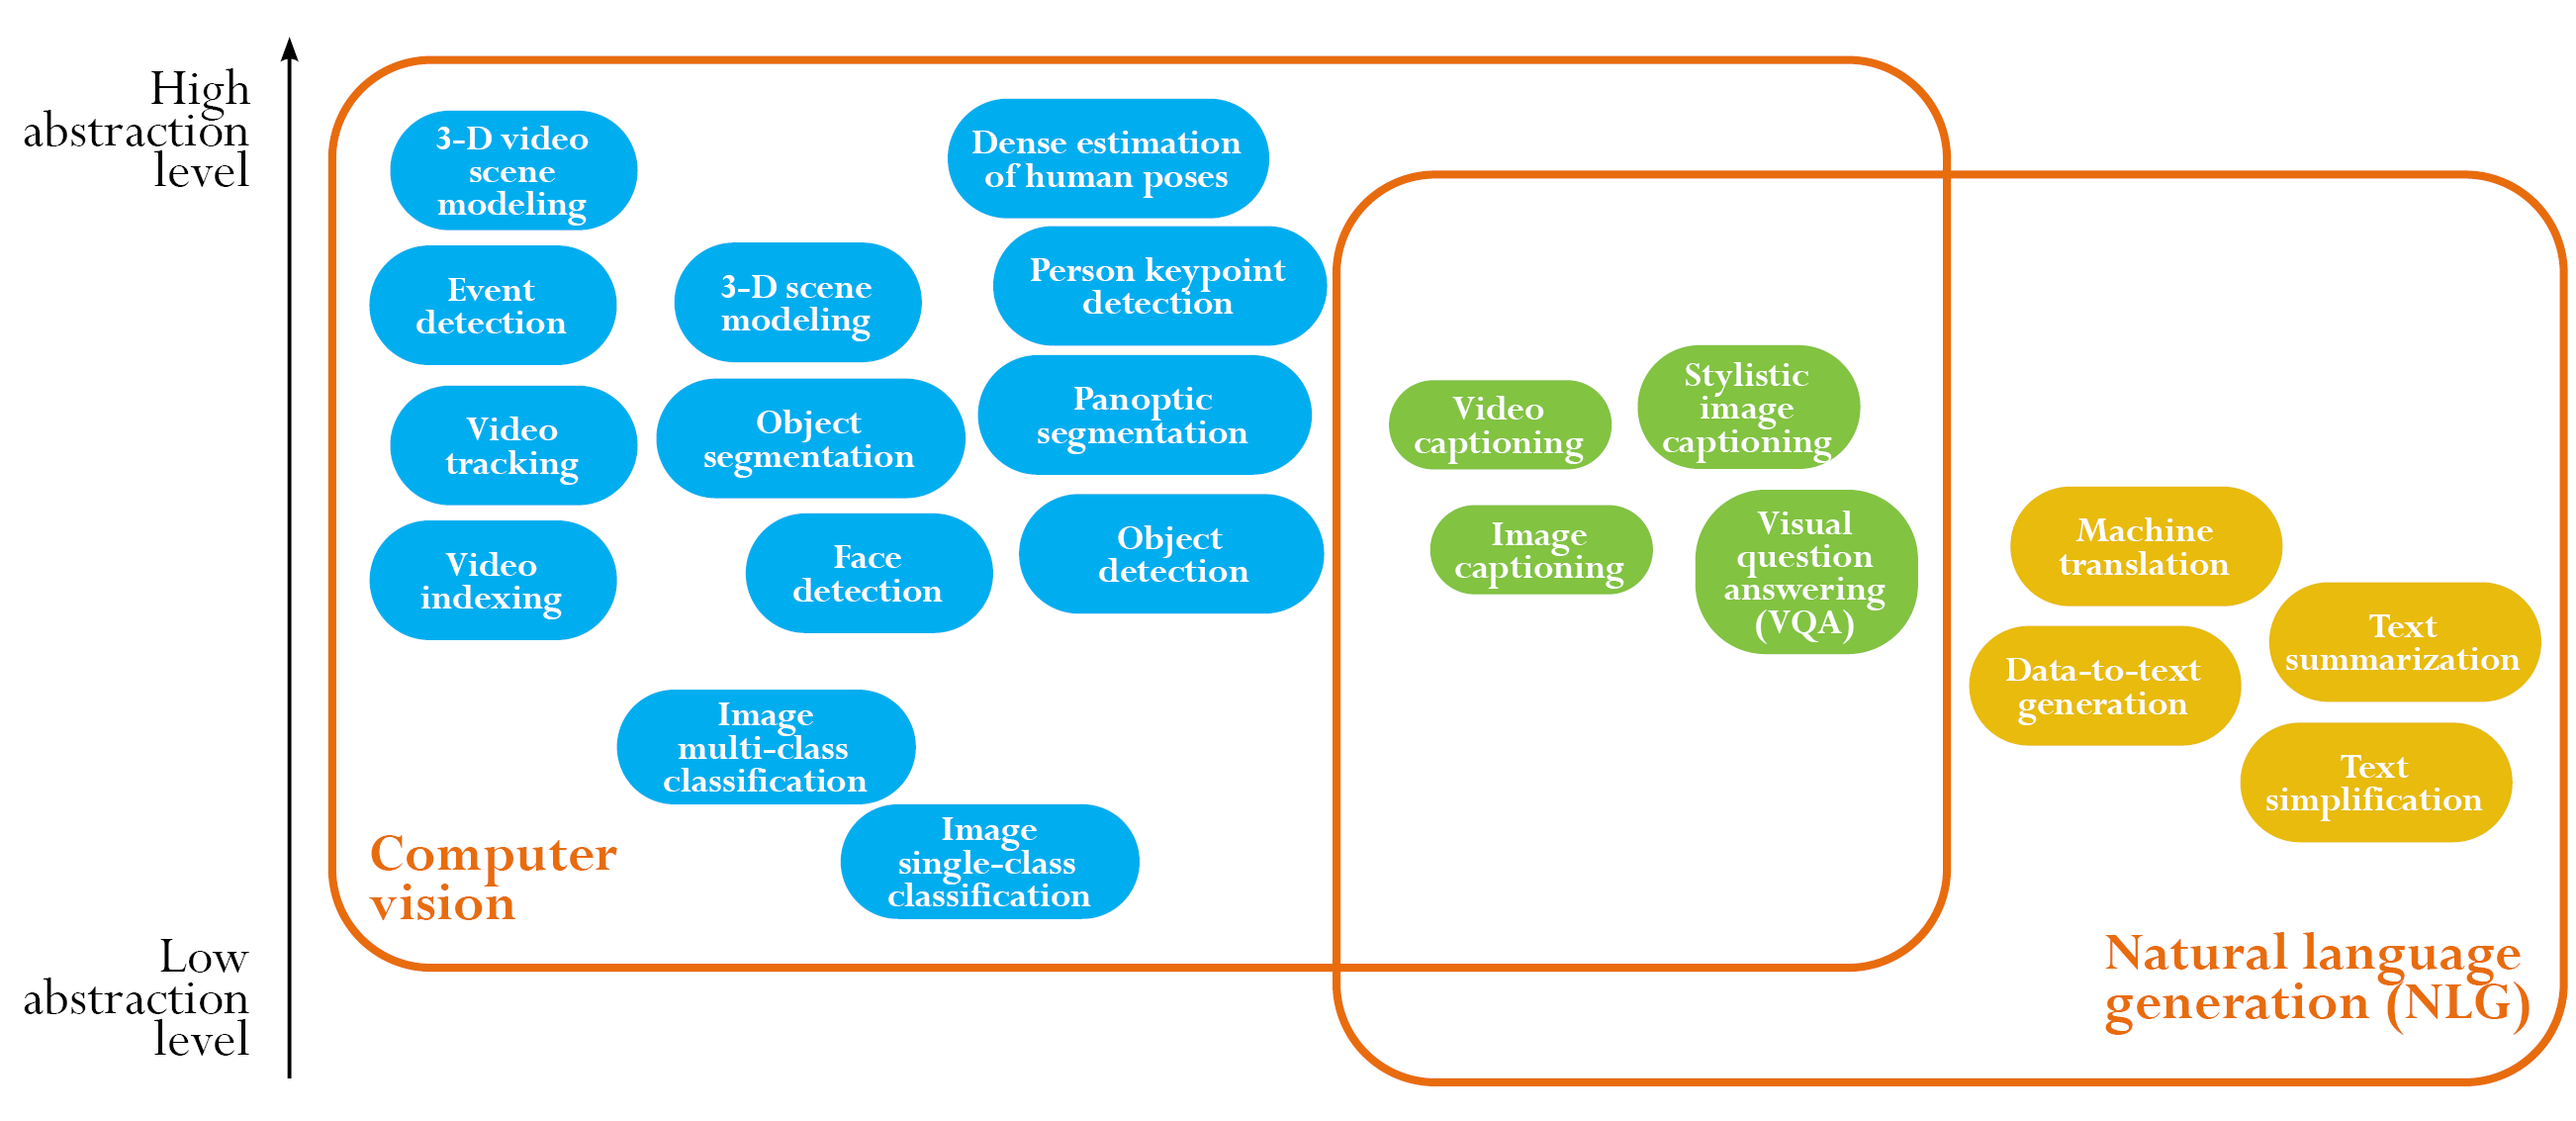
\includegraphics[width=1.0\textwidth]{./images-indesign/Task_map.png}
\caption{Image captioning and selected other machine learning tasks in the fields of computer vision and natural language generation. Abstraction level is a rough characterization.}
\label{fig:Task_map} 
\end{figure}

Besides image captioning, another practical example of a use case for scene understanding is that of a household robot (example follows Zhou et al.~\cite{zhou2017scene}): A household robot equipped with a trained convolutional network can recognize that the visual scene is a living room. However, to be able to usefully interact with the environment, for example to pick up a dirty coffee cup from the top of a table and deliver it to the kitchen sink, the robot has to be able to recognize both things like \textit{coffee cup} and \textit{table} and stuff categories like \textit{floor} and \textit{wall} within the scene to be able to navigate in the scene and pick up a coffee cup. This task requires some level of semantic understanding of the scene.

\section{Image Captioning Datasets}
\label{section:imagecaptioningdatasets}
In machine learning, datasets are often a central driving force in advancing state-of-the-art research. This is especially true for supervised learning, where a model learns to perform a task by using labeled samples in a dataset. In this section I will give an overview of selected datasets that are relevant to image captioning.

\textbf{What is Required of an Image Captioning Dataset.} Well-known datasets created for single-label or multi-label image classification tasks are not adequate for scene understanding tasks, including image captioning, for several reasons. One reason is that most image collections used for image classification tasks have images, that present objects as \textit{iconic views}~\cite{Coco}. Bicycles are depicted as seen from the side, centered in the image, unobstructed, with two tyres with spokes visible. An example of an iconic view of a bicycle is in figure \ref{fig:bicycle_iconic}. A more demanding goal for machine learning, and necessary especially in scene understanding tasks, is to be able to recognize objects also when depicted using non-iconic images or from non-canonical perspectives: partly covered by other objects, among a group of other objects, or in the background. A example of a bicycle image from a non-canonical perspective and only partially shown is in figure \ref{fig:bicycle_non_canonical}.

\begin{figure}
    \centering
    \begin{minipage}{0.45\textwidth}
        \centering
        \includegraphics[width=0.9\textwidth]{./images/bicycle_iconic.jpg}
        \caption{Bicycle in an iconic image. "Bicycle" by Conal Gallagher, CC BY 2.0.}
        \label{fig:bicycle_iconic} 
    \end{minipage}\hfill
    \begin{minipage}{0.45\textwidth}
        \centering
        \includegraphics[width=0.9\textwidth]{./images/bicycle_handlebar.jpg}
        \caption{Bicycle from a non-canonical perspective. "Bicycle and Bokeh" by Bowen Chin, CC BY-NC-ND 2.0.}
        \label{fig:bicycle_non_canonical}
    \end{minipage}
\end{figure}

A second reason for the inadequacy of image classification datasets is that object recognition has traditionally focused heavily on "thing" categories like \textit{car}, \textit{skateboard} and \textit{elephant}. For scene understanding, however, the "stuff" categories, categories that do not have clear boundaries or parts, like \textit{grass} or \textit{sky}, are very central~\cite{CocoStuff}. Caesar et al.~\cite{CocoStuff} list several reasons for the central role of stuff. For one, stuff categories often define the type of a scene: a beach scene is a beach scene because there is water and sand present. Stuff also often captures the three-dimensional structure of the scene and limits the possible locations of the thing categories. It is rare for trees to appear in water or cats to appear in the sky. Lastly, stuff provides context for identifying things, especially small things. Smaller objects in images generally require more contextual reasoning to recognize~\cite{Coco}. If there is something small in the sky, it is likely to be a bird or an aeroplane far away. As the basic version of the COCO dataset used for image captioning does not include stuff categories, and the used object detectors explicitly focus on foreground object instances, the context provided by stuff categories and full panoptic segmentation is still largely an unexplored territory for image captioning.  
Lastly, as scene understanding requires a much more detailed segmentation, labeling and annotation of an image, the sheer amount of metadata about an image is much larger in a scene understanding dataset than in an image classification dataset. Where for image multi-labeling, the metadata could only include a list of category labels ("tree", "car", "human"), for scene understanding the metadata would include pixel-level masks or bounding boxes for different object instances, attributes about each object and scene captions written by humans. An example of the object instance masks and scene captions is shown in figure \ref{fig:cocostuff-example-segmentation}.

Even if image classification datasets are not adequate for object detection, they can be used as part of the training process, especially to train the backbone network. For this reason, both simpler but larger image classification datasets and smaller but richer scene understanding datasets are important for image captioning systems. The training processes will be discussed in chapters \ref{chapter:objectdetector} to \ref{chapter:objectdetector_improvements}.

\textbf{Overview of Datasets Relevant to Image Captioning.} 
The datasets relevant to image captioning can be divided into three categories: image classification datasets, scene understanding datasets, and specialized datasets. Central image classification datasets that are presented first are ImageNet and JFT-300M. Scene understanding datasets include PASCAL VOC 2012, SUN, Flickr30k, COCO, ADE20K and Visual Genome. Finally, some relevant specialized datasets are shortly discussed: FlickrStyle10K, Personality-Captions and Localized Narratives.

\begin{table}[h] 
\centering 
\resizebox{\textwidth}{!}{%
\begin{tabular}{l| r | r | r | r | r | r} 
Dataset & Images & Categories & Captions & Cat./image & Instances/image & Year \\ 
\hline \hline 
ImageNet-21k & 14 197 122 & 21 841 & - & 1 & 1 & 2009 \\ 
ImageNet-1k (ILSVRC-2012) & 1 431 167 & 1000 & - & 1 & 1 & 
2012 \\
JFT-300M & 303 000 000 & 18 291 & - & 1.2 & 1.2 & 2017 \\
PASCAL VOC 2012 & 11 530 & 20 & - & < 2 & 2.38 & 2012 \\
SUN & 22 210 & 4479 & - & > 17 & > 17 & 2010 \\
Flickr30k & 31 783 & - & 158 915 & - & - & 2014 \\
COCO-2014 & 164 062 & 80 & 616 435 & 3.5  & 7.7 & 2014 \\
COCO & 328 124 & 80 & 616 435 & 3.5 & 7.7 & 2015 \\
COCO-Stuff & 164 062 & 172 & 616 435 & > 3.5 & > 7.7 & 2016 \\
ADE20K & 25 210 & 2693 & - & 10.5 & 19.5 & 2017 \\ 
Visual Genome & 108 077 & 33 877 & 5 406 939 & < 35 & 35 & 2017 \\
FlickrStyle10k & 7000 & - & 14 000 & - & - & 2017 \\
Personality-Captions & 201 858 & - & 241 858 & - & - & 2019 \\
Localized Narratives & 848 749 & - & 873 107 & - & - & 2020 \\

\hline
\end{tabular}}
\caption{ Comparison of datasets relevant to image captioning. The statistics marked by - are not reported or not applicable. The COCO-2014 is the dataset version used for the Microsoft COCO Image Captioning Challenge, whose scores are reported for the image captioning systems in this thesis. Data sources: ~\cite{Coco, CocoStuff, zhou2017scene, PersonalityCaptions, Flickr30kentities, VisualGenome, JFT, VisionTransformers, ImageNet21k_Pretraining} and \url{http://image-net.org/about-stats}}
\label{table:results}
\end{table}

\textbf{ImageNet}~\cite{imagenet_cvpr09, Imagenet}\footnote{See \url{https://www.image-net.org/}} is the largest of the public datasets with over 14 million images and about 22 000 object categories, more precisely stated \textit{synonym sets} (\textit{synsets}). ImageNet is organized according to the WordNet hierarchy of concepts. Each image is labeled with a single label. Due to the large size of the dataset, single-label tagging and a semantic hierarchy of concepts, the labels include inconsistencies: a very similar image of a cow is labeled "cow" in some instance and "animal" in another instance~\cite{ImageNet21k_Pretraining}. The version of ImageNet that is most commonly used in computer vision was constructed for the ImageNet Large Scale Visual Recognition Challenge (ILSVRC)~\cite{Imagenet}. An important feature of this version is that it only uses 1000 categories, and these categories were selected so that there is no overlap between the associated synsets; in practice this means that there are no parent-daughter concepts included (no "animal", only "cow), and all categories are mutually exclusive. The ILSVRC-2012 version (version of the dataset for the challenge of year 2012) is referred to as ImageNet-1k, whereas the full dataset is referred to as ImageNet-21k. ImageNet is primarily an image classification dataset, but it is very important to object detection and image captioning because it is very commonly used for training the backbones of object detectors. 

Even larger than the ImageNet, the \textbf{JFT-300M}~\cite{JFT} dataset contains 303M images with a total of 375M automatically generated labels. On average each image has 1.26 labels. There are 18 291 categories, including for example 1165 types of animals and 5720 types of vehicles. The categories form a rich hierarchy, with maximum hierarchy depth of 12 and maximum number of children per parent node being 2876. Approximately 20 \% of the labels in the dataset are noisy. The category distribution is strongly long-tailed: there are more than 2M \textit{flowers} but only 131 images of \textit{train conductors}, and 2000 categories have less than 20 images. The JFT-300M dataset is owned by Google and is not publicly available, so it has not and cannot be used as a standard dataset in scientific research. The research using the dataset cannot be reproduced, but the research community has accepted papers by Google researchers based on the dataset to be published in peer-evaluated publications.

A second category of datasets are \textit{semantic segmentation datasets}. Early well-known semantic segmentation datasets were PASCAL VOC 2012~\cite{pascal-voc-2012} and SUN. Especially SUN included significant contextual information~\cite{Coco}: it had over 17 object and stuff instances per image, making the images much more complicated and contextual than the one-object-per-image oriented ImageNet. These early datasets served primarily object detection tasks, but did not yet include descriptive captions. The \textbf{Flickr30k} dataset, published in 2014, was one of the first larger datasets that focused on providing semantic natural language descriptions, captions, for images. Using images harvested from Flickr and crowd-sourcing, this dataset provided 31 783 images with five captions each. Flick30k did not become as central as COCO in scene understanding research communities. A likely reason is that COCO had a larger number of images and provided richer metadata supporting a wider number of scene understanding tasks.

The most important semantic segmentation and image captioning dataset \textbf{COCO} was originally published during 2014 and 2015 with the name "The Microsoft Common Objects in COntext (MSCOCO) dataset"~\cite{Coco}. It has later evolved to a multi-stakeholder project and changed its name to a simpler "COCO dataset". The year 2014 part of the COCO dataset (COCO-2014) contains 123 287 training/validation images and additionally 40 775 test images, for which captions are not public. This is the dataset used in the Microsoft COCO Image Captioning Challenge, whose scores are reported for the image captioning systems in this thesis. The training/validation images of COCO-2014 are officially split as 82 783 training images and 40 504 validation images, but in practice the image captioning community uses the \textit{Karpathy split}\footnote{The Karpathy split is named after Andrej Karpathy due to Andrej Karpathy's and Li Fei-Fei's paper where it was initially introduced, see the reference.}~\cite{Karpathy}, where 113 287 images are designated as training images, 5000 as validation and 5000 as offline testing images. The second part of COCO was published in 2015, doubling the size of COCO to a total of 328 124 images. The second part of the dataset included similar images and object detection metadata as the 2014 part, but no captioning metadata. The COCO dataset has labels for 80 categories of \textit{things}, objects for which there are individual instances (person, chair, bicycle). The original COCO dataset did not include "stuff" categories, materials and objects without clear boundaries (sky, street, sand). However, in 2017, a separate Coco-Stuff project~\cite{CocoStuff} added 91 stuff categories and the category \textit{unlabeled} to the same set of images. The COCO dataset specifically aims to have non-iconic images containing objects in their natural context. One way to estimate the amount of contextual information present in an image is by calculating the average number of object categories and instances per image. The original COCO has an average of 3.5 categories and 7.7 instances per image, whereas the ImageNet has only one category per image, and PASCAL VOC has, on average, less than 2 categories and 3 instances per image. Under 10 \% of the COCO images have only one category. 

COCO only uses a predefined, closed set of entry-level categories, category labels commonly used by humans when describing objects~\cite{Coco}. Examples of entry-level categories are  \textit{dog}, \textit{chair} and \textit{person}. COCO does not use object-part categories like \textit{face}, \textit{foot} and \textit{fuselage}. The criteria for the object category selection included usefulness for practical machine learning tasks, category diversity, balance between supercategories (such as animals, vehicles and furniture), compatibility with other datasets, and availability of a large enough number of image instances containing the category. An example COCO image with the enriched COCO-Stuff segmentation is presented in figure \ref{fig:cocostuff-example-segmentation}. The full label hierarchy for COCO (including COCO-Stuff labels) in shown in figure \ref{fig:coco-labels}.

\begin{figure}[h] 
\centering
\includegraphics[width=1.0\textwidth]{./images/cocostuff-example-segmentation.png}
\caption{Example COCO image (left) with original COCO thing segmentation (center) and COCO-Stuff-augmented segmentation (right). Scene captions written by humans below the images. Image source: Caesar et al.~\cite{CocoStuff}.}
\label{fig:cocostuff-example-segmentation} 
\end{figure}

\begin{figure}[h] 
\centering
\includegraphics[width=0.9\textwidth]{./images/cocostuff-labelhierarchy.png}
\caption{Label hierarchy of the COCO thing and stuff labels. Image source: The COCO-Stuff dataset, \url{https://github.com/nightrome/cocostuff}.}
\label{fig:coco-labels} 
\end{figure}

Due to the careful label design, only 6 \% of pixels belong to the category \textit{unlabeled} in the COCO dataset augmented with stuff labels~\cite{CocoStuff}. 69,1 \% of the pixels in the COCO training and validation dataset belong to stuff and 30,9 \% to things. When considering the human-written scene captions, the stuff categories make up 38,2 \% of the nouns. This means that the stuff categories are often seen as central to describing what a scene is about and to scene understanding. The spacial context of a category can be calculated by using distance between the target category component edge and surrounding category components and the relative angle to the centre of mass of the target category component~\cite{CocoStuff}. This analysis on the COCO-Stuff dataset leads to observations like the following: trains are typically above railroads (thing-stuff); TVs are typically in front of persons (thing-thing); tiled walls are above tiled floors (stuff-stuff); and roads often have persons on both sides (stuff-thing). The support relations (such as \textit{on top of}) are semantically important, whereas side-by-side relationships are less so. Some concepts have high probabilities of occurring right next to another concept: a backpack is often right next to a person (on their back), and snowboards are almost always in the middle of snow and attached to persons.

The \textbf{ADE20K} dataset~\cite{zhou2017scene} contains 20 210 training, 2000 validation and 3000 testing images. It annotates images with a large and an unrestricted open vocabulary. The annotations include object segments with names, object parts, and attributes. ADE20K uses dense annotation, meaning every pixel has a semantic label. The usage of an open vocabulary is both a strength and a weakness of the dataset. In general, with an open vocabulary, labeling is more difficult for human annotators, and naming is more inconsistent between different annotators. The creators of the ADE20K dataset have solved the inconsistency issue by having a single expert annotator annotate the whole dataset. The used part hierarchy has a depth of 3\footnote{Full object-part hierarchy is available at \url{https://groups.csail.mit.edu/vision/datasets/ADE20K/}.}. For example, a \textit{knob} is a part of a \textit{door}, which can be part of a \textit{cabinet}. The other major issue with an open vocabulary is that there are rare object categories that appear only a few times in the whole dataset. The rare categories may be important for semantic understanding of the scene, but in practice there are too few instances for them to be useful for most machine learning algorithms. The images in ADE20K have not been manually curated to contain a similar number of instances for all caterories. As a result, the category distribution follows Zipf's law, with certain categories appearing much more frequently than others. There is an average of 10.5 object categories and 19.5 instances in an image. Any image contains at least 5 objects, and, at the largest, the number of object instances in an image is 273 (419 with part instances counted as well).

The \textbf{Visual Genome}~\cite{VisualGenome} dataset\footnote{See \url{https://visualgenome.org/}} aims to support a very detailed understanding of an image. It provides a detailed dense annotation of objects, attributes, and relationships within each image. It provides natural language descriptions for several regions of an image instead of just one description (caption) for the whole image. The dataset consists of a subset of COCO, and contains 108k images, where each image has an average of 35 objects, 26 attributes and 21 pairwise relationships between objects. On average, the region descriptions are 5 words long. A example image with all 50 region descriptions is shown in figure \ref{fig:VisualGenome_example}. The related bounding box for only 6 regions is shown in the image for clarity, but similar bounding boxes exist for all regions. Regions with only one object usually have descriptions focusing on the attributes of a single object. Regions with
two or more objects generally have descriptions about the attributes of several objects and their pairwise relationships. Each object, attribute and relationship is grounded in the image with a bounding box (these detailed bounding boxes are not shown in the sample image in figure \ref{fig:VisualGenome_example}).

\begin{figure}[h] 
\centering
\includegraphics[width=0.7\textwidth]{./images/VisualGenome_example.png}
\caption{A sample Visual Genome image with all 50 region descriptions. The related bounding box for only 6 regions is shown in the image for clarity, but similar bounding boxes exist for all 50 regions. Image source: Krishna et al.~\cite{VisualGenome}.}
\label{fig:VisualGenome_example} 
\end{figure}


Visual Genome is important for image captioning, because it was used by Anderson et al.~\cite{BottomUp} for creating rich feature vectors used by most leading image captioners. Visual Genome makes it possible to ground visual concepts -- object categories, their attributes and relations -- to image regions more firmly than just using images and image-level captions. For this dense grounding approach, looking at complimentary datasets to Visual Genome, a prominent options would be the Flickr30k Entities~\cite{Flickr30kentities}, which extends the Flickr30k with grounding the entities mentioned in captions to image regions.

The third category of datasets relevant to image captioning are specialized datasets. These datasets define metadata of an image in a more detailed way than standard scene understanding datasets such as COCO. Two datasets, FlickrStyle10k and Personality-Captions, extend the metadata with variations of language style. Localized narratives offers more explicit grounding of captions in the image.

The \textbf{FlickrStyle10k} dataset~\cite{StyleNet} takes a part of the Flickr30k dataset and augments them with additional captions with different language styles like humorous or romantic. Whereas standard captioning datasets like COCO and Flickr30k provide captions that are factual in style, FlickrStyle10k aims to teach models that can output language in specific styles, which would expand the usage contexts of models. The dataset contains 7000 images. A sample image with captions in different styles is shown in figure \ref{fig:stylenet_captions}.

\begin{figure}[h] 
\centering
\includegraphics[width=0.6\textwidth]{./images/StyleNet_captions.png}
\caption{Captions with different styles based on the FlickrStyle10k dataset. Captions created by StyleNet. Image source: Gan et al.~\cite{StyleNet}}
\label{fig:stylenet_captions} 
\end{figure}

In the \textbf{Personality-Captions}~\cite{PersonalityCaptions} dataset, the image captions are engaging and conversational in style, with each caption conditioned on one of 215 separate personality traits (for example anxious, dramatic, money-minded and humble)\footnote{Pretrained models and caption examples available at \url{https://parl.ai/projects/personality_captions/}.} The dataset consists of 241 858 captions that relate to ~200 000 images. This dataset is an interesting expansion of both the dataset metadata provided and the directly related task of generating captions with different attitudes or traits. A sample image with captions in different styles is shown in figure \ref{fig:personality_captions}.

\begin{figure}[h] 
\centering
\includegraphics[width=0.8\textwidth]{./images/Personality_captions2.png}
\caption{Sample captions using TransResNet model on the Personality-Captions dataset. Image source: Shuster et al.~\cite{PersonalityCaptions}.}
\label{fig:personality_captions}
\end{figure}

The \textbf{Localized Narratives}~\cite{LocalizedNarratives}\footnote{See data at \url{https://google.github.io/localized-narratives/}} dataset is an important recent contribution, that adds new types of annotations to several datasets, including the whole COCO, Flick30k and ADE20K. A total of 849k images are annotated. The new annotations consist of a spoken caption, transcription of the spoken caption, and related mouse traces to ground the caption segments into image regions. The annotators are asked to use their own voice to describe the images and at the same time move their mouse to point at what region of the image they are describing. These two new modalities provide a dense grounding for language in the image, at the detail level of a mouse trace segment per word. The annotators are asked to transcribe their own description immediately after giving it in spoken form, ensuring the quality of the annotations. Localized Narratives can be used for several tasks, including image captioning. As the captions in this dataset are originally provided in spoken language, they are longer than previous captions: where COCO captions have an average of 10,5 words, the Localized Narratives captions have an average of 36,5 words. This new dataset could be used to train models to write longer captions than those originally in the COCO dataset. The dense grounding of language in the image provides completely new possibilities for improving image captioner performance, including using mouse traces to guide attention at training time. A comparison of different types of captions is shown in figure \ref{fig:LocalizedNarratives_comparison}.

\begin{figure}[h] 
\centering
\includegraphics[width=1.0\textwidth]{./images/LocalizedNarratives_comparison.png}
\caption{Comparison of different types of captions. In \textit{a}, a COCO caption describes the image as a whole. In \textit{b}, a Flickr30k Entities caption grounds concrete words of the caption in the image regions. In \textit{c}, Visual Genome captions separately describe several regions of the image. In \textit{d}, a Localized Narratives caption is grounded in the image with mouse trace segments. Notice that the Localized Narratives caption was originally spoken and has been transcribed into text. Image source: Pont-Tuset et al.~\cite{LocalizedNarratives}.}
\label{fig:LocalizedNarratives_comparison}
\end{figure}

\section{Automated Evaluation Metrics}
There are several standard automated metrics (BLEU, ROUGE, METEOR, CIDEr) that are routinely used to evaluate natural language generation models on several different tasks, including image captioning. They are all calculated based on a set of reference sentences, in the case of image captioning, the ground truth captions. All of these metrics rely on evaluating overlap of $n$-grams between the produced caption and ground truth captions~\cite{SPICE}. The metrics are completely based on or oriented towards precision (BLEU), recall (ROUGE), and on a balance of precision and recall (METEOR, CIDEr). There are also different variations of the metrics, and automated NLG evaluation metrics are a field of research in its own. A captioning-specific metric, SPICE~\cite{SPICE}, takes a more ambitious semantics-oriented approach and is somewhat commonly used within the captioning task research. It is, however, not as well known as the previously mentioned four metrics, likely due to the fact that it can only be used in the captioning domain, while the others can be used for many other NLG domains. SPICE is not reported by the COCO test server. 

In this thesis, I will use the CIDEr-D c40~\cite{CIDEr} score for reporting the performance of the models. The CIDEr-D c40 is the primary metric used to rank the captioning models in the online COCO evaluation server. CIDEr (Consensus-based Image Description Evaluation) uses stemmed $n$-grams and weights them using a Term Frequency Inverse Document Frequency (TF-IDF) approach, effectively giving more weight to more informative (less frequent) expressions~\cite{CIDEr}. The point of comparison is 40 ground truth captions for each image in the COCO test test (hence the c40 postfix). It should be noted, that for the COCO training and validation sets that are available to be used for training models, only 5 captions per image exist. The 40 captions per image for the not public test set were created to get an even more broad base to evaluate the models against. 

Formally, the goal of CIDEr~\cite{CIDEr} is to automatically evaluate, for image $I_i$, how well a candidate sentence $c_i$ matches the consensus of a set of image descriptions $S_i = \{s_{i1}, s_{i2}, \text{...}, s_{im}\}$. All words in both candidate and reference sentences are first stemmed: "fish", "fishing" and "fished" all get reduced to "fish". The sentences with stemmed words are then each represented as a set of one or more ordered words that are present in the sentence, $n$-grams. The $n$-grams of the candidate sentence are then compared to the reference sentences: a good candidate sentence is one that has $n$-grams, that are also present in the reference sentences and does not have $n$-grams that are not found in the reference sentences. $n$-grams that are common in many captions in the dataset are less informative, and should be given lower weight. The number of times an $n$-gram $\omega_k$, where $k$ is an index, occurs in a reference sentence $s_{ij}$ is denoted by $h_k(s_{ij})$, and the number of times it appears in a candidate sentence by $h_k(c_i)$. The TF-IDF weighting $g_k(s_{ij})$ for each n-gram $\omega_k$ is computed using the equation
\begin{equation}
g_k(s_{ij}) = \frac{h_k(s_{ij})}{\sum_{\omega_l \in \Omega} h_l(s_{ij})} \log \left( \frac{\lvert I \rvert}{\sum_{I_p \in I} \text{min}(1, \sum_q h_k(s_{pq}))} \right)
\end{equation}
%
where $l$ is a set of $n$-grams that appear in the corpus (set of words in case of $n=1$), and $I$ is the set of all images in the dataset. The first term on the right side of the equation is the term frequency. In the case of $n=1$, for example the word "cat" could occur 500 times in a set of captions containing a total of 10 000 words, and would then have $\text{TF}(\text{cat}) = 500 / 10 000 = 0.05$. The second term on the right side of the equation, IDF, measures the rarity of an $n$-gram $\omega_k$. It reduces the weight of those $n$-grams that commonly appear across many captions in the dataset. IDF is computed using the logarithm of
the number of images in the dataset $\lvert I \rvert$ divided by the number of images for which $\omega_k$ occurs in any of its reference sentences. In the $n=1$ case, words like "person" will have a low IDF, as they are found in very many images and related ground truth caption sets.

The CIDEr score for $n$-grams of length $n$ is calculated using average cosine similarity between the candidate sentence and reference sentences:
\begin{equation}
\text{CIDEr}_n(c_i, S_i) = \frac{1}{m} \sum_j \frac{\vect{g^n}(c_i) \cdot \vect{g^n}(s_{ij})}{\left\lVert \vect{g^n}(c_i) \right\rVert \left\lVert \vect{g^n}(s_{ij}) \right\rVert}
\end{equation}
%
where $\vect{g^n}(c_i)$ is a vector calculated by concatenating the TF-IDF weightings $g_k(c_i)$ of all $n$-grams of length $n$ in the candidate sentence $c_i$, $\left\lVert \vect{g^n}(c_i) \right\rVert$ is the length of that vector, and $\vect{g^n}(s_{ij})$ and $\left\lVert \vect{g^n}(s_{ij}) \right\rVert$ similarly for the set of reference captions for the image.

The final CIDEr score is calculated by summing the $n$-gram CIDEr scores for $n$-grams of length 1, 2, 3 and 4:
\begin{equation}
\text{CIDEr}(c_i, S_i) = \sum_{n=1}^4 w_n \text{CIDEr}_n(c_i, S_i)
\end{equation}
%
The scaling factor $w_n$ would make it possible to give more emphasis to either shorter or longer $n$-grams, but CIDEr uses uniform weights, and sets $w_n = 1 / N$.

CIDEr reflects well the human perception of model performance on the captioning task. CIDEr-D is a modification of the basic CIDEr that aims to eliminate gaming possibilities of the metric. It achieves this by not stemming words, introducing a penalty for differing sentence length between target and ground truth, and penalizing the repetition of specific $n$-grams beyond the number of times they occur in the reference sentence. The CIDEr-D~\cite{CIDEr} variants of the already described CIDEr equations are:
\begin{equation}
\text{CIDEr-D}_n(c_i, S_i) = \frac{10}{m} \sum_j e^{\frac{- (l(c_i)-l(s_{ij}))^2}{2\sigma^2}} * \frac{\text{min} ( \vect{g^n}(c_i), \vect{g^n}(s_{ij})) \cdot \vect{g^n}(s_{ij})}{\left\lVert \vect{g^n}(c_i) \right\rVert \left\lVert \vect{g^n}(s_{ij}) \right\rVert}
\end{equation}
\begin{equation}
\text{CIDEr-D}(c_i, S_i) = \sum_{n=1}^4 w_n \text{CIDEr-D}_n(c_i, S_i)
\end{equation}
%
where $l(c_i)$ denotes the length of a candidate sentence, $l(s_{ij})$ denotes the length of the reference sentences, $\sigma$ is a constant ($\sigma$ = 6), and scaling factor $w_n = 1 / N$ is again uniform. The constant factor of 10 is added to make CIDEr-D numerically similar to other metrics, especially the standard CIDEr. The CIDEr authors report~\cite{CIDEr} that the CIDER-D version of the metric has a rank correlation of 0.94 with the original CIDEr metric while being more robust to gaming.

The CIDEr-D variant of CIDEr is used by the COCO online server and in this thesis. For all the models, a wider set of metrics (c40 versions of BLEU-1, BLEU-2, BLEU-3, BLEU-4, METEOR, ROUGE-L, CIDEr-D), all provided by the COCO online test server, are reported in Appendix \ref{appendix:cocoresults}. 

The top COCO evaluation server CIDEr-D c40 score as of 31.3.2021 23:59:59 UTC was 1.387 by the entry MSR-MS\_Cog\_Svcs (presumably a Microsoft Cognitive Services based team), which does not currently have a related published research paper, code or other information to accompany it.

\chapter{Object Detection in Leading Image Captioning Systems}
\label{chapter:objectdetector}

\textit{Features matter.} \\
\textit{- Ross Girshick, Jeff Donahue, Trevor Darrell and Jitendra Malik} \\
\\
%
All leading image captioners use an object detection network to calculate the object detections and their feature vectors as input for the image captioning network. Interestingly, all the leading image captioners under investigation use the \textit{same} object detector, the Bottom-Up object detector by Anderson et al.~\cite{BottomUp}, which is in turn based on the Faster R-CNN~\cite{FasterRCNN}. The object detector arguably does a large part of the work of an image captioner, and therefore is in fact an essential part of the image captioning system. In this chapter, I will present the object detection network used by the image captioners. In the next chapter (\ref{chapter:captioners}), I will present the image captioner components of the systems. Later, in chapters \ref{chapter:backbone} and \ref{chapter:objectdetector_improvements}, I will investigate ways to further improve the backbone and object detector components of the image captioning system.

\textit{Object detection} is a process where all areas of an image containing objects of interest are bounded, while areas of the image that are not part of these objects are ignored~\cite{PolyYOLO}. The most straightforward way to bound the object instances is to define a bounding box around each object instance. The bounding boxes are usually defined using spatial coordinates of its top-left corner and its width and height. The downside of the bounding box approach is that for objects that are partially occluded by other objects or have very complex shapes, a notable amount of pixels within the bounding box does not actually belong to the object instance. In response to this problem, more fine-grained approaches of bounding the object instance using polygons~\cite{PolyYOLO} or a pixel-level mask~\cite{MaskRCNN} are also used. The more fine-grained approaches are closely related to the bounding box approach, and can often be computed in sequence or in parallel within the same pipeline or end-to-end-model~\cite{PolyYOLO, DETR}. All of the leading image captioning methods under investigation use feature vectors based on bounding box object detections. 

\section{Faster R-CNN}
Faster R-CNN is an evolution of the Fast R-CNN~\cite{FastRCNN} (Fast Region-based Convolutional Network), which was published by Ross Girshick in 2015. The Fast R-CNN is an object detector, which builds on the work of CNNs used for object classifications (like VGG-16) and the earlier (2014) ground-breaking work on the R-CNN~\cite{RCNN} model.

\textbf{R-CNN.} R-CNN~\cite{RCNN} introduced many of the central techniques used by Fast R-CNN, Faster R-CNN and through it, also the image captioners under investigation. It extracted a large number (about 2000) category-independent region proposals for the input image, then extracted a fixed-length feature vector for each proposal, and then classified each region as belonging to an object category~\cite{RCNN}. It also used the techniques of \textit{affine image warping} to compute a fixed-size CNN input from each region proposal, independent of the region's shape, \textit{greedy non-maximum suppression} to find unique object instances from a larger set of potential object instances, and \textit{bounding box regression} to learn correct locations for object instances. Another contribution, still valid and in use, was using supervised pretraining of the CNN on a large auxiliary dataset (ImageNet), followed by domain-specific fine-tuning on a smaller dataset (in R-CNN case Pascal VOC), a technique that later came to be known as transfer learning. An important feature of the R-CNN was that it was agnostic of the region proposal process, being compatible with several ways of producing region proposals. It did utilize the selective search technique to demonstrate the approach in practice.

\textbf{Fast R-CNN.} Fast R-CNN addressed the main problems of the R-CNN: slow and space-demanding multi-stage training and slow test-time performance~\cite{FastRCNN}. It used the VGG16 as the backbone CNN, trained the whole network in one stage and updated not only the custom object-detection layers, but also the backbone convolutional layers. It also replaced R-CNN's support vector machines in the object detector with region of interest (RoI) pooling, fully connected layers and a softmax layer. The region of interest pooling layer extracted a fixed-length feature vector for each object proposal from the shared feature map produced by the backbone CNN. In practice, RoI pooling worked by dividing a RoI window of height $h$ and width $w$ into a grid of sub-windows $H \times W$ of approximate size $h/H \times w/W$, and then max-pooling the values in each sub-window into one output cell. The max pooling was applied independently to each feature map channel. The typical size of the fixed-size feature map after RoI max pooling was $7 \times 7 \times 512$. The two fully connected layers after RoI max pooling were 4096 units wide. Architecture of Fast R-CNN is shown in figure \ref{fig:architecture_Fast_R-CNN}. Fast R-CNN used a multi-task loss function to simultaneously learn to output the correct object category and a bounding box for the object instance~\cite{FastRCNN}.

\begin{figure}[h] 
\centering
\includegraphics[width=0.9\textwidth]{./images/Fast_R-CNN_architecture.png}
\caption{Architecture of Fast R-CNN. Note that the architecture does not include how to create object proposals. Image source: Girshick~\cite{FastRCNN}.}
\label{fig:architecture_Fast_R-CNN} 
\end{figure}

\textbf{Faster R-CNN.} The Fast R-CNN was still agnostic as to how to extract the object proposals. Faster R-CNN~\cite{FasterRCNN} evolved Fast R-CNN by introducing the region proposal network (RPN), sharing convolutional layers between the RPN and object detector, and hence implementing the region proposal process and per-region feature extraction in an efficient way. A region proposal network is a fully convolutional network that predicts object bounds and objectness scores for several anchor positions. The RPN effectively works as an attention mechanism, telling the object detector where in the image to look. Faster R-CNN also introduced \textit{anchor boxes}, reference points, which were used to examine proposals at multiple scales and aspect ratios. The architecture of the region proposal network is shown in figure \ref{fig:architecture_RPN}.

\begin{figure}[h] 
\centering
\includegraphics[width=0.7\textwidth]{./images/RPN_architecture.png}
\caption{Structure of the region proposal network (RPN) in Faster R-CNN. Note especially the anchor boxes with varying sizes and ratios. Typically there would be 9 anchor boxes per position. The convolutional feature map shown is a mid- to high-level map from the backbone CNN (see e.g. figure \ref{fig:architecture_M2} for more details on the complete architecture). Image source: Ren et al.~\cite{FasterRCNN}.}
\label{fig:architecture_RPN} 
\end{figure}

In the RPN training, positive objectness classification is assigned to any anchor box with the highest intersection-over-union (IoU)\footnote{\textit{Intersection-over-union} is calculated simply by counting the pixels of the ground truth box and the predicted box that intersect (are in both boxes) and dividing it with the number of pixels in the union (are in at least one of the boxes). In practice this gives a statistic on how well the predicted box is aligned with the ground truth box.} overlap with a ground-truth box, or an anchor that has an IoU overlap higher than 0.7 with any ground truth box. This means that there can be several anchors associated with a single ground-truth box at this stage. On the other hand, a negative classification label is assigned to any non-positive anchor if its IoU is less than 0.3 for all ground-truth boxes. Anchors that are not either positive nor negative do not contribute to the training objective.

With Faster R-CNN, the typical amount of proposals per image was still 2000 at training time, but was reduced from 2000 down to 300 at test time, making the inference very fast compared to Fast R-CNN~\cite{FasterRCNN}. Due to the non-maximum suppression, there actually is a variable amount of object proposals, often much less than 300. 

In the original Faster R-CNN paper~\cite{FasterRCNN}, alternating optimization was used. Alternating optimization meant training the object detector and shared convolutional layers while keeping the RPN frozen, then switching to training the RPN and convolutional layers, while keeping object detector layers frozen, and iterating. Later the authors stated that approximate joint optimization produces similar quality results, but trains faster\footnote{See original Python implementation at \url{https://github.com/rbgirshick/py-faster-rcnn} and Ross Girshick's presentation at \url{https://www.dropbox.com/s/xtr4yd4i5e0vw8g/iccv15_tutorial_training_rbg.pdf?dl=0}}. In the approximate joint optimization, there are four loss functions: objectness classification and bounding box regression in the RPN and object classification and bounding box regression in the object detector. 

Faster R-CNN is compatible with different backbones. Already in 2015, the original backbone VGG16 was replaced with ResNet-101, and the upgraded Faster R-CNN won several leading object detection and image classification competitions~\cite{FasterRCNN}. Some sample object detections using Faster R-CNN on COCO images are shown in figure \ref{fig:sample_detections_Faster_R-CNN}.

\begin{figure}[h] 
\centering
\includegraphics[width=1.0\textwidth]{./images/FasterRCNN_sample_detections_COCO.png}
\caption{Sample object instance detections on some COCO images. The object detector is detecting the 80 categories present in the COCO dataset. The network is Faster R-CNN with VGG16 as backbone. An object category softmax score threshold of 0.6 is used for displaying a detection. Image source: Ren et al.~\cite{FasterRCNN}.}
\label{fig:sample_detections_Faster_R-CNN} 
\end{figure}

Faster R-CNN had been modified for semantic segmentation already when the article was released in 2015. The standard panoptic and semantic segmentation extension, published in 2017, is Mask R-CNN~\cite{MaskRCNN}, which extends Faster R-CNN by predicting object masks for all object instances in parallel with the bounding box recognition process. It is still used in leading object detection platforms and libraries, for example the Detectron2 platform\footnote{See \url{https://github.com/facebookresearch/detectron2}.} by Facebook AI Research.

\section{Bottom-Up and Top-Down}
In their 2018 paper, Anderson et al.~\cite{BottomUp} present a technique for image captioning, where they use a Faster R-CNN based network to determine the regions of interest of an image in a bottom-up fashion, and then use the feature vectors associated with each region in a top-down manner to determine feature weightings to use in image captioning and visual question answering (VQA). The leading image captioners being examined in this thesis still use a very similar high-level approach. More importantly, all leading image captioners\footnote{Except for X-Linear Attention Network, which originally uses ResNet-101 and the provided features, but improves by swapping the backbone to SENet-154 and recalculates the features using Bottom-Up.} directly use the object detections and feature vectors calculated by the Bottom-Up and Top-Down authors as input into their high-level image encoders and language decoders\footnote{Feature vectors are available at \url{https://github.com/peteanderson80/bottom-up-attention}. Both fixed 36 object instances per image and the adaptive 10 to 100 object instances per image are available as precalculated feature vectors for the whole COCO dataset.}. Effectively these methods are using the object detector built by Anderson et al. as a part of their image captioning system. Therefore it is important to examine in detail the object detector part of their work. The image captioner is not examined at a similar level of detail, since the state-of-the-art image captioners have later improved on that part.

The Bottom-Up and Top-Down method implements their object detector based on Faster R-CNN with ResNet-101 as the backbone. A major contribution is generating more rich feature vectors thanks to training the object detector using object and attribute annotations from the Visual Genome dataset~\cite{VisualGenome}. The attributes are learned through adding a new loss function, object attribute loss, to the four existing loss functions of the Faster R-CNN (bounding box regression and objectness in RPN and bounding box regression and object classification in object detector). The five loss functions and the architecture of the Bottom-Up object detector, including the ResNet-101 backbone, is presented in the architecture diagrams of the leading image captioners in chapter \ref{chapter:captioners}, for example in figure \ref{fig:architecture_AoA}. 

The Visual Genome (VG) data set  is used with a train-eval-test split of 98k/5k/5k, ensuring that the images that are contained in both COCO and Visual Genome (51k) are all in matching splits of the two datasets~\cite{BottomUp}. As VG object and attribute annotations are free-form text, heavy preprocessing of the annotations is applied: abstract classes are removed, and a structured set of 1600 object classes and 400 attribute classes is extracted. An important decision is not to merge or remove overlapping classes (like \textit{person}, \textit{man}, \textit{guy}), classes with singular and plural formulations (like \textit{tree} and \textit{trees}), or stuff classes (like \textit{sky} or \textit{grass}). This richness of classes at training time contributes to creation of rich feature vectors, the true end goal of the object detector as a part of an image captioning system.

Non-maximum suppression is performed at the late object detection layers for each object class using an IoU threshold of 0.3 and for each bounding box using an IoU threshold of 0.7~\cite{BottomUpSupplement}. Then all regions where any class detection probability exceeds a confidence threshold of 0.2 are selected. For each selected region $i$, the feature vector $v_i$ is calculated as a mean-pooled, 2048-dimensional vector based on the backbone CNN features of that area~\cite{BottomUp}.

In the paper~\cite{BottomUp}, the authors initially allow the number of regions per image to vary with the complexity of the image, up to a maximum of 100. They, however, note, that selecting only the top 36 regions per image works nearly as well in the downstream image captioning and visual Q\&A tasks. 

There are several reasons, why the Bottom-Up and Top-Down captioning approach -- which is inherited by the current leading image captioners -- is so successful. One reason is that it can attend to both fine details and large image regions, thanks to the multi-scale, multi-ratio region proposals of the Faster R-CNN. A second reason is that the feature vectors are rich, containing a representation of all the visual attributes and concepts associated with the object. This enables processing all the information related to an object at once. The authors also note some similarities to the visual processing mechanisms in the human brain~\cite{BottomUp}. 

\chapter{Overview of Leading Image Captioners}
\label{chapter:captioners}

In this chapter, I will investigate the architectures and contributions of the five image captioning systems under investigation: Attention on Attention~\cite{AoA}, the Meshed-Memory Transformer~\cite{M2}, the X-Linear Attention Network~\cite{XLinearAN}, the Show, Edit and Tell~\cite{ShowEdit} method, and Prophet Attention~\cite{Prophet}. The chosen image captioning systems and their basic statistics are shown in table \ref{table:captioning_systems}. These systems were chosen, because they were the top methods found by following cross-references between captioning publications and searching through Google Scholar, with the exception of Show, Edit and Tell. Show, Edit and Tell was chosen due to a complimentary approach to captioning and taking into account that the COCO test server score was achieved using a single model, not an ensemble like in the other cases. 

\begin{table}[h] 
\centering 
\resizebox{\textwidth}{!}{%
\begin{tabular}{l| r | r | r | r | r | r} 
Captioning system & CIDEr-D c40 score & COCO online server rank 31.3.2021 & Year \\ 
\hline \hline 
Attention on Attention & 1.296 & \#34 & 2019 \\
Meshed-Memory Transformer & 1.321 & \#21 & 2019 \\
X-Linear Attention Network & 1.335 & \#13 & 2020 \\
Show, Edit and Tell & 1.257 & \#64 & 2020 \\
Prophet Attention & 1.337 & \#11 & 2020 \\

\hline
\end{tabular}}
\caption{Image captioning systems chosen for investigation.}
\label{table:captioning_systems}
\end{table}

As already stated, all leading image captioning systems under investigation rely on the Bottom-Up object detector presented in the previous chapter. In this chapter, I will present architecture diagrams of the systems as a whole, including the backbone CNN and object detector layers. Even if all currently leading image captioners are effectively two-part systems, where the image captioning layers use only the feature vectors output by the object detector, it is important to keep in mind, that this kind of a split system with a well-defined bottleneck interface between the two parts is not the only possible architecture. Developing this top-level architecture will be discussed in chapter \ref{chapter:improving_system}. 

As the systems are effectively two-part systems, the training of the systems is also done in more than one stage. All described image captioning systems share a similar three-stage training process, which is described in detail in the section on the Meshed-Memory Transformer (section \ref{section:Meshed-Memory_Transformer}). The first stage is related to training the backbone, second to the object detector and the third to the image captioning components. There is some variation in the training within this third stage, and this variation in described in conjunction with each captioner.

The captioning systems under investigation have all (except Show, Edit and Tell) been \#1 or very close to the top on the COCO Image Captioning Challenge leaderboard when they have been published. At the time of this investigation (31.3.2021), there are already some newer entries to the COCO challenge, that have achieved higher scores than the five entries under investigation. New high-scoring entries are made almost daily, so the exact rankings change constantly. As captioning is an active research area with commercial applications, it is likely that some of the top entries have been made by professional commercial teams and may never be published. Based on the names of the entries, some of the top entries are likely by teams at  Microsoft (MSR-MS\_Cog\_Svcs) and the National Laboratory of Pattern Recognition at the Chinese Academy of Science (IVA-CASIA). As the cycle of developing new methods in the academia is such, that test server runs are usually done 3-6 months before publishing a related research paper, it is also possible that some of the top COCO test server entries per 31.3.2021 will be published during 2021. The CIDEr-D c40 scores of the top 100 entries are between 1.387 and 1.210, with the top 32 entries being above 1.3, so it is likely that there are no major unpublished breakthroughs -- this kind of breakthrough should result in notably higher scores. The chosen methods do therefore represent the current state-of-the-art of captioning methods.

\pagebreak
\begin{figure}[H] 
\centering
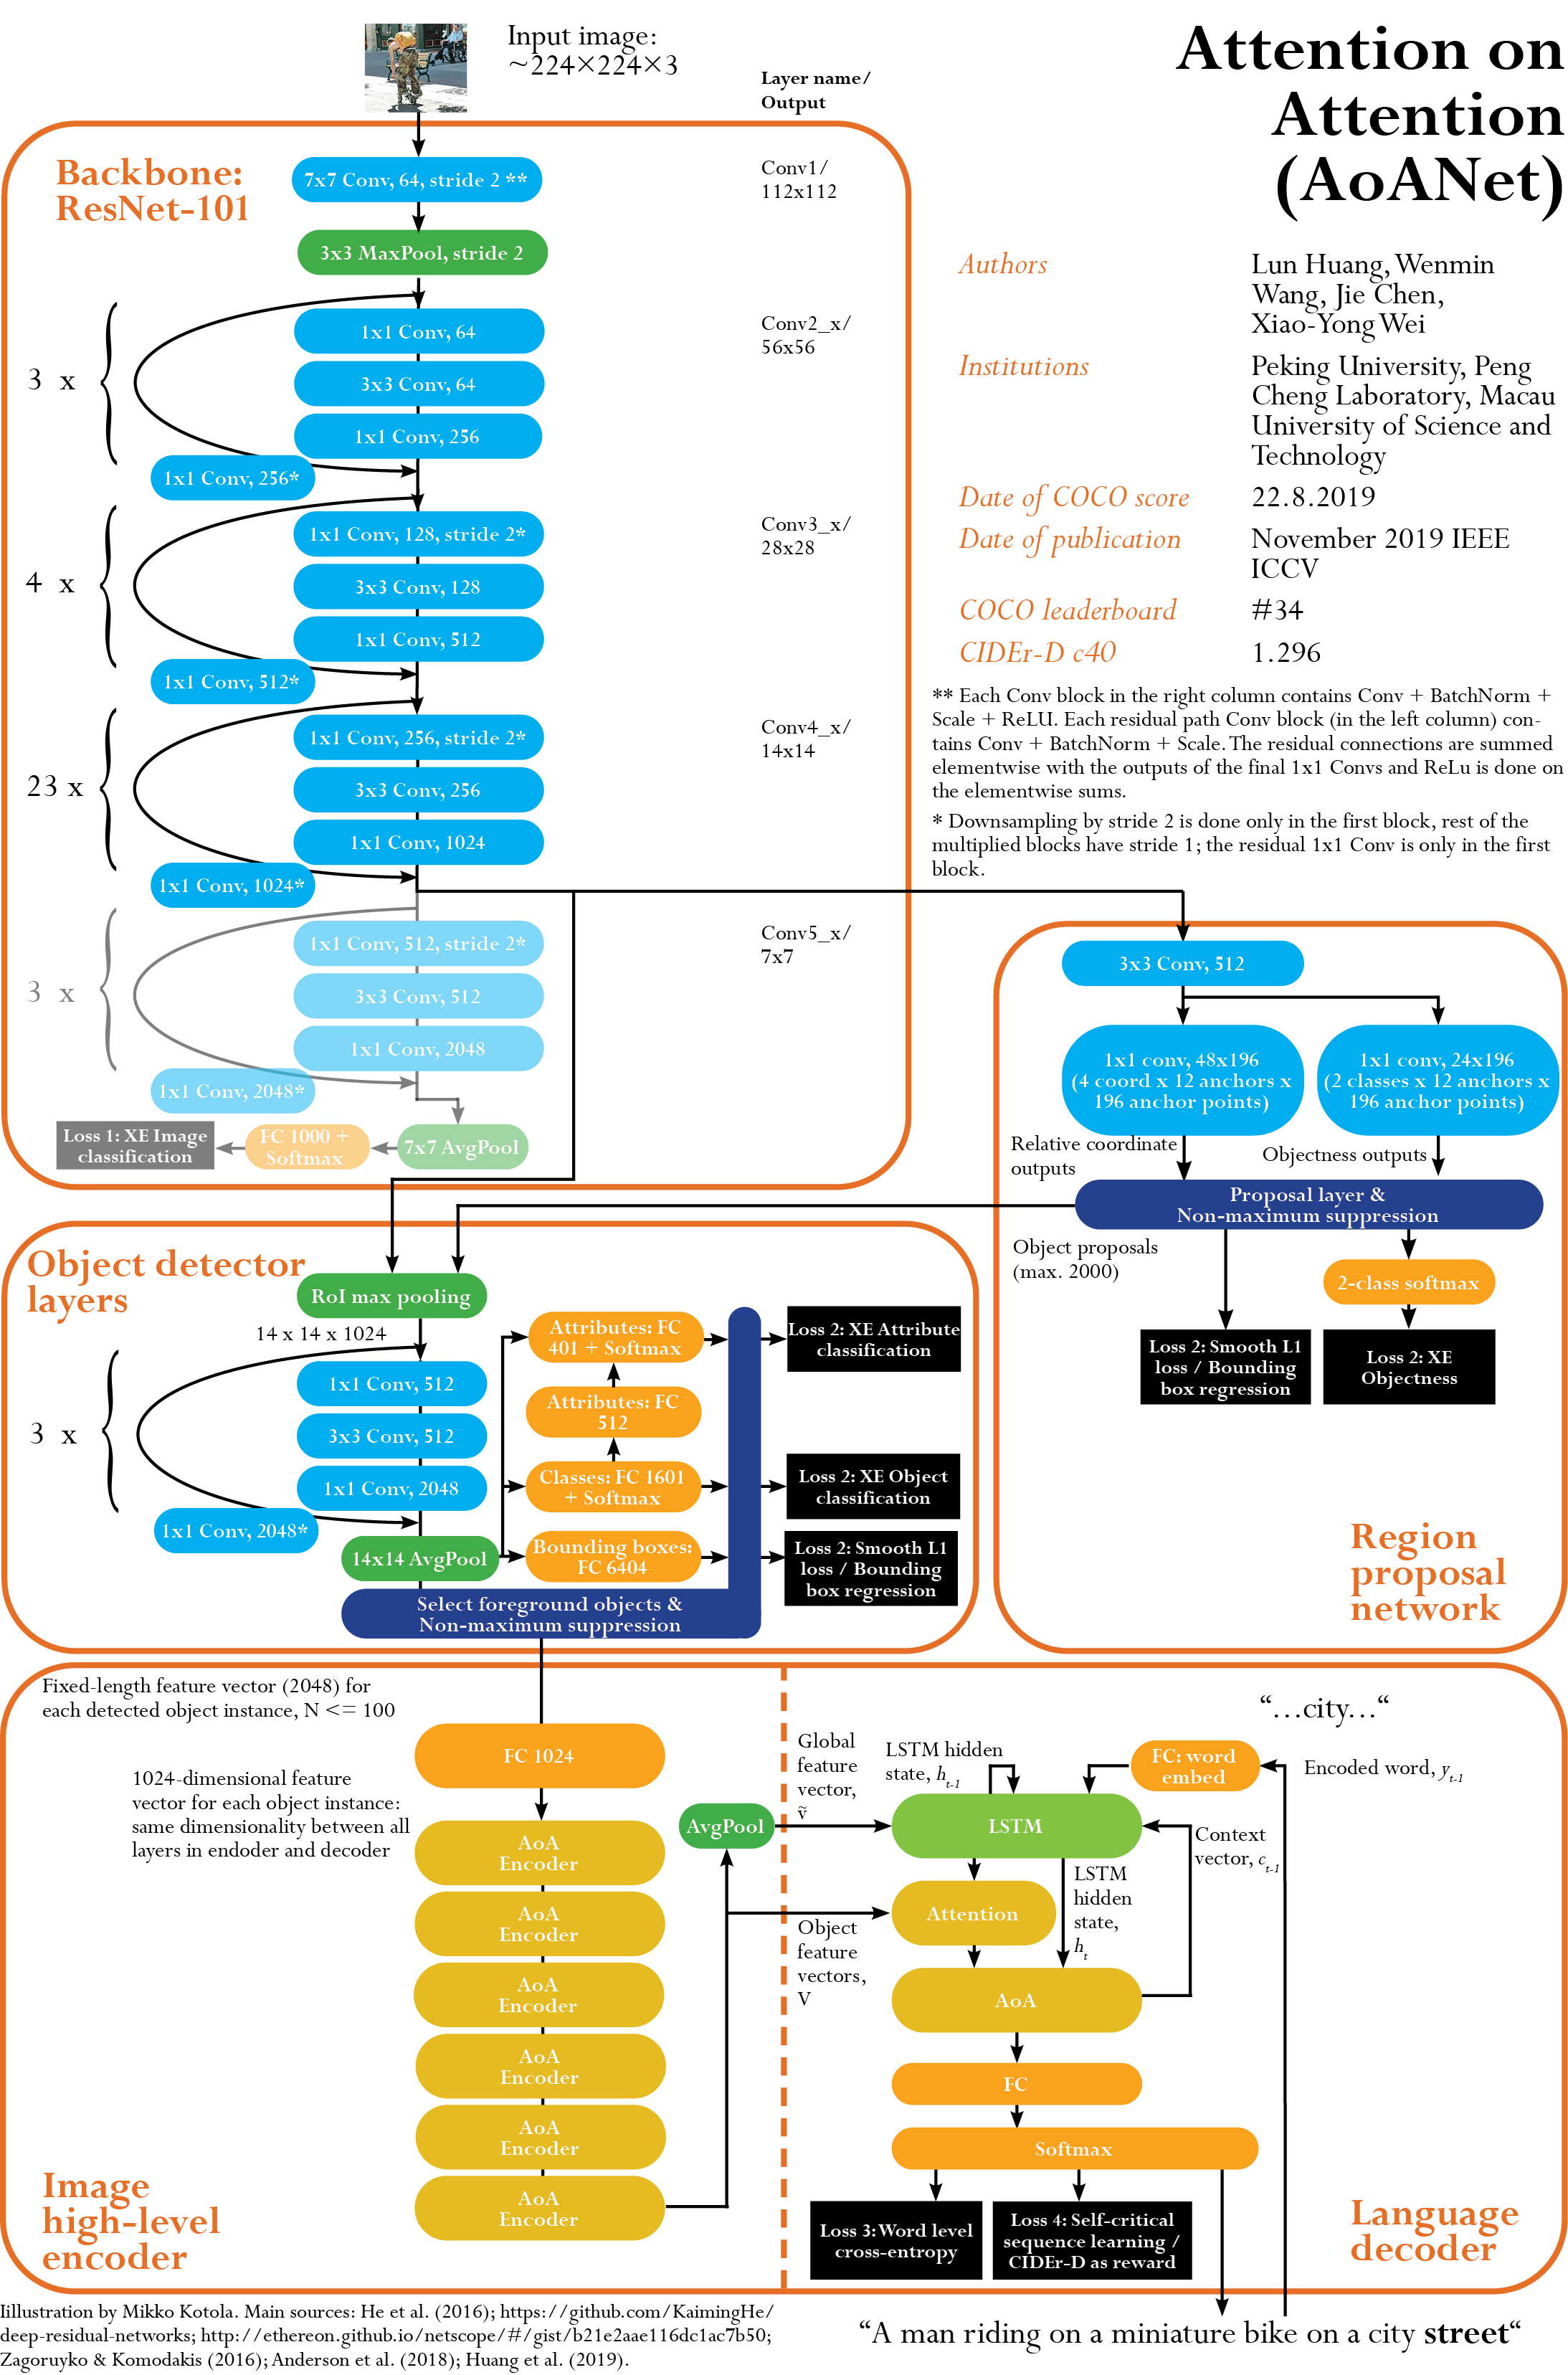
\includegraphics[width=1.0\textwidth]{./images-indesign/Architecture_AoA.png}
\caption{Architecture of the complete AoANet system.}
\label{fig:architecture_AoA} 
\end{figure}

\section{Attention on Attention}
Attention-based encoder-decoder captioners generally rely on the attention mechanism to guide the decoding process by generating a weighted average over the extracted feature vectors for each time step. Huang et al.~\cite{AoA} note that in earlier attention-based captioning models, the attended image-based vector at some time-step of the decoding process and the language-context based attention query are not always equally related. In some time-steps the decoder has to output filler words or abstract words not necessarily grounded in any image regions, but more purely on the state of the language decoder. This can lead to the decoder giving a misled output. The attention on attention based model \textit{AoANet} solves this problem by introducing a second layer of attention, enabling the model to adjust its degree of attending to the image feature encodings and the language context. The main idea of the model is presented in figure \ref{fig:AoA_idea}. I will first discuss the general AoA module, which is the way of extending the plain transformer module to include second order attention. I will then describe how the AoA module is used to build an image captioner, AoANet. The architecture of the complete AoANet-based captioning system is shown in figure \ref{fig:architecture_AoA}.

\begin{figure}
    \centering
    \begin{minipage}[t]{0.45\textwidth}
        \centering
        \includegraphics[width=\textwidth]{./images/AoA_idea.png}
        \caption{Attention on Attention model calculates an information vector and an attention gate using the attention result and the attention query. Then a second level attention mechanism is added by applying the gate to the information, resulting in the attended information vector. Image source: Huang et al.~\cite{AoA}.}
        \label{fig:AoA_idea} 
    \end{minipage}\hfill
    \begin{minipage}[t]{0.45\textwidth}
        \centering
        \includegraphics[width=\textwidth]{./images/AoA_comparison.png}
        \caption{Comparison of the structure of plain attention and Attention on Attention blocks. Image source: Huang et al.~\cite{AoA}.}
        \label{fig:AoA_comparison}
    \end{minipage}
\end{figure}

\textbf{Attention on Attention module.} The plain attention module $f_{\text{att}}(\matr{Q}, \matr{K}, \matr{V} )$ operates on queries $\matr{Q}$, keys $\matr{K}$ and values $\matr{V}$ and generates weighted average vectors $\hat{\vect{v}} = f_{\text{att}}(\matr{Q}, \matr{K}, \matr{V})$~\cite{AoA}. First, similarity scores between queries and keys are calculated, usually by calculating a dot product between the vectors:
\begin{equation}
\vect{a}_{\text{i,j}} = f_{\text{sim}}(\vect{q}_i, \vect{k}_j)
\end{equation}
%
Then a softmax function is applied to the similarity scores to get attention weights:
\begin{equation}
\vect{\alpha}_{\text{i,j}} = \frac{e^{\vect{a}_{\text{i,j}}}}{\sum_{j}e^{\vect{a}_{\text{i,j}}}}
\end{equation}
%
And finally the attention weights are multiplied with the value vectors to get attention results:
\begin{equation}
\hat{\vect{v}}_{i} = \sum_{j}\vect{\alpha}_{\text{i,j}} \vect{v}_{j}
\end{equation}
%
These three equations correspond to the plain attention module visualized on left side of figure \ref{fig:AoA_comparison}. Here, $\vect{q}_i \in \matr{Q}$ is the $i$th query, $\vect{k}_j \in \matr{K}$ and $\vect{v}_j \in \matr{V}$ are the $j$th key/value pair, $f_{\text{sim}}$ is a function that gives the similarity score of each $\vect{k}_j$ and $\vect{q}_i$, and $\hat{\vect{v}}_i$ is the attended vector for the query $\vect{q}_i$.

As visualized on the right side of figure \ref{fig:AoA_comparison}, AoA takes the result of the plain attention module $\hat{\vect{v}}$ and concatenates the original query vector with it. It then calculates two linear transformations~\cite{AoA}, the information vector $\vect{i}$ and the attention gate $\vect{g}$:
\begin{equation}
\vect{i} = \matr{W}_{q}^{i} \vect{q} + \matr{W}_{v}^{i}\hat{\vect{v}} + \vect{b}^i
\end{equation}
\begin{equation}
\vect{g} = \sigma(\matr{W}_{q}^{g} \vect{q} + \matr{W}_{v}^{g}\hat{\vect{v}} + \vect{b}^g)
\end{equation}
%
where $\sigma$ is the sigmoid activation function and $\matr{W}_{q}^{i} \text{, } \matr{W}_{v}^{i} \text{, } \matr{W}_{q}^{g} \text{, } \matr{W}_{v}^{g} \in \mathbb{R}^{D \times D}$ are embedding matrices, $\vect{b}^i \text{, } \vect{b}^g \in \mathbb{R}^D$ are bias vectors, and $D$ is the dimension of $\vect{q}$ and $\vect{\hat{v}}$. AoA then finally does element-wise multiplication of the attention gate $\vect{g}$ and the information vector $\vect{i}$ to get the final attended information vector $\hat{\vect{i}}$:
\begin{equation}
\hat{\vect{i}} = \vect{g} \odot \vect{i}
\end{equation}

\textbf{AoANet.} The captioning model built on the Attention on Attention module is called AoANet. It uses six stacked transformer-based AoA modules as the encoder and an LSTM-based, AoA-augmented decoder~\cite{AoA}. The original paper calls the encoder modules \textit{refining modules}, meaning that they refine the input vectors' content and interactions. The structure of a refining module is shown in figure \ref{fig:AoA_refining}. In this thesis, I refer to this part of the model as the \textit{high-level image encoder}. In the encoder, multi-head attention with 8 heads is used. Compared to the original transformer block~\cite{Attention}, the feedforward layer is dropped. This change is justified by the fact of getting the required non-linearity in the AoA model and improved simplicity of the module.

\begin{figure}[h] 
\centering
\includegraphics[width=0.9\textwidth]{./images/AoA_refining_module.png}
\caption{Architecture of a refining block in the AoANet encoder. It follows the AoA idea, adding residual connection and layer normalization. The function of the refining block is model the interactions among the detected objects in the image. Huang et al.~\cite{AoA}.}
\label{fig:AoA_refining} 
\end{figure}

\begin{figure}[h] 
\centering
\includegraphics[width=0.8\textwidth]{./images/AoA_decoder.png}
\caption{Architecture of the decoder in the AoANet encoder. It is LSTM-based and uses AoA to attend to the meaningful image features based on the decoder context. Huang et al.~\cite{AoA}.}
\label{fig:AoA_decoder} 
\end{figure}

The AoANet decoder is LSTM-based, but additionally uses an AoA module. The architecture of the decoder is shown in figure \ref{fig:AoA_decoder}. As the AoA is applied on the decoder, the value of each channel of the attention gate $\vect{g}$ indicates the relevance of the information on the corresponding channel in the information vector $\vect{i}$ to the current time step. The second-level attention in the decoder learns to filters out irrelevant attention results and keeps only the useful ones. As is shown by the ablation study~\cite{AoA}\footnote{An \textit{ablation study} is a systematical study of a system by removing certain components, in order to understand the contribution of the component to the overall system.}, the AoA-based decoder contributes far more to the CIDEr-D c40 score improvement than the AoA-based encoder. The contribution of the AoA in the decoder is 6.0 CIDEr-D points in comparison to a multi-head attention and LSTM-based decoder without AoA, whereas AoA in the encoder improves the score over the baseline only 2.0 points. 

An example of the attention attributions of AoANet to image regions for different time steps is shown in figure \ref{fig:AoA_attributions}. For time steps where the model is generating a word related to a concrete object in the picture, such as the last word "book", the attention is focused in the correct image regions. How strongly AoANet is relying on the image features is now shown in the image.

\begin{figure}[H] 
\centering
\includegraphics[width=1.0\textwidth]{./images/AoA_attention_states.png}
\caption{Example of attention attributions by AoA. Note that the main contribution of AoA is that it only selectively attends to these image regions due to the second level attention in the decoder. Huang et al.~\cite{AoA}.}
\label{fig:AoA_attributions} 
\end{figure}

\textbf{Object detection.} Like other leading captioning models, AoANet relies on object detections and their feature vectors from the Bottom-Up Top-Down~\cite{BottomUp} model, meaning the backbone of the object detector is ResNet-101~\cite{ResNet}, there is a region proposal network to select the object areas, and a set of object detection layers. The high-level image encoder takes as input $1$ to $n$ feature vectors of dimension $2048$, one for each detected object instance in the image. The Bottom-Up model outputs a maximum of 100 object instances per image, so that is the practical upper limit. AoANet transforms the object feature vectors to a 1024-dimensional internal representation, and this dimensionality is used between encoder blocks and in the decoder.

\textbf{Training.} The AoANet encoder-decoder model is trained in two phases, similarly to the other captioners' encoder-decoders. The main training phase is supervised learning, and uses word-level cross-entropy loss to learn to output the next word of the caption using the previous words from the ground truth caption. Due to the model relying on the hidden state of the LSTM, this phase must be done step-by-step and cannot be done in parallel. The second phase of the training fine-tunes the sequence generation using reinforcement learning with the CIDEr-D as the optimization objective using the self-critical sequence training approach~\cite{SelfCriticalTraining}.

\textbf{Main contributions.} The AoA model is an improvement to the plain transformer block. AoA blocks are stackable just like plain transformer blocks. Therefore the AoA can be utilized as a variation in any transformer-based models. The main contribution of AoA to the image captioning task is utilizing it in the decoder to disregard image features in those states where they are meaningless, and learning to attend only to feature channels that are useful given the current language decoder context. This result is acknowledged, and later methods have built on and extended this approach.

\pagebreak
\begin{figure}[H] 
\centering
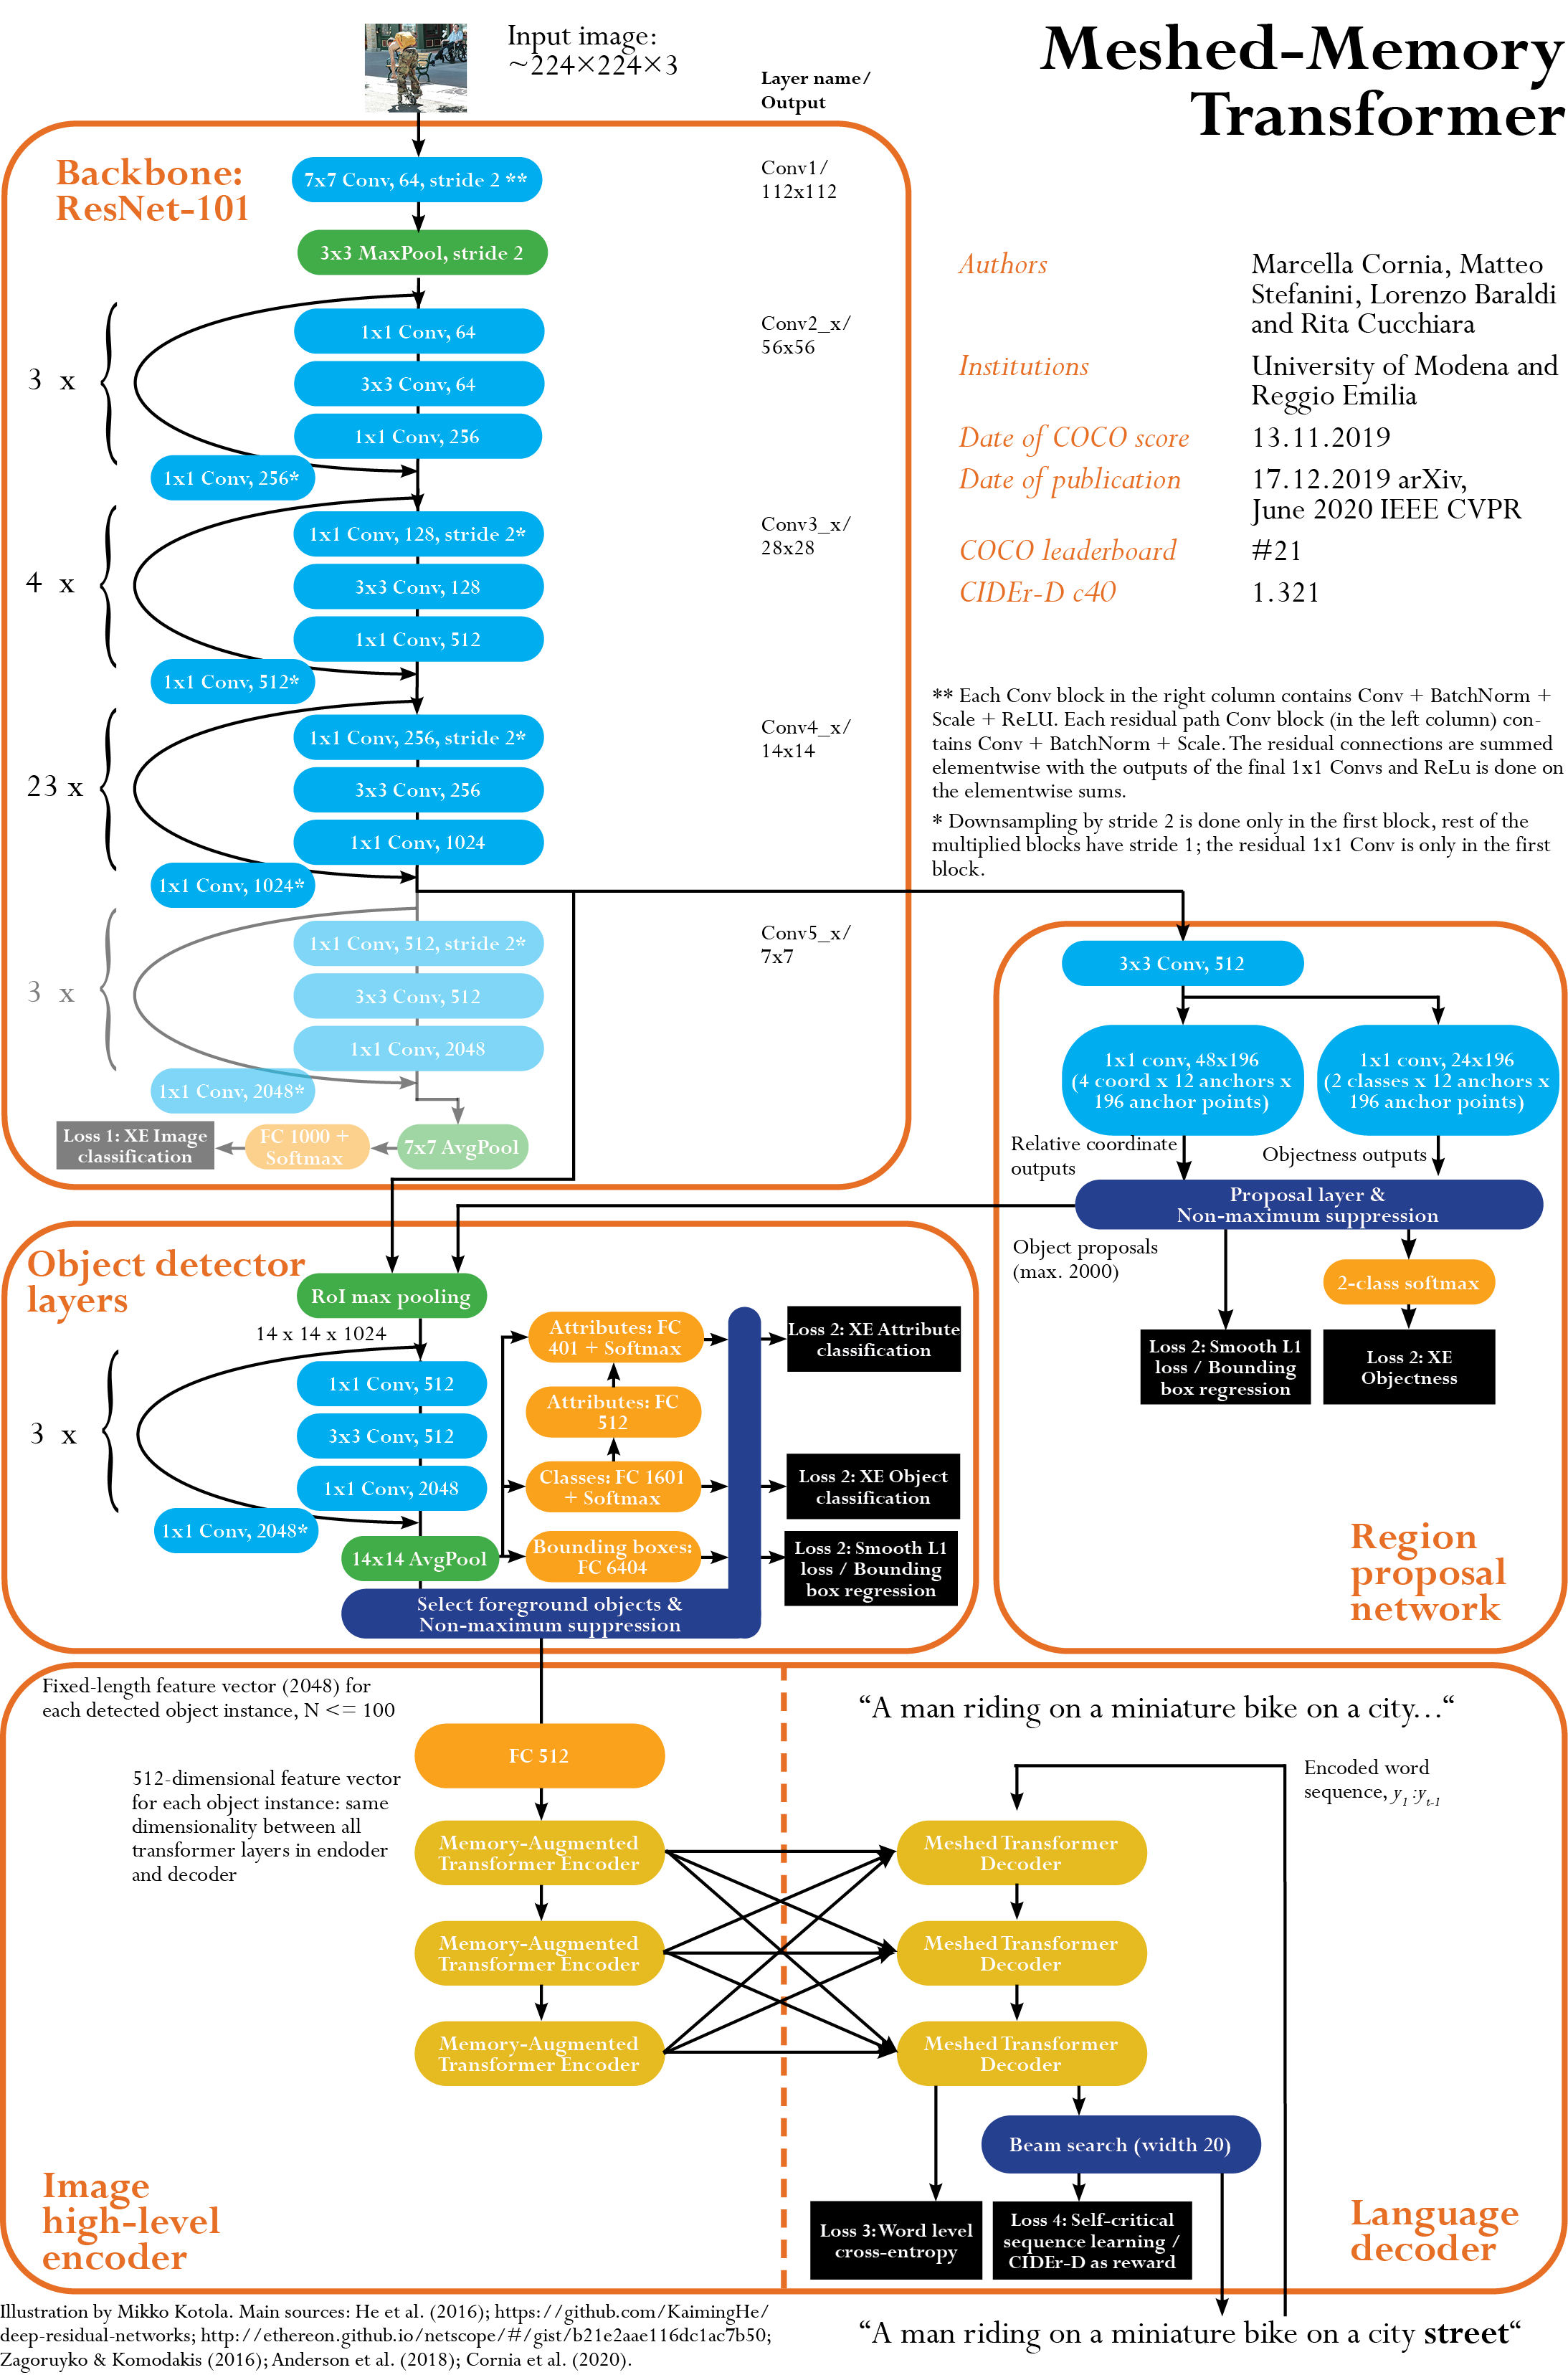
\includegraphics[width=1.0\textwidth]{./images-indesign/Architecture_M2.png}
\caption{Architecture of the complete Meshed-Memory Transformer system.}
\label{fig:architecture_M2} 
\end{figure}

\section{Meshed-Memory Transformer}
\label{section:Meshed-Memory_Transformer}
Cornia et al.~\cite{M2} present the Meshed-Memory Transformer ($\mathcal{M}^2$) model, which uses several transformer-based blocks to encode a multi-level representation of the relationships between detected objects, and then uses mesh-like connections between the encoder and the also transformer-based decoder to exploit both low- and high-level features when generating captions. Additionally, the encoder is augmented with memory, effectively leading the encoder to generalize and learn representations that are useful across images. The architecture of the $\mathcal{M}^2$ encoder-decoder is shown in figure \ref{fig:architecture_sub_M2}, and the architecture of the whole Meshed-Memory Transformer captioning system is presented in figure \ref{fig:architecture_M2}. The Meshed-Memory Transformer is currently \#21 on the COCO leaderboard, with CIDEr-D c40 score of 1.321. At the time of its testing on the evaluation server (November 13th 2019), it was ranked \#1 on the leaderboard.

\begin{figure}[h] 
\centering
\includegraphics[width=1.0\textwidth]{./images/M2_architecture.png}
\caption{Architecture of the high-level image encoder and decoder. AddNorm operations are not shown in the image to make the image more understandable. Image source: Cornia et al.~\cite{M2}.}
\label{fig:architecture_sub_M2} 
\end{figure}

\textbf{Object detection.} Just like AoANet, The $\mathcal{M}^2$ model relies on object detections and their feature vectors from the Bottom-Up Top-Down~\cite{BottomUp} model, meaning the backbone of the object detector is ResNet-101~\cite{ResNet}, there is a region proposal network to select the object areas, and a set of object detection layers. The high-level image encoder takes as input 1 to $n$ feature vectors of dimension $2048$, one for each detected object instance in the image. The Bottom-Up model outputs a maximum of 100 object instances per image, so that is the practical upper limit for $\mathcal{M}^2$ also. The proper domain training and enrichment of the feature vectors done by Anderson et al.~\cite{BottomUp} is central to the quality of the method as a whole.

\textbf{Memory vectors.} The two unique contributions of the model are usage of persistent memory vectors in the image encoder blocks, and the mesh-like connections between encoder and decoder blocks, with a learnable gating mechanism. The role of the persistent memory vectors in the encoder blocks is, according to the authors, learning and encoding \textit{a priori} knowledge~\cite{M2}. The use of the term \textit{a priori} is perhaps somewhat misguided, since the term is usually used to refer to purely analytical knowledge, knowledge which is independent of experience. What is meant by the term in this context is that the memory vectors encode features which are independent of the \textit{current} input image. The encoded information is learned from the training images during the training phase, when the parameters of the memory vectors are trained using backpropagation. But during inference, the weights of the memory features do not depend on the input image - their role is to act as additional, general keys and values within the encoder blocks. In the ablation study~\cite{M2supplement}, different amounts of parallel memory vectors, from 0 to 80, are compared. Best performance is reached with 40 memory vectors, increasing the CIDEr score from 129.4 with no memory to 131.2 with 40 memory vectors. This memory technique within a transformer-based encoder block appears generalizable, and could benefit also other models. 

\textbf{Meshed connections between encoder and decoder.} The mesh-like connections between encoder and decoder blocks is a very interesting contribution from the architecture perspective. The connections enable the system to exploit both low-level and high-level features in generating the caption, in practice learning to focus attention on single objects or their features, and the connections between objects and higher level image context, based on the language decoder state. Through an ablation study~\cite{M2}, it is shown that using 1-to-1 connections (highest encoder layer to highest decoder layer, lowest encoder layer to lowest decoder layer), in comparison to only connecting the highest encoder layer to the lowest decoder layer like in the original transformer model~\cite{Attention}, already improves the CIDEr score from 123.6 to 129.2. The meshed connections with learnable gating using sigmoid activation functions further improve the CIDEr score from 129.2 to 131.2. This mesh-based architectural pattern is likely generalizable and can benefit also other transformer encoder-decoder captioning models. The mesh connections with learnable gating can be seen as an extension of the Attention on Attention~\cite{AoA} method, and the authors of $\mathcal{M}^2$ are aware of AoA's proven benefits.

\textbf{Stacking of encoder and decoder blocks.} The $\mathcal{M}^2$ model uses three layers of encoder blocks and three layer of decoder blocks. Cornia et al. report experimenting with 2, 3 and 4 layers of encoder and decoder layers~\cite{M2supplement}, and also comparing three- and six-layered versions that use simplified transformer encoder blocks (in practice using the original transformer blocks by Vaswani et al.~\cite{Attention}). They reach best results with the three-layered version. Their hypothesis is that three layers are optimal in the captioning setting, due to the relatively low semantic complexity of sentences and the relatively small size of the training set in comparison to machine translation, where six-layer models were used~\cite{M2}.   

\textbf{Training.} The $\mathcal{M}^2$ model is trained in two phases. The main training phase is supervised learning, and uses word-level cross-entropy loss to learn to output the next word of the caption using the previous words from the ground truth caption. As the ground truth captions are fully available, the computation of all words in an output sequence (image caption) can be done in a single pass, with all operations done in parallel. The second phase of the training fine-tunes the sequence generation using reinforcement learning with the CIDEr-D as the optimization objective. In practice, it is done using the self-critical sequence training approach~\cite{SelfCriticalTraining} and beam search.

A visualization of the training process of the whole $\mathcal{M}^2$ image captioning system is shown in figure \ref{fig:training_M2}. All leading image captioning systems use a similar 3-stage training process. In the first phase the backbone network (ResNet-101) is trained on ImageNet-1k using single-label image classification loss. At this phase, the backbone learns the lower-level features of objects in images and higher-level features that enable identifying it as a representative of some object class. In the second phase, the object detector (Faster R-CNN with Bottom-Up detailed features) is trained using the Visual Genome dataset. There are a total of five loss functions in this stage (see a more detailed picture in figure \ref{fig:architecture_M2}). In the region proposal network, there are loss functions for bounding box regression (where the anchor box is located in relation to an anchor) and objectness (is there a foreground object present in the anchor box or not). In the object detection layers, the final layers of the ResNet-101 are taken as a starting point, and are further trained at this stage using three loss functions: one for object classes, a second for object features and a third for the bounding box size and location. After the second stage of training, the object detector is fully trained and can output 2048-dimensional feature vectors for each detected object region in the image. The feature vectors contain information not just related to the object classes, but also their more detailed features and interrelations, thanks to the object detector being trained on the rich Visual Genome dataset. In the third stage of training only the image captioner components (encoder and decoder) are trained. As described above, there are two training phases in this stage, the main phase of word-level cross-entropy training, and the finetuning phase that uses reinforcement learning with the CIDEr-D as the optimization objective.

\begin{figure}[h] 
\centering
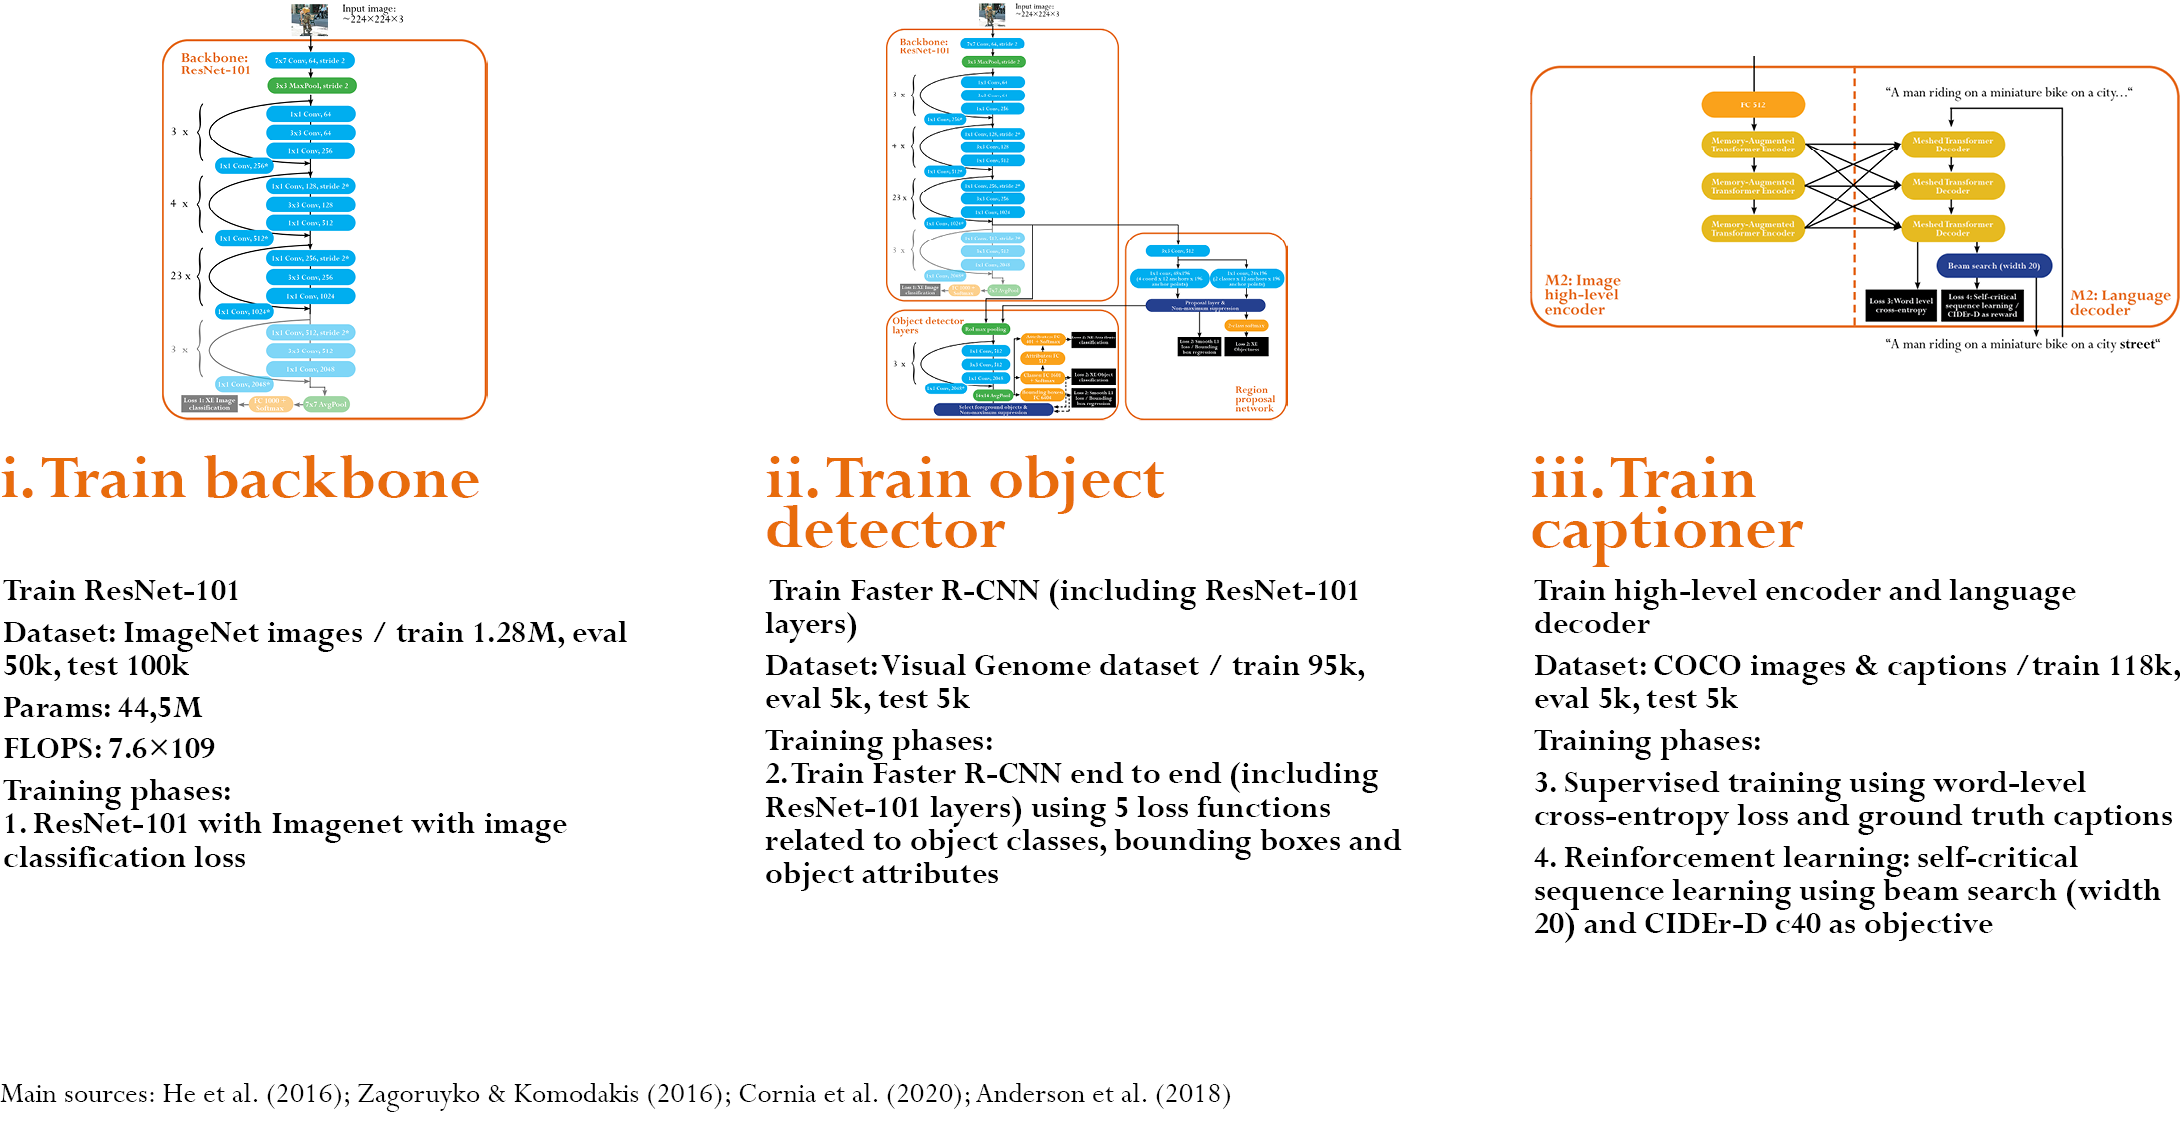
\includegraphics[width=1.0\textwidth]{./images-indesign/Training_M2.png}
\caption{Training of the whole Meshed-Memory Transformer system. The same three-stage training approach is used in all leading image captioners under investigation. The last stage has two phases, word-level cross-entropy training and sequence-level reinforcement training.}
\label{fig:training_M2} 
\end{figure}

\textbf{Main contributions.} The main contributions of the Meshed-Memory Transformer are demonstrating a fully transformer-based encoder and decoder, using persistent memory vectors in the encoder, and using mesh-like connections between the encoder and decoder blocks to enable the system to exploit both low-level and high-level features in generating the caption, The transformer-based decoder is faster to train than LSTM-based decoders due to the fact that all steps of the word-level cross-entropy training phase can be done in parallel. Also, the usage of beam search in the reinforcement learning phase and in the inference mode improves the fluency of the captions.

\pagebreak
\begin{figure}[H] 
\centering
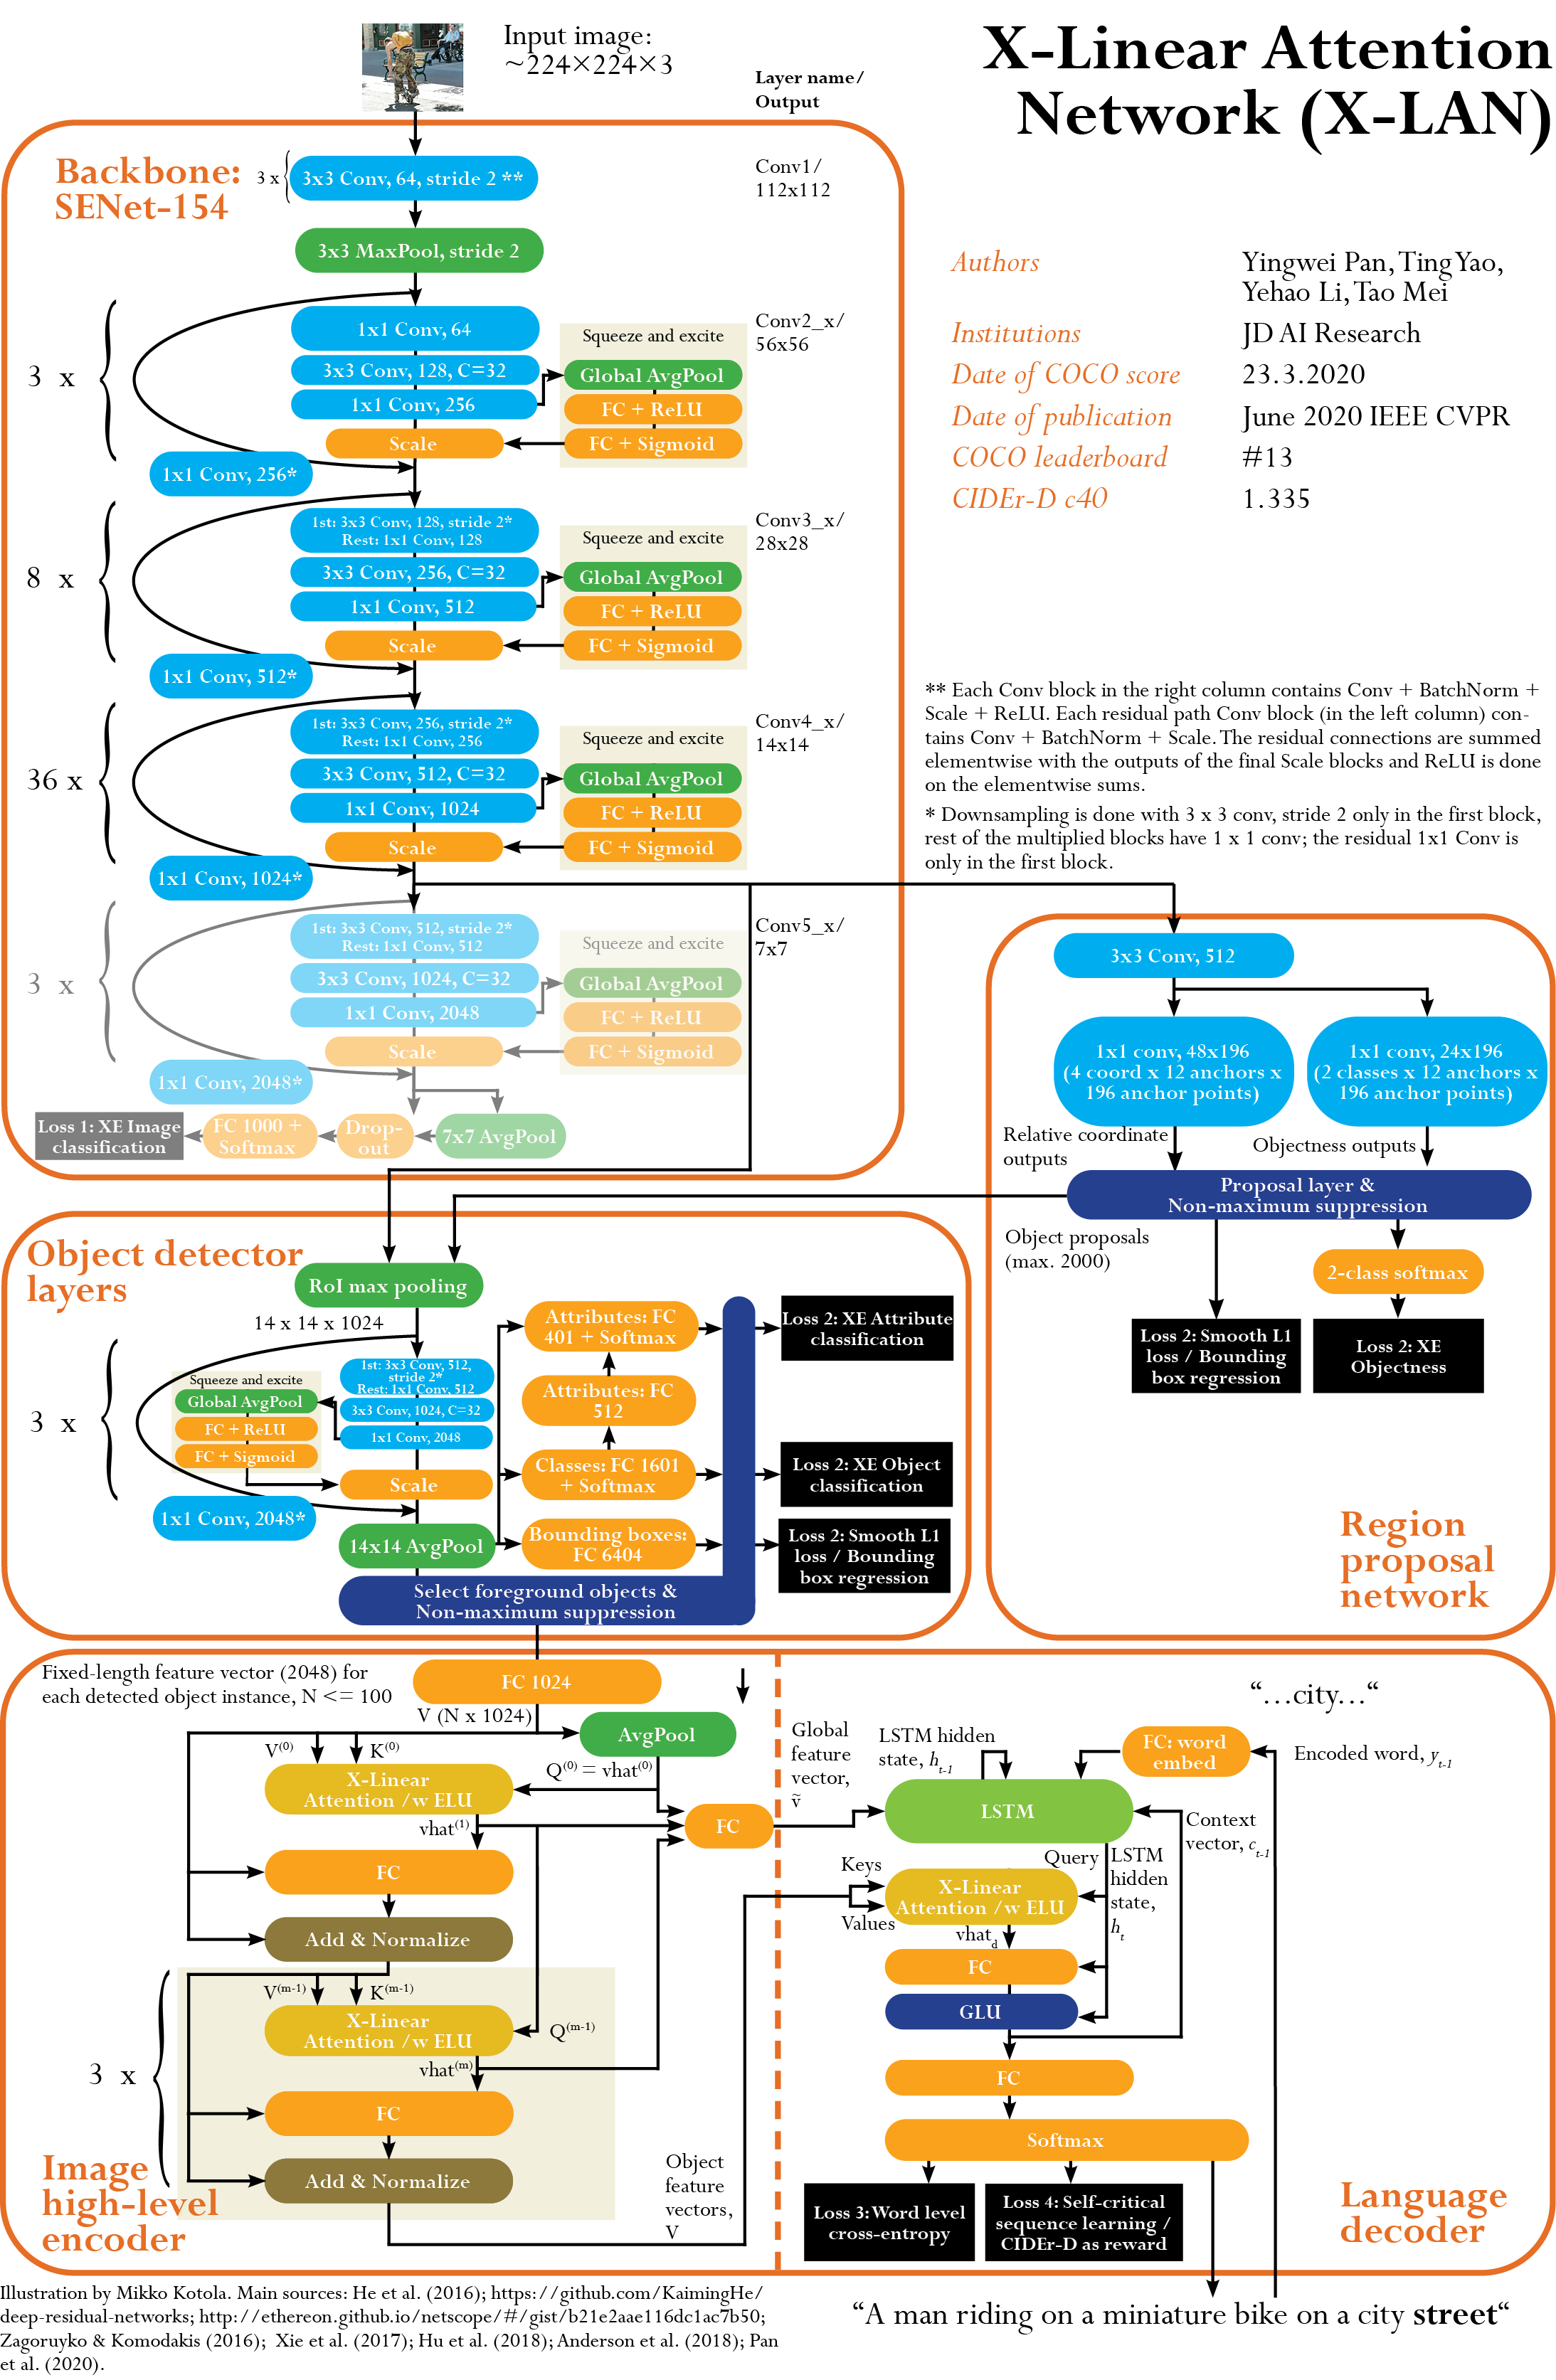
\includegraphics[width=1.0\textwidth]{./images-indesign/Architecture_X-LAN.png}
\caption{Architecture of the complete X-Linear Attention Network system. Note that the backbone is SENet-154.}
\label{fig:architecture_X-LAN} 
\end{figure}

\section{X-Linear Attention Network}
Pan et al.~\cite{XLinearAN} present a captioning model called X-Linear Attention Network. The model is based on an new, enhanced attention-based block called an X-Linear Attention (X-LA) block. X-Linear Attention seeks to take advantage of higher-order interactions both within image object detections and between the image content and natural language context. 

\begin{figure}[h] 
\centering
\includegraphics[width=0.9\textwidth]{./images/XLAN_block.png}
\caption{Architecture of the X-Linear Attention block and comparison to plain attention. The squeeze excitation route produces channel-wise attention and the softmax route produces spatial attention, meaning which refined object feature vectors to attend to. Image source: Pan et al.~\cite{XLinearAN}.}
\label{fig:XLAN_block} 
\end{figure}

\textbf{X-Linear Attention block.} X-Linar Attention uses bilinear pooling to calculate the outer product of the key and the query to take into account all pairwise interactions between the query and the key. Within the X-LA block, after bilinear pooling, two embedding layers are used to predict attention weights for each spatial region (object detection). Then softmax is used to normalize the spatial attention vector. Additionally, the embedded outer product feature map is passed through a squeeze-excitation operation to aggregate the feature map across spacial regions and produce a channel-wise attention vector. 

As visualized in figure \ref{fig:XLAN_block}, the X-Linear attention block extends the plain attention block. The main difference is using bilinear pooling to model in channel-level detail the interactions between the query $\matr{Q}$ and each key vector (transformed object detection feature vector) $\vect{k}_i$ on the one hand, and the query $\matr{Q}$ and each value vector (transformed object detection feature vector) $\vect{v}_i$ on the other. 

The initial query-key bilinear pooling is calculated 
\begin{equation}
\matr{B}_i^k = \text{ReLU}(\matr{W}_k \vect{k}_i) \odot \text{ReLU}(\matr{W}^k_q \matr{Q})
\end{equation}
%
where $\matr{W}_k \in \mathbb{R}^{D_B \times D_k}$ and $\matr{W}^k_q \in \mathbb{R}^{D_B \times D_q}$ are learnable embeddings, ReLU is the standard rectified linear unit activation ($\text{ReLU}(x) = \text{max}(0,x)$) and $\odot$ is element-wise multiplication. The learned bilinear query-key representation $\matr{B}_i^k$ carries the second order feature interactions between query and the key matrix.

$\matr{B}_i^k$ is then used to calculate the attention between the bilinearly transformed keys by using two embedding layers and a softmax for normalization:
\begin{equation}
\matr{B}_i^{'k} = \sigma(\matr{W}^k_B \matr{B}^k_i)
\end{equation}
\begin{equation}
\vect{b}^s_i = \matr{W}_b \matr{B}^{'k}_i
\end{equation}
\begin{equation}
\matr{\beta}^s = \text{softmax}(\vect{b}^s)
\end{equation}
%
where $\matr{B}_i^{'k}$ are transformed query-key vectors, $\matr{W}^k_B \in \mathbb{R}^{D_c \times D_B}$ and $\matr{W}_b \in \mathbb{R}^{1 \times D_C}$ are embeddings. Each element $\matr{\beta}^s_i$ in $\matr{\beta}^s$ is the normalized spacial attention weight for each key/value pair.

To calculate the channel-wise attention $\matr{\beta}^c$, the transformed query-key vectors $\matr{B}^{'k}_i$ are first average-pooled over all $N$ object detections to get a global channel descriptor $\bar{\matr{B}}$:
\begin{equation}
\bar{\matr{B}} = \frac{1}{N} \sum_{i=1}^N \matr{B}^{'k}_i
\end{equation}
%
Then an excitation operation, self-gating with a sigmoid, is used to calculate channel-wise attention distribution $\matr{\beta}^c$:
\begin{equation}
\matr{\beta}^c = \sigma(\matr{W}_e \bar{\matr{B}})
\end{equation}
%
where $\matr{W}_e \in \mathbb{R}^{D_B \times D_C}$ is an embedding matrix.

On the value branch of the process, the interaction of the values and queries are modeled using bilinear pooling:
\begin{equation}
\matr{B}_i^v = \text{ReLU}(\matr{W}_v \vect{v}_i) \odot \text{ReLU}(\matr{W}^v_q \matr{Q})
\end{equation}
%
where $\matr{W}_v \in \mathbb{R}^{D_B \times D_v}$ and $\matr{W}^v_q \in \mathbb{R}^{D_B \times D_q}$ are embedding matrices.

Finally the enhanced value vectors $\matr{B}_i^v$ are summed with spatial attention vectors $\matr{\beta}^s$ and then multiplied element-wise with the channel-wise attention distribution to get the final attended feature vectors:
\begin{equation}
\hat{\vect{v}} = F_\text{X-Linear}(\matr{K}, \matr{V}, \matr{Q}) = \matr{\beta}^c \odot \sum_{i=1}^N \matr{\beta}^s_i \matr{B}^v_i
\end{equation}

In order to learn higher-order interactions, X-LA blocks are extended with Exponential Linear Unit (ELU)~\cite{ELU} nonlinearity within the bilinear pooling component~\cite{XLinearAN}. This approach is argued to reduce the need to stack large numbers of X-LA block to model higher-order interaction between the input object instance feature vectors. The ELU-augmented version of the X-LA block is visualized in figure \ref{fig:XLAN_with_ELU}.

\begin{figure}[h] 
\centering
\includegraphics[width=0.8\textwidth]{./images/XLAN_with_ELU.png}
\caption{Architecture of the X-Linear attention block with Exponential Linear Unit (ELU) nonlinearity. The ELU-variant can approximately model infinity order feature interactions between inputs. Image source: Pan et al.~\cite{XLinearAN}.}
\label{fig:XLAN_with_ELU} 
\end{figure}

\textbf{X-Linear Attention Network.} X-Linear Attention blocks are used in an LSTM-based image captioning network to build an X-Linear Attention Network (X-LAN) model~\cite{XLinearAN}. The architecture of the whole X-LAN image captioning system is shown in figure \ref{fig:architecture_X-LAN}. Again, the method relies on the Bottom-Up Top-Down object detections and features as input into the image captioner. The 2048-dimensional object feature vectors are transformed to 1024-dimensional vectors. This dimensionality is then used between the encoder and decoder blocks. Within an X-LA block, the bilinear query-key representation is 1024-dimensional and the transformed bilinear query-value is 512-dimensional. Four stacked X-Linear Attention blocks with ELU are used in the high-level image encoder to learn a set of enhanced region-level and image-level features (see figure \ref{fig:architecture_X-LAN}). Each X-LA block takes the attended feature vector $\hat{\vect{v}}^{(m-1)}$ of the previous block as the input query $\matr{Q}^{(m-1)}$. In addition to the query, also the input keys $\matr{K}^{(m-1)} = \{\vect{k}_i^{(m-1)}\}_{i=1}^N$ and input values $\matr{V}^{(m-1)} = \{\vect{v}_i^{(m-1)}\}_{i=1}^N$ are taken from the output of the previous block. In each block, there is a fully connected embedding layer and an add and normalize layer to update the keys and values.
\begin{equation}
\hat{\vect{v}}^{(m)} = F_\text{X-Linear}(\matr{K}^{(m-1)}, \matr{V}^{(m-1)}, \hat{\vect{v}}^{(m-1)})
\end{equation}
%
\begin{equation}
\vect{k}_i^{(m)}= \text{LayerNorm}(\sigma(\matr{W}^k_m[\hat{\vect{v}}^{(m)}, \vect{k}^{(m-1)}]) + \vect{k}^{(m-1)})
\end{equation}
%
\begin{equation}
\vect{v}_i^{(m)}= \text{LayerNorm}(\sigma(\matr{W}^v_m[\hat{\vect{v}}^{(m)}, \vect{v}^{(m-1)}]) + \vect{v}^{(m-1)})
\end{equation}
%
where $\matr{W}^k_m$ and $\matr{W}^v_m$ are embedding matrices.

It is important to observe that the initial query $\hat{\vect{v}}^{(0)}$ is calculated by average pooling all the input object detection feature vectors. This vector is a global feature vector, carrying all the features present in the detected object areas in a condensed form. At each block, another higher-level global feature vector $\hat{\vect{v}}^{(m)}$ is calculated. These five global feature vectors (the initial $\hat{\vect{v}}^{(0)}$ and one from each encoder block) are concatenated and transformed using a fully connected layer into a final global image-level feature vector $\tilde{\vect{v}}$:
\begin{equation}
\tilde{\vect{v}} = \matr{W}_G [\hat{\vect{v}}^{(0)}, \hat{\vect{v}}^{(1)},\text{...},\hat{\vect{v}}^{(m)}]
\end{equation}
%
where $\matr{W}_G$ is an embedding matrix. The global feature vector is one of the two inputs into the decoder. The other input into the decoder is the set of refined object feature vectors $\matr{V}$ that is output from the final encoder block.

On the decoder side, an LSTM takes as input the global feature vector $\tilde{\vect{v}}$, the current input word $\vect{w}_t$, the previous LSTM hidden state $\vect{h}_{t-1}$ and the previous context vector $\vect{c}_{t-1}$. Then the output of the LSTM $\vect{h}_t$ is used as the query input into an X-LA with ELU block, and the enhanced object feature vectors $\matr{V}$ are used as keys and values. The output of the X-LA block $\hat{\vect{v}}_{d}$ is concatenated and embedded with the LSTM hidden state $\vect{h}_t$ using a fully connected layer, and the result is again concatenated with $\vect{h}_t$ and fed into a Gated Linear Unit (GLU). The output from the GLU is the context vector. The context vector $\vect{c}_{t}$ is then fed into a fully connected layer and softmax over the vocabulary is used to predict the next word to output. The context vector is also fed back to the LSTM as input to the next time step (to predict the next word in the caption).

The role of the  X-Linear Attention block with ELU in the decoder is to explore the higher-order inter-modal interactions between visual content and natural language context to boost caption generation. 

\textbf{Training.} The X-LAN model does not introduce new innovations in the training procedure, and follows the already previously described practice of two-phase training of the image captioner components. The main training phase is supervised learning with word-level cross-entropy loss, and the second phase is reinforcement learning with the CIDEr-D as the optimization objective using the self-critical sequence training approach.

\textbf{Variations of the backbone and image captioner network.} Pan et al.~\cite{XLinearAN} conduct experiments with two different backbone CNNs, the traditional ResNet-101 and SENet-154. SENet-154~\cite{SENet} is explained in detail later, in section \ref{section:SENet}. The results show that SENet-154 brings improvements to the CIDEr-D score: for the X-LAN the backbone change improves CIDEr-D from 1.303 to 1.328, and for the X-Transformer from 1.314 to 1.335. This in an important result and supports the hypothesis that utilizing innovations in the backbone and object detection networks can bring improvements to the image captioning systems as a whole. The original LSTM-based X-Linear Attention Network achieves high scores on the COCO online server, but  X-LA blocks are also integrated into a transformer-based captioner to demonstrate the generalizability and further improve the CIDEr-D score. The usage of a transformer-based image captioning network over an LSTM-based on top of the SENet-154 backbone brings a modest, likely not statistically significant, improvement of 0.007 points, from 1.328 to 1.335. The complete architecture of an LSTM-based X-Linear Network with a SENet-154 backbone is shown in figure \ref{fig:architecture_X-LAN}. Note that the architecture figure shows the LSTM-based version, while the listed X-LAN CIDEr-D score is for the transformer-based version. 

\textbf{Main contributions.} The most important contribution of the X-Linear Attention Network is the enhanced X-Linear Attention block, which can model interdependencies both within the object feature vectors and between the object features and the language context. The other contribution is showing that changing backbone CNNs can improve system performance. Usage of the Exponential Linear Unit in the encoder to model higher-order interactions and the Gated Linear Unit in the decoder are also distinctive choices in relation to the other image captioners under investigation.

\pagebreak
\begin{figure}[H] 
\centering
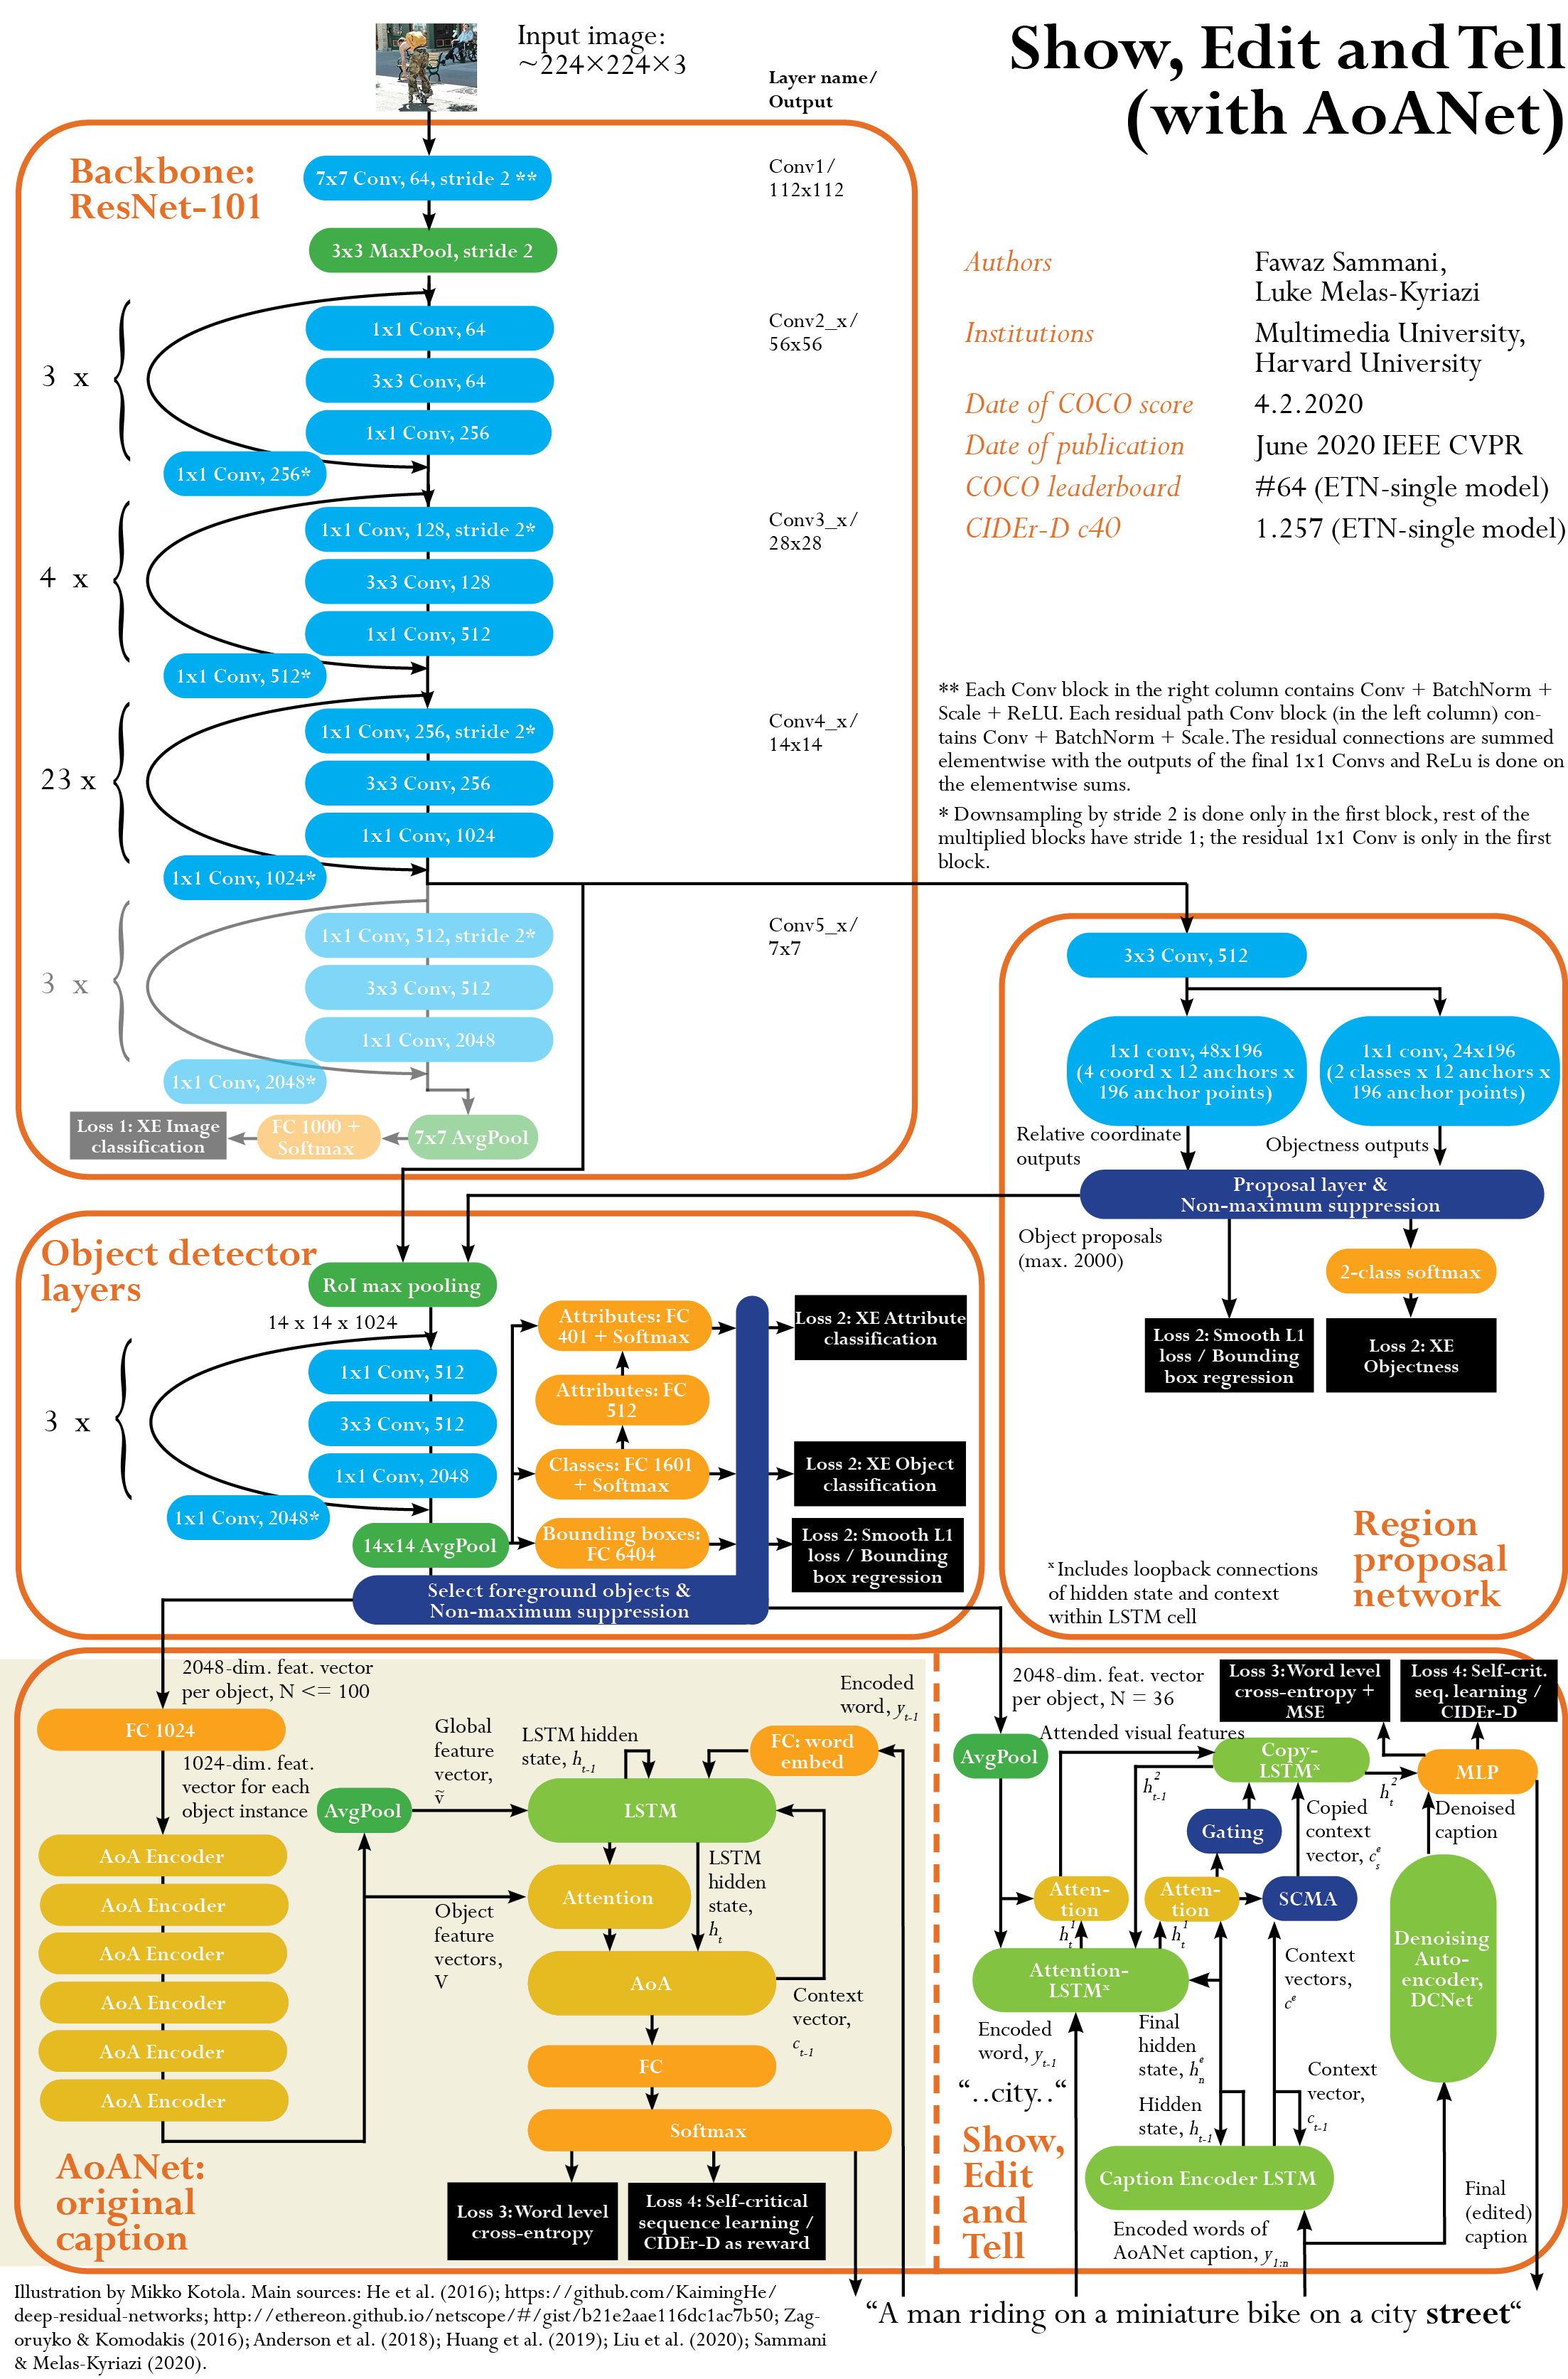
\includegraphics[width=1.0\textwidth]{./images-indesign/Architecture_ShowEdit.png}
\caption{Architecture of the complete Show, Edit and Tell system. This is the version reported in the COCO online test server leaderboard, that uses AoANet as primary captioner.}
\label{fig:architecture_ShowEdit} 
\end{figure}

\section{Show, Edit and Tell}
Sammani and Melas-Kyriazi~\cite{ShowEdit} approach the captioning task from a quite different direction than the other leading captioners. Instead of focusing on how to generate a final caption directly from the NLG decoder, they focus on iterative adaptive refinement of an existing caption. The iterative editing approach is used in other NLG tasks such as sequence-to-sequence and data-to-text generation~\cite{ShowEdit, datatotext}, but is not commonly utilized in leading image captioners. The approach aims to improve on the errors, where a captioner produces incorrect, inconsistent, or repetitive content. It does this by adding two new modules to any existing captioner to refine a caption through iterative editing. The new editing modules are directly compatible with any captioner. The added modules are EditNet, an LSTM- and attention-based network for adaptively copying data from the input caption, and DCNet, an LSTM-based denoising autoencoder. The version submitted to the COCO challenge uses AoANet as the primary captioner, and further edits the captions produced by AoANet. The architecture of the whole Show, Edit and Tell image captioning system is presented in figure \ref{fig:architecture_ShowEdit}. Notable is that the Show, Edit and Tell part of the system takes as input the image features output by the Bottom-Up object detector, and uses the precalculated features with a fixed number of object detections (36).

The CIDEr-D c40 score of Show, Edit and Tell (ETN-single\_model) on the COCO online test server does not exceed those of the other networks under investigation. Part of the score is explained by the Show, Edit and Tell model being submitted as a single model, whereas the four other captioners report their highest score for an ensemble of four models. However, even in the reported offline evaluation CIDEr scores on the Karpathy test split, the Show, Edit and Tell only matches AoANet's scores, but does not exceed them.

\begin{figure}[h] 
\centering
\includegraphics[width=0.8\textwidth]{./images/ShowEdit_idea.png}
\caption{The Show, Edit and Tell network takes as input a generated caption. At each decoding time step, the system generates attention weights (grey) indicating the importance of each word in the existing caption for the current word in the new caption. A selective copy memory attention (SCMA) operation is used to select the most likely word and directly copy its LSTM memory state to the Copy-LSTM. The new caption is then generated using the Copy-LSTM state. Image source: Sammani and Melas-Kyriazi~\cite{ShowEdit}.}
\label{fig:ShowEdit_example} 
\end{figure}

One type of mistake the editing approach proposes to fix is repetition of same nouns in the caption several times. An example of this kind of mistake is given in figure \ref{fig:ShowEdit_example}. Here, AoANet has output a caption "A sandwich on a table with a table.", mistakenly repeating the noun "table". The sentence structure of the caption is fluent, but the latter noun is not correct. A caption-editing model should be able to recognize the noun repetition and modify the caption to be something like "A sandwich on a table with a glass of wine".

\textbf{EditNet.}
EditNet~\cite{ShowEdit} is a model that is taught to copy or edit each word in an input caption. The caption is first encoded using a unidirectional
one-layer LSTM (dashed red box in figure \ref{fig:ShowEdit_architecture_sub}, which shows the EditNet components in detail). The encoded input caption $\bar{\vect{h}}_s = \left[ \vect{h}^e_1,  \vect{h}^e_2, \text{...}, \vect{h}^e_n \right]$ contains $n$ tokens, where $n$ equals the number of words in the input caption. The Attention-LSTM takes as input the concatenation of the word embedding vector $\vect{y}_{t-1}$ (marked $x$ in figure \ref{fig:ShowEdit_architecture_sub}), the last hidden state of the caption encoder $\vect{h}^e_n$, the mean-pooled image features $\bar{\vect{v}} = \frac{1}{k} \sum_i \vect{v}_i$, and the previous hidden state of the language
LSTM $\vect{h}^2_{t-1}$:
\begin{equation}
\vect{x}^1_t = [\matr{w}_t; \vect{h}^e_n; \bar{\vect{v}}; \vect{h}^2_{t-1}]
\end{equation}
%
The output of the attention LSTM $\vect{h}^1_t$ is then used to calculate one attention vector over the visual features (red arrow in figure \ref{fig:ShowEdit_architecture_sub}) and another attention vector over the textual features (blue arrow in figure \ref{fig:ShowEdit_architecture_sub}). The two attention vectors are fused with a gating mechanism and input to the Copy-LSTM. The attention weights over textual features are also used as input $\vect{\alpha}_p$ to the Selective Copy Memory Attention (SCMA) module. The role of the SCMA module is to learn to select and copy states from the input caption LSTM. The SCMA does this by measuring the similarity between $\vect{h}^1_t$ and and each word in the previous caption $\bar{\vect{h}}_s$: 
\begin{equation}
\vect{\alpha}_p = \text{softmax} (\matr{W}^T_a \text{tanh} (\matr{W}_s \bar{\vect{h}}_s + \matr{W}_h \vect{h}^1_t)
\end{equation}
%
where $\matr{W}^T_a$, $\matr{W}_s$ and $\matr{W}_h$ are embedding matrices and tanh is the hyperbolic tangent function. The SCMA then picks the word with the highest softmax output\footnote{Details on the mathematical implementation of the SCMA operation are omitted here for brevity, refer to the original paper~\cite{ShowEdit} for details.} from $\alpha_p$ (implying highest similarity to the hidden state of the Attention LSTM and therefore the word being currently generated in the language model), and copies the corresponding memory state $\vect{c}^e_t$ from the input caption encoder.

The output of the SCMA $\vect{c}^e_s$ is used as one input into the Copy-LSTM. The Copy-LSTM is an LSTM cell with an added adaptive copy mechanism. It includes a copy gate that controls how much information is taken from the SCMA module ($\vect{c}^e_s$) relative to the other input sources, the attended visual features and the hidden state $\vect{h}^1_t$. The copy gate value $c_{g_t}$ is calculated:
\begin{equation}
c_{g_t} = \sigma(\matr{W}_n \cdot [\vect{c}_t; \vect{c}^e_s])
\end{equation}
%
where $\matr{W}_n$ is an embedding matrix, $\vect{c}_t$ is the cell state vector of the LSTM, and $[;]$ is concatenation. The copy gate value is then used to calculate a modified LSTM memory state:
\begin{equation}
\vect{c}_{ap_t} = c_{g_t} * \vect{c}^e_s + (1 - c_{g_t}) * \vect{c}_t
\end{equation}
%
The hidden state is then computed with a tanh activation function of the modified memory state multiplied by the output gate:
\begin{equation}
\vect{h}^2_t = \vect{o}_t * \text{tanh} (\vect{c}_{ap_t})
\end{equation}
%
If the gate $c_{g_t}$ is 1, then the word from the input caption is copied as such, and if it is 0, then the word in the previous caption is ignored and the word is generated from scratch.

The Copy-LSTM outputs a hidden state $\vect{h}^2_t$, which is then passed to a fully connected layers (MLP in figure \ref{fig:ShowEdit_architecture_sub}) to predict the probability distribution over the vocabulary using softmax. It is also passed back to the Attention-LSTM for use in the next time step. As a final step, the probability distribution over the vocabulary is fused with the output of the denoising autoencoder to produce the output word. The embedding and hidden size of both the LSTM encoder and decoder network is 1024 and the attention dimension is 512. 

\begin{figure}[H] 
\centering
\includegraphics[width=1.0\textwidth]{./images/ShowEdit_architecture_sub.png}
\caption{The detailed architecture of the EditNet. The DCNet is marked as a single component ("De-noising Auto-encoder"). Image source: Sammani and Melas-Kyriazi~\cite{ShowEdit}.}
\label{fig:ShowEdit_architecture_sub} 
\end{figure}

\textbf{DCNet.}
Denoising autoencoders are commonly used to reconstruct noisy images. In the captioning context, the input caption is thought of as a noisy version of a true caption. DCNet\cite{ShowEdit} operates only on textual features, and is composed of a bi-directional LSTM (BiLSTM) encoder, which encodes the noisy caption into a latent representation, and an LSTM decoder, which decodes the latent representation. For the decoder, the LSTM-based Top-Down decoder (from Anderson et al.\cite{BottomUp}) is used. The encoder BiLSTM has a hidden size of 512 for each direction, and a total dimension of 1024 including both directions. The LSTM decoder has a hidden size of 1024, an embedding dimension of 1024 and an attention dimension of 512.

\begin{figure}[H] 
\centering
\includegraphics[width=0.9\textwidth]{./images/ShowEdit_architecture_sub_autoencoder.png}
\caption{The architecture of the denoising autoencoder DCNet. The noisy caption encoder is a bidirectional LSTM. The decoder consist of an Attention LSTM and a Language LSTM (typo "Langauge" is in the original image).  Image source: Sammani and Melas-Kyriazi~\cite{ShowEdit_supp}}
\label{fig:ShowEdit_architecture_sub_autoencoder} 
\end{figure}


\textbf{Training.}
Show, Edit and Tell is initially trained with the same word-level cross-entropy loss as the other captioners. Additionally, the model is optimized using an altered loss, which contains the cross-entropy loss $\mathcal{L}_{\text{XE}}(\theta)$ and a mean squared error (MSE) loss:
\begin{equation}
\mathcal{L} = \mathcal{L}_{\text{XE}}(\theta) + \mathcal{L}_{\text{MSE}}
\end{equation}

The mean squared error (MSE) is calculated between the last decoder hidden state of the language model and the last hidden state of the ground truth caption. The ground truth caption hidden state is calculated by running the ground truth caption through the encoder of the denoising autoencoder. The MSE loss is calculated using:
\begin{equation}
\mathcal{L}_{\text{MSE}} = \frac{1}{n} \sum_{i=1}^n (\vect{h}^d_n - \vect{h}^g_n)
\end{equation}
%
where the last hidden state of the language model $\vect{h}^2_n$ is linearly projected:
\begin{equation}
\vect{h}^d_n = \matr{W}_d \vect{h}^2_n + \vect{b}_d
\end{equation}
%
where $\matr{W}_d$ is an embedding matrix and $\vect{b}_d$ a bias vector.

\begin{figure}[H] 
\centering
\includegraphics[width=1.0\textwidth]{./images/ShowEdit_sample.png}
\caption{A comparison of the original caption by AoANet and the one edited by Show, Edit and Tell (ETN). The word-by-word visual attention maps of the ETN in the middle, and the textual alignment map on the right. ETN is aligning the newly generated words "top", "of", "a", "floor" to the last word in the original caption, and attending to the standing dog (and somewhat to the floor area below it) when generating these words. Image source: Sammani and Melas-Kyriazi~\cite{ShowEdit}.}
\label{fig:ShowEdit_sample} 
\end{figure}

\textbf{Main contributions.}
One main contribution of Show, Edit and Tell is taking the approach of postprocessing by editing captions and supervising their fluency and grounding in the image contents. The editing is demonstrated in practice in figure \ref{fig:ShowEdit_sample}, where Show, Edit and Tell fixes the incorrect end part of a caption generated by AoANet. The approach is unique, and some successful cases are demonstrated, but the overall performance of the model, as measured by the CIDEr score on the offline test set and the CIDEr-D score on the online test server, is only equal or even trailing to that of AoANet. The approach also adds complexity, as there are actually two captioners needed: one to generate the original caption and one to try to improve it by iterative editing. The presented editing model does not therefore deserve a named place in all future captioning systems: rather the idea of postprocessing or supervising a caption is something that can be further investigated.

\pagebreak
\begin{figure}[H] 
\centering
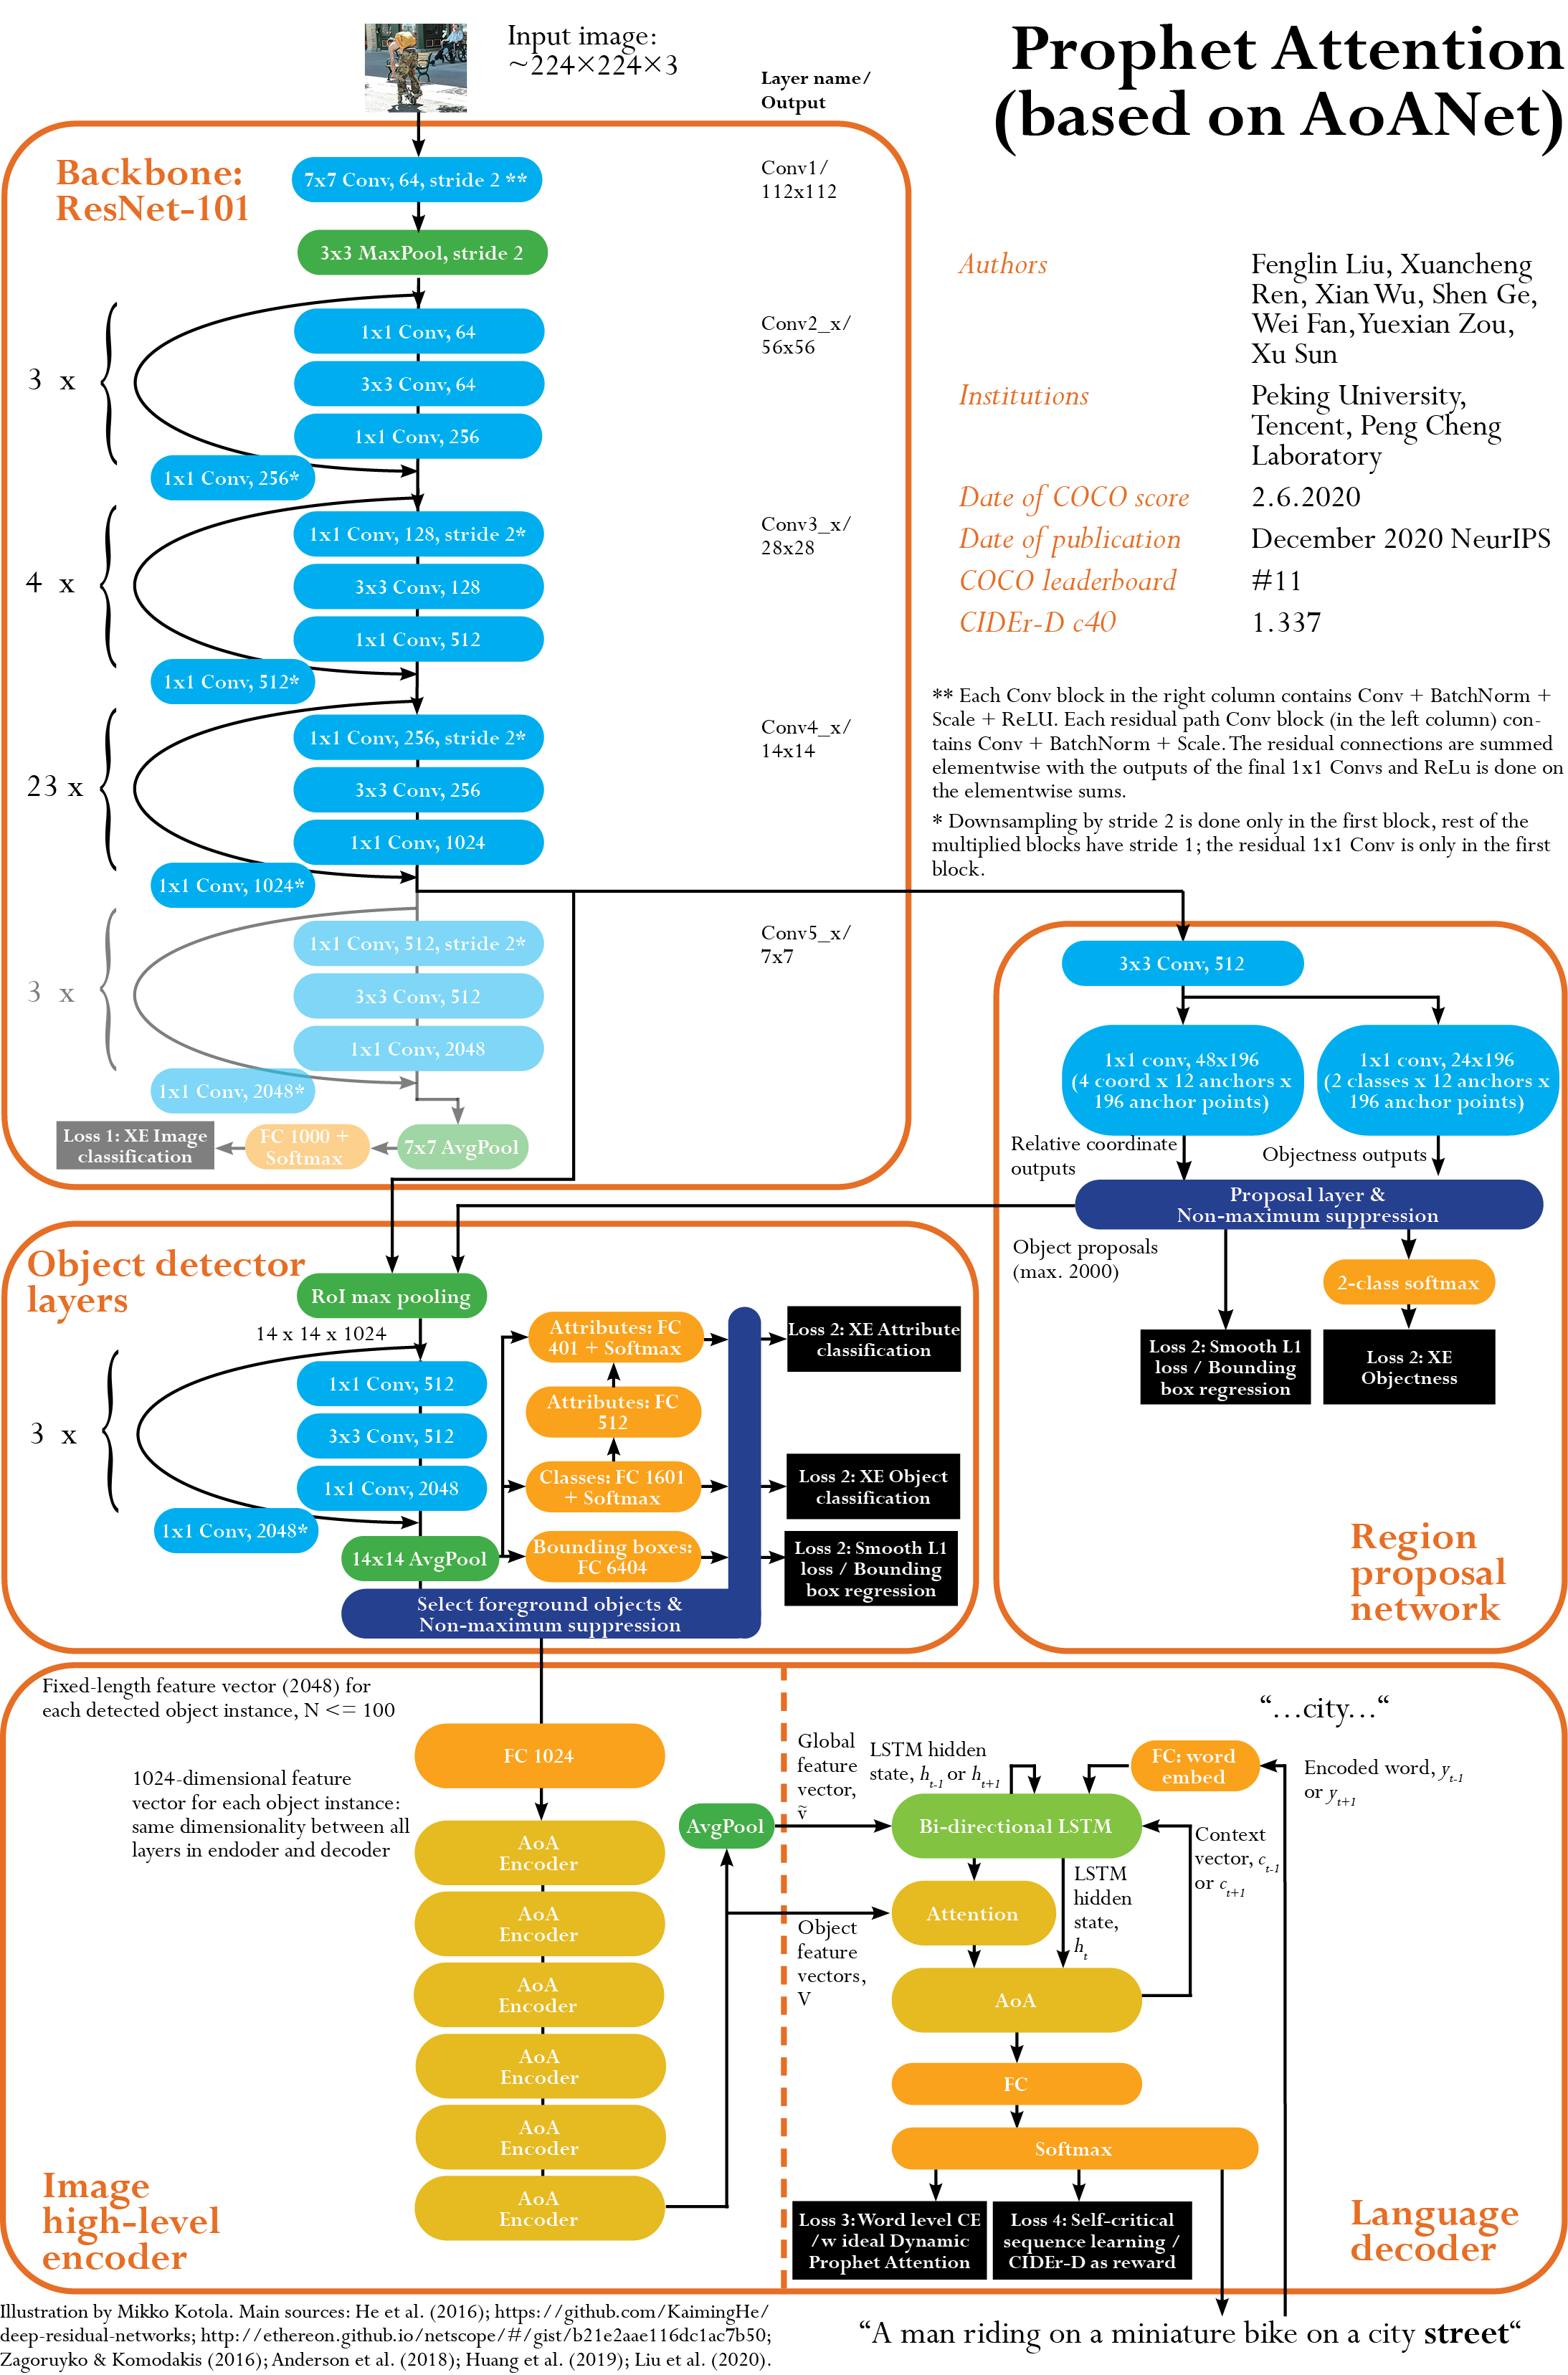
\includegraphics[width=1.0\textwidth]{./images-indesign/Architecture_Prophet.png}
\caption{Architecture of the complete Prophet Attention system. This is the version based on AoANet and reported in the COCO online test server leaderboard.}
\label{fig:architecture_Prophet} 
\end{figure}

\section{Prophet Attention}
The key idea of attention-based encoder-decoder captioners is to have the decoder attend to relevant image regions at each step of the decoding process. Liu et al.~\cite{Prophet} note that models usually use the hidden state of the current NLG input to attend to image regions, and end up attending to image regions that are related to the previous words in the caption, not the one being generated in the time-step in question. This is called the problem of \textit{deviated focus}, and it impairs the performance of both grounding the word in the image regions and as a consequence also of the whole captioning task. The Prophet Attention model aims to fix the deviated focus problem by utilizing the future information (words that come after the one currently being generated) available in the training phase to calculate ideal attention weights for image regions in the decoder. The calculated ideal weights are then used to regularize the deviated attention, grounding words in the relevant image regions.

\textbf{Deviated focus.} The deviated focus problem is demonstrated in figure \ref{fig:Prophet_problem_demo_using_AoA} using the Attention on Attention model. The model grounds each word more on regions related to the previous time steps than the current one. For example in time step 2, the model is expected to output the word "woman", but it only attends to the woman in time step 3. In time step 6, the model attends to the woman with the yellow raincoat, even if it is meant to output the word "umbrella". It attends to the umbrella only in step 7, at which point it ideally should already be attending again to the woman for outputting the word "wearing". The problem is caused by the decoder using the hidden state of the current input, already generated words, to attend to the image regions.
 
\begin{figure}[h] 
\centering
\includegraphics[width=1.0\textwidth]{./images/Prophet_problem_demo_using_AoA.png}
\caption{Deviated focus example. The image shows the Attention on Attention captioner's top 1 attended image region for each time step of the decoding process. In step 6, the model attends to the woman with the yellow raincoat, even if it is meant to output the word \textit{umbrella}. It attends to the umbrella in step 7. Image source: Liu et al.~\cite{Prophet}.}
\label{fig:Prophet_problem_demo_using_AoA} 
\end{figure}

\textbf{Prophet Attention.} Prophet Attention improves the grounding of words in more relevant image regions by calculating ideal attention weights by utilizing future information, which is readily available in the training phase~\cite{Prophet}. The ideal attention weights are then used
to guide the initial attention, which is based only on the already generated input words. The idea is to regularize the attention model based on future words.

In the regular attention approach, at each decoding time step $t$, the decoder LSTM takes as input the hidden state of the LSTM $\vect{h}_{t-1}$, and the generated word from the previous time step $\vect{y}_{t-1}$\footnote{The input word is in one-hot encoded format over the dictionary.} embedded with learnable embeddings and concatenated with the global feature vector implemented as average pooling the visual features $\bar{\vect{v}} = \frac{1}{k} \sum_{i=1}^k \vect{v}_i$~\cite{Prophet}:
\begin{equation}
\vect{h}_{t} = \text{LSTM}(\vect{h}_{t-1}, [\matr{W}_e \vect{y}_{t-1}; \bar{\vect{v}}])
\end{equation}
%
where $\vect{h}_{t}$ is the resulting hidden state of the LSTM,  $\matr{W}_e$ is a learnable word embedding matrix and $[;]$ is a concatenation operation. The LSTM output $\vect{h}_t$ is then used as a query to calculate attention scores of the relevant object feature vectors $\matr{V}$ 
\begin{equation}
\vect{\alpha}_t = f_{\text{Att}}(\vect{h}_t,\matr{V}) = \text{softmax}(\vect{w}_{\alpha} \text{tanh}(\matr{W}_h \vect{h}_t \oplus \matr{W}_V \matr{V}))
\end{equation}
%
where $\vect{w}_{\alpha}$ is an embedding vector, $\matr{W}_h$ and $\matr{W}_V$ are embedding matrices, tanh is the hyperbolic tangent function and $\oplus$ is matrix-vector addition, adding a vector to each column of a matrix. The attention scores $\vect{\alpha}_t$ are then multiplied with the object feature vectors $\matr{V}$ to generate the attended object features $\vect{c}_t$:
\begin{equation}
\vect{c}_t = \matr{V} \vect{\alpha}_t^T
\end{equation}
%
Attended object features $\vect{c}_t$ and output of the LSTM $\vect{h}_t$ are used as input to a fully connected layer and softmax to calculate probabilities of the next word over the dictionary:
\begin{equation}
\vect{y}_t = \text{softmax}(\matr{W}_p [\vect{h}_t ; \vect{c}_t] + \vect{b}_p)
\end{equation}
%
where $\matr{W}_p$ is a learnable linear transformation and $\vect{b}_p$ a learnable bias vector.
 
The approach of Prophet Attention is to augment the network in the training phase with a Bidirectional LSTM (BiLSTM) to calculate ideal attention weights $\hat{\vect{\alpha}}_t$. The whole word sequence $\vect{y}_{i:j}$ is first encoded using the BiLSTM to get $\vect{h}^{'}_{i:j}$, and then the ideal attention weights are calculated:
\begin{equation}
\hat{\vect{\alpha}}_t = f_{\text{Prophet}}(\vect{h}^{'}_{i:j}, \matr{V}) = \frac{1}{j-i+1} \sum_{k=i}^j f_{\text{Att}}(\vect{h}^{'}_k , \matr{V})
\end{equation}
%
where, $i$ is the index of the first word in the sequence and $j$ is the index of the last word, and $f_{\text{Att}}$ is the same attention function as in the mainstream attention and shares the same parameters.

\begin{figure}[h] 
\centering
\includegraphics[width=0.9\textwidth]{./images/Prophet_architecture_idea.png}
\caption{Prophet attention uses a bi-directional LSTM to calculate ideal attention weights $\vect{\hat{\alpha}}_t$ based on future words in the ground truth caption as a target for the main attention model weights $\vect{\alpha}_t$, which is based only on the previously generated words. Image source: Liu et al.~\cite{Prophet}.}
\label{fig:Prophet_architecture_idea} 
\end{figure}

\textbf{Training.} Prophet attention introduces new loss functions and changes the supervised training phase by introducing the regularization of the attention towards image features in the image decoder.

The original cross-entropy loss $\mathcal{L}_{\text{XE}}(\theta)$ is defined as:
\begin{equation}
\mathcal{L}_{\text{XE}}(\theta) = - \sum_{t=1}^T \text{log}(p_\theta(y^*_t | y^*_{1:t-1}))
\end{equation}
%
where $y^*_t$ is a word at time-step $t$, and $p_\theta(y^*_t | y^*_{1:t-1})$ is the probability of a word conditional to the previously generated words in the sequence. To take the ideal losses into account during training, a regularizing loss function that uses the L1 norm to penalize deviation of predicted attention scores $\vect{\alpha}_t$ from the ideal attention scores $\hat{\vect{\alpha}}_t$ is introduced:
\begin{equation}
\mathcal{L}_{\text{Att}}(\theta) = - \sum_{t=1}^T {\lVert}\vect{\alpha}_t - \hat{\vect{\alpha}}_t{\rVert}_1
\end{equation}
%
The full training objective loss function function $\mathcal{L}_{\text{Full}}(\theta)$ is then defined as:
\begin{equation}
\mathcal{L}_{\text{Full}}(\theta) = \mathcal{L}_{\text{XE}}(\theta) + \hat{\mathcal{L}}_{\text{XE}}(\theta) + \lambda \mathcal{L}_{\text{Att}}(\theta)
\end{equation}
%
where $\lambda$ is a hyperparameter to control the amount of regularization. Based on experiments, $\lambda$ value of $0.01$ gives the best overall results for the AoANet-based Prophet network.

In the supervised training phase, the captioner is first trained without the Prophet part, only using $\mathcal{L}_{\text{XE}}(\theta)$, for a number of epochs (25 in the paper) to initialize the decoder parameters. Then supervised training is continued using the full loss function $\mathcal{L}_{\text{Full}}(\theta)$. The self-critical reinforcement training phase with CIDEr-D as the optimization objective is used similarly as described in the other models under investigation. As the Prophet Attention is only used in the training phase to guide the attention, the inference stage, where the future words are naturally not available in any case, works precisely as before - the learned weights just guide the decoder to attend to more relevant image features. 

\textbf{Dynamic Prophet Attention.} Dynamic Prophet Attention (DPA)~\cite{Prophet} is a practical refinement of the Prophet Attention approach to account for there being different kinds of words in the captions. DPA takes into account noun phrases (NP)\footnote{The spaCy library is used for noun phrase tagging in the original Prophet implementation.} (for example "a yellow umbrella"), non-visual words (NV) (for example "the" and "of") and groups all other words, such as verbs, together. For noun phrases, the prophet attention is utilized so that the ideal attention is based \textit{only} on the words in the noun phrase (be they in the past, current or future time step). For non-visual words, the Prophet-related loss functions $\hat{\mathcal{L}}_{\text{XE}}(\theta)$ and $\mathcal{L}_{\text{Att}}(\theta)$ are disabled and only the original loss $\mathcal{L}_{\text{XE}}(\theta)$ is used, meaning that the attention is based mostly on the past words. For the other words, the ideal attention is based \textit{only} on the current word.

\textbf{Generalizability.} The Prophet Attention approach is implemented on top of several LSTM-based captioners including the original Bottom-Up Top-Down captioner~\cite{BottomUp} and the AoANet. The AoANet-based Prophet network is the best version and is the one described in figure \ref{fig:architecture_Prophet} and used for the COCO online test server scores. The effect of adding the Dynamic Prophet Attention to AoANet is increasing CIDEr-D c40 from 1.296 to 1.337 points, a notable improvement. An improvement of 0.55 CIDER c40 points is also demonstrated for the Bottom-Up Top-Down network in the offline evaluation.

\textbf{Main contributions.} The main contribution is an improved approach to grounding each generated word on the most relevant image regions instead of those regions most relevant to the already generated words. The Prophet Attention approach is novel and an isolated improvement, meaning that is can be easily incorporated into any attention-based encoder-decoder captioning model. The original paper demonstrates the implementation for LSTM-based decoders, utilizing a bidirectional LSTM for the training phase. Similar approach could be implemented for transformer-based decoders. This possibility is further discussed in chapter \ref{chapter:improving_system}.

\chapter{Improving the Backbone Image Processing Network}
\label{chapter:backbone}
Object detection as a task is closely related to image classification, and both of these tasks use the same CNN-based backbone networks for the early stages of the processing. For this reason, advances in these backbone networks potentially contribute also to the performance of image captioning systems as a whole. Furthermore, most current state-of-the-art image captioners rely essentially on ResNet-101, which is already 5 years old, as used in Faster R-CNN~\cite{FasterRCNN} and Bottom-Up Top-Down~\cite{BottomUp}. Computer vision, object classification and object detection are very active areas of research. This chapter presents an overview to latest research in these areas and proposes ways to improve the backbone component. This chapter is followed up by reviewing possible improvements to the object detector components in chapter \ref{chapter:objectdetector_improvements}.

As described in chapter \ref{chapter:captioners}, X-Linear Attention Network experiments with changing the backbone network from ResNet-101 to SENet-154 and achieves improvements in the CIDEr score of the system. This demonstrates that changing backbones can improve captioning system performance. This is understandable, as the backbone is the largest part of the system, and the capacity of the backbone to learn image features that are useful in detecting objects and their attributes is central for the ability of the object detection layers, high-level image encoder and NLG decoder to detect objects, learn the interactions between the objects and the overall image context, and generate captions based on that information.

The backbones presented in this chapter were chosen based on their contribution to the accuracy of image classification or object detection. For example the Darknet~\cite{YOLO9000, YOLOv3} networks used as backbones in the YOLO family of object detectors are not presented, because their contributions are focused on efficiency of training and inference, not primarily on advancing accuracy. The first three sections, \ref{section:ResNeXt} ResNeXt, \ref{section:SENet} Squeeze-and-Excitation Networks and \ref{section:EfficientNets} EfficientNets, present central improvements to the ResNet architecture. Section \ref{section:VisionTransformers} Vision Transformers presents an alternative, transformer-based approach to backbones. Section \ref{section:LargeDatasets} discusses the role of large datasets in improving backbones, and finally section \ref{section:BackboneImprovements} draws together the most potential improvements to backbone networks.

\section{ResNeXt}
\label{section:ResNeXt}
ResNeXt~\cite{ResNeXt} evolves the ResNet architecture of repeating layers and residual connections by augmenting it with a split-transform-merge strategy. The split-transform-merge strategy comes from the Inception~\cite{InceptionV4} modules, where the input is split into a few lower-dimensional embeddings by using $1 \times 1$ convolutions, transformed by a set of specialized convolutional filters (typically $3 \times 3$ or $5 \times 5$), and finally merged by concatenation~\cite{ResNeXt}. The aim of an Inception module is to approximate the representational power of a single large layer with lower computational cost. The innovation of ResNeXt in relation to other Inception-based approaches is to keep the topology of each path constant, effectively introducing the size of the set of transformations, \textit{cardinality}, as a new dimension alongside the width and depth of a network. Moreover, it is demonstrated, that increasing cardinality is a more effective way of gaining accuracy in image classification than increasing the depth or width of a CNN. The ResNeXt block can be implemented in three equivalent ways as shown in figure \ref{fig:ResNeXt_block}. Implementation \textit{a} splits the input into 32 paths for all three convolutions and then concatenates the results together and adds them together with the residual connection. Implementation \textit{b} replaces the last $1 \times 1$ convolutions by early concatenation and one larger $1 \times 1$ convolution. This is equivalent, because the $1 \times 1$ convolution learns features channel-wise and the inputs to it are also split channel-wise in both cases. Implementation \textit{c} uses \textit{grouped convolutions}, where input and output channels are divided into
$C$ groups, and convolutions are separately performed within each group. The grouped convolutional layer performs 32 groups of convolutions, where the input and output channels for each group are 4-dimensional. The grouped convolutional layer also concatenates the outputs into a 128-dimensional concatenated output vector, which is then fed into the last $1 \times 1$ convolution. This implementation looks quite similar to the original ResNet block, but the middle convolution layer is wider and has sparser connections. 

\begin{figure}[h] 
\centering
\includegraphics[width=1.0\textwidth]{./images/ResNeXt_block.png}
\caption{Three equivalent implementations of the ResNeXt block with 256-dimensional inputs and outputs. The implementation on the right is the one used as the base for SENets. Image source: Xie et al.~\cite{ResNeXt}}
\label{fig:ResNeXt_block} 
\end{figure}

\section{Squeeze-and-Excitation Networks}
\label{section:SENet}
Squeeze-and-Excitation Networks (SENets)~\cite{SENet} seek to improve the representational power of a CNN by explicitly modeling the interdependencies between the channels of its convolutional features. SENet achieves this by introducing a mechanism to allow the network to perform feature recalibration, to enable learning to use global information to selectively emphasize informative features and suppress less informative ones. SENet contributes by augmenting the stackable block structure, so the contribution is reusable in many CNNs based on stackable blocks, including ResNet and ResNeXt.

\begin{figure}[h] 
\centering
\includegraphics[width=0.9\textwidth]{./images/SENet_squeeze_and_excitation.png}
\caption{A Squeeze-and-Excitation block. The squeeze features (produced by $\matr{F}_{\text{sq}}$) learn useful channels and are then used to excite ($\matr{F}_{\text{ex}}$) the most useful channels in the output $\matr{U}$, resulting in channel-wise scaled features $\tilde{\matr{X}}$. Image source: Hu et al.~\cite{SENet}.}
\label{fig:SENet_block} 
\end{figure}


A Squeeze-and-Excitation block is depicted in figure \ref{fig:SENet_block}. The SE block is placed after some base transformation $\matr{F}_{\text{tr}}$ such as a ResNet block. The squeeze operation $\matr{F}_{\text{sq}}$ is implemented by globally average pooling each channel. The channel descriptor statistic vector $\vect{z} \in \mathbb{R}^C$ is calculated by shrinking the input $\matr{U} \in H \times W \times C$ through spatial dimensions height $H$ and width $W$. The $c$:th element in $\vect{z}$ is
\begin{equation}
z_c = \matr{F}_{\text{sq}}(\vect{u}_c) = \frac{1}{H \times W} \sum_{i=1}^H \sum_{j=1}^W \vect{u}_c(i,j)
\end{equation}
%
The excitation operation $\matr{F}_{\text{ex}}$ is implemented by a simple gating mechanism:
\begin{equation}
\vect{s} = \matr{F}_{\text{ex}}(\vect{z}, \matr{W}) = \sigma(\matr{W}_2 \text{ReLU}(\matr{W}_1\vect{z}))
\end{equation}
%
where $\vect{s}$ is the resulting channel-wise excitation weight vector, $\sigma$ is the sigmoid function, $\matr{W}_1 \in \mathbb{R}^{\frac{C}{r} \times C}$, $\matr{W}_2 \in \mathbb{R}^{C \times \frac{C}{r}}$, and $r$ is a reduction ratio for the bottleneck in the gating. The final output of the SE block is calculated by rescaling the input $U$ with the activations $\vect{s}$:
\begin{equation}
\tilde{\vect{x}}_c = \matr{F}_{\text{scale}}(\vect{u}_c, s_c) = s_c \cdot \vect{u}_c
\end{equation}
%
where $\tilde{\matr{x}} = [\tilde{\vect{x}}_1, \tilde{\vect{x}}_2, ... , \tilde{\vect{x}}_C]$, and $s_c \cdot \vect{u}_c$ is channel-wise multiplication of the scalar scaling factor $s_c$ and the channel feature map $\vect{u}_c \in \mathbb{R}^{H \times W}$.

The squeeze-and-excitation blocks can be applied upon a ResNet architecture~\cite{SENet}. A SE-ResNet Module is depicted in figure \ref{fig:SENet_module}. The SE-block is placed after each convolutional ResNet block, before the identity branch is summed with the transformed branch. The SE-ResNet-101 is shown to outperform the plain ResNet-101 in the object detection task on the COCO dataset by improving average precision (AP) from 27.2 to 27.9. A complete SENet-154 Network architecture, based on a ResNeXt-152, is shown in the X-LAN architecture figure \ref{fig:architecture_X-LAN}.

\begin{figure}[h] 
\centering
\includegraphics[width=0.7\textwidth]{./images/SENet_ResNet_module.png}
\caption{The structure of a plain ResNet Module and a squeeze-and-excite-augmented SE-ResNet Module. Image source: Hu et al.~\cite{SENet}.}
\label{fig:SENet_module} 
\end{figure}

\section{EfficientNets}
\label{section:EfficientNets}
Already in 2016, Zagoruyko and Komodakis~\cite{ZagoruykoK16} presented \textit{Wide Residual Network} (WRN) architecture, which focused on increasing the width of a network, the number of channels in a convolutional layer, instead of depth, the number of layers. They showed that for an image classification task, a 16-layer wide network that uses residual blocks has the same accuracy as a 1000-layer thin deep network using similar blocks. Both networks have approximately the same amount of parameters, but the WRN is much faster to train. The computational efficiency of training WRNs seems to be related to GPUs being able to take advantage of efficient parallel matrix operations in wider convolution blocks, compared to a deeper network with thinner convolution blocks.

Tan and Le~\cite{EfficientNet} continue the work on ways of scaling up CNNs. They observe that convolutional networks can be scaled up by increasing their depth, width or resolution. Depth is defined as the number of layers in the network, width as the number of channels in each convolutional layer and resolution as the number of pixels in the input image. They observe that scaling up just one of these dimensions does not produce optimal accuracy, but the accuracy gain diminishes or even saturates after some point of each dimension. Instead, they propose scaling up networks by uniformly scaling all dimensions of depth, width and resolution using a compound coefficient. The compound coefficient $\phi$ is used to determine the optimal constants $\alpha, \beta, \gamma$, which control the scaling of the depth $d = \alpha^\phi$, width $w = \beta^\phi$ and resolution $r = \gamma^\phi$:
\begin{equation}
\alpha \cdot \beta^2 \cdot \gamma^2 \approx m
\end{equation}
%
where $\alpha \leq 1, \beta \leq 1, \gamma \leq 1$ and the $m$ on right side of the equation defines the multiplier of the resources that can be spent on scaling the network. 

The systematic uniform scaling approach is demonstrated to work for efficient scaling of for example ResNets, but it is also used to create a new family of convolutional networks called EfficientNets~\cite{EfficientNet}. The main building block of EfficientNets is the mobile inverted bottleneck module (MBConv) with added squeeze-and-excitation optimization. There are several innovations in the MBConv~\cite{MobileNetv2} module. Firstly, the residual connections are between the layers with fewer channels instead of the wider layers. The idea is that the bottlenecks contain all the necessary information, and the expansion layers act merely as implementation details that accompany a non-linear transformation of the tensor. The non-linearity is also removed from the bottleneck to prevent it from destroying too much information, making it a \textit{linear bottleneck}. The convolutions used in the expansion layer are \textit{depthwise separable convolutions} instead of plain convolutions. Depthwise separable convolutions replace a full convolutional operator with a factorized version that splits the convolution into two separate layers. The first layer is a depthwise
convolution, which performs lightweight filtering by applying a single convolutional filter (most often $3 \times 3$ or $5 \times 5$ in the MBConv module) per input channel. The second layer is a pointwise $1 \times 1$ convolution, which is responsible for building new features by computing linear combinations of the input channels. Depthwise separable convolutions work almost as well as standard convolutions but the computational cost is 8-9 times smaller~\cite{MobileNetv2} in the backbone network settings. After the expansion layer, features are projected back to a
low-dimensional representation using a linear ($1 \times 1$) convolution. The comparison of the structure of an MBConv block to a regular residual block is shown in figure \ref{fig:MBConv} . The MBConv module was originally invented to support efficient operations on low-resource mobile platforms, but they have since successfully been used also in large networks in high-resource environments.

\begin{figure}[h] 
\centering
\includegraphics[width=1.0\textwidth]{./images/Inverted_residual_block.png}
\caption{The traditional residual block on the left, the inverted residual MBConv block structure on the right. The main innovations in the MBConv block are connecting the low-dimensional representations by residual connections, using a linear bottleneck without non-linearity and using depthwise separable convolution in the expansion layer. The layers with diagonal markings do not use non-linearities. Image source: Sandler et al.~\cite{MobileNetv2}.}
\label{fig:MBConv} 
\end{figure}

The architecture of the smallest network of the EfficientNet family, EfficientNet-B0, is shown in figure \ref{fig:EfficientNet-B0}. It is noteworthy, that the EfficientNet architecture has relatively more layers at higher resolutions than $14 \times 14$ than the ResNet-101.

\begin{figure}[h] 
\centering
\includegraphics[width=0.7\textwidth]{./images/EfficientNet-B0.png}
\caption{The architecture of the baseline EfficientNet-B0. Resolution is the input resolution of the stage layers, and \#Layers is the number of similar layers in a stage. Image source: Tan and Le~\cite{EfficientNet}.}
\label{fig:EfficientNet-B0} 
\end{figure}

Using multiplier 2 for a small baseline EfficientNet-B0, which has 18 convolutional layers, Tan and Le use grid search and discover that the optimal scaling constants are $\alpha = 1.2, \beta = 1.1, \gamma = 1.15$. They hypothesize that these scaling constants are quite near optimal for this network architecture. Using these constants, they define EfficientNets of different sizes, from EfficientNet-B0 with 5.3M parameters and a 76.3 \% top-1 accuracy\footnote{Top-1 accuracy means that the class predicted by a model to have the highest probability is the same as the ground truth class. Sometimes also top-5 accuracy is reported. In the top-5 case it is only required that the ground truth class in the top five most probable classes as predicted by the model.} on ImageNet, all the way to EfficientNet-B7 with 66M parameters and a 84.4 \% top-1 accuracy.

A comparison of the ImageNet top-1 accuracy vs. number of parameters for several networks including EfficientNets, SENet-154, ResNeXt-101 and ResNet-152 is shown in figure \ref{fig:EfficientNet_comparison}.

\begin{figure}[h] 
\centering
\includegraphics[width=0.7\textwidth]{./images/EfficientNet_comparison.png}
\caption{EfficientNets achieve higher ImageNet top-1 accuracy than other convolutional networks with a smaller number of parameters. Image source: Tan et al.~\cite{EfficientNet}.}
\label{fig:EfficientNet_comparison} 
\end{figure}

\section{Vision Transformers}
\label{section:VisionTransformers}
Convolutional neural networks have for a long time been the leading approach in computer vision. Recently, transformer-based networks have been proposed as an alternative to CNNs also for multi-level feature learning, the essence of the backbone networks.
Dosovitskiy et al.~\cite{VisionTransformers} propose to use Vision Transformers (ViT) instead of CNNs. Vision Transformers are an adaption of transformers to the domain of computer vision. 

In Vision Transformers, the image is split into patches, and the sequence of linear embeddings of these patches is used as input to a transformer. Image patches are treated the same way as tokens (words) in the original natural language processing (NLP) related transformer model. The idea is to use the transformer model with minimal alterations in the computer vision context. The idea of the Vision Transformer is presented in figure \ref{fig:Vision_transformer}.

\begin{figure}[h] 
\centering
\includegraphics[width=1\textwidth]{./images/VisionTransformer.png}
\caption{Vision Transformer model adapts the transformer into computer vision by splitting the image into patches, adding positional encodings and a class encoding, and using them as a sequence similarly to natural language processing domain transformer models. Image source: Dosovitskiy et al.~\cite{VisionTransformers}}
\label{fig:Vision_transformer} 
\end{figure}

Vision Transformers lack some of the core features of the CNNs, namely translational equivariance and locality. For this reason, they do not reach the same image classification performance as ResNet models when trained on only the widely used ImageNet-1k dataset (1,4 million images). But when trained with a still larger dataset such as the full ImageNet-21k (14,2 M images) or JFT-300M (303 M images), the ViT is able to overcome the initial handicap and reaches state-of-the-art performance (image classification top-1 accuracy of 88.55 \% on ImageNet)~\cite{VisionTransformers}. Interestingly, the ViT models are demonstrated to learn the 2-dimensional relation of the image patches autonomously, and hybrid approaches partly using convolutional features do not improve performance when models are trained with large datasets. The ViT models are trained in a supervised fashion by adding a class embedding to the input and using the state of that embedding after the transformer encoding layers for classification.

Vision Transformers are a major breakthrough in the image processing backbone networks. Importantly, they reach higher classification accuracy than ResNet-based models and the accuracy increase that is associated with training on ever larger datasets does not saturate yet at the level of 300 million images~\cite{VisionTransformers}, suggesting that even larger datasets can further improve the performance of this type of backbone network.

Caron et al.~\cite{DINO} build on Vision Transformers and present an approach based on self-supervised learning with knowledge distillation called DINO (knowledge \textbf{di}stillation with \textbf{no} labels). \textit{Knowledge distillation} is a learning paradigm where a student network is trained to match the output of a teacher network. In DINO, the structure of the student and teacher networks is identical. Global views of an image, meaning crops covering over 50 \% of an images, are passed through the teacher and more tightly cropped local views, covering a smaller area of the image, are passed through the student. Effectively, the student is taught to model the global features of an image from cropped, local views. Interestingly, the teacher network is not pretrained, but is taught at the same time as the student network using a momentum encoder approach. 

The Vision Transformer model trained with the DINO training approach and used together with a simple k-nearest neighbours (k-NN) classifier produces a good ImageNet top-1 accuracy of 78.3 \%~\cite{DINO}. While this is clearly below the supervised ViT accuracy, the result is still good and demonstrates that a self-supervised approach can potentially reach even higher levels with more data. An additional note is that Vision Transformers do not use batch normalization, and DINO used with ViT is completely batch normalization free. I cannot go into more details of the DINO approach in this thesis -- please refer to the DINO paper for more detailed information on the approach.

Touvron et al.~\cite{DeeperImageTransformers} report a large Vision Transformer based model that achieves 86.5 \% top-1 accuracy on ImageNet\footnote{The exact model that achieves this result is $\text{CaiT-M48}\uparrow448\Upsilon$. This model has 48 self-attention blocks and 2 class attention blocks. The main training phases uses input resolution $224 \times 224$, but the model is fine-tuned with resolution $448 \times 448$ images (notated by $\uparrow448$) and uses a knowledge distillation training scheme (notated by $\Upsilon$). See details in the CaiT paper~\cite{DeeperImageTransformers}.} when training with only ImageNet-21k data (not using for example JFT-300M). This result again strengthens the position of the vision transformer approach, since the result is achieved with only the ImageNet dataset. They name their architecture Class-Attention in Image Transformers (CaiT). The main contribution is splitting the processing into two stages. The first, self-attention stage is identical to the ViT transformer, but without a class embedding (CLS). The second stage is a class-attention stage, which compiles the set of image patch embeddings into a class embedding that is fed to a linear classifier. The two-phase architecture is shown in figure \ref{fig:Vision_transformer_class}. The motivation for this improved architecture is to avoid the contradictory objective of guiding the attention process while at the same time processing the class embedding. In the class-attention stage, information is not copied from the class embedding to the patch embeddings during the forward pass: only the class embedding is updated. This architecture has similar elements as an encoder-decoder architecture.

\begin{figure}[h] 
\centering
\includegraphics[width=0.7\textwidth]{./images/VisionTransformer_class.png}
\caption{Class-Attention in Image Transformers improve the Vision Transformer architecture by separating the self-attention stage and the class-attention stage. Image source: Touvron et al.~\cite{DeeperImageTransformers} (image modified by removing parts).}
\label{fig:Vision_transformer_class} 
\end{figure}

\section{Training on Large Datasets}
\label{section:LargeDatasets}
The largest publicly available image dataset is the ImageNet-21k (14,2M images). As training models on larger datasets has been shown to improve the generalizability of computer vision models~\cite{BottomUp, VisionTransformers}, being able to train models on yet larger datasets can potentially further improve the quality of the learned features. Sun et al.~\cite{JFT} propose that the performance improvement of image-related models is logarithmic in relation to the size of the dataset, given that the model has enough capacity.

The Google-owned propriety image dataset JFT-300M~\cite{JFT} is approximately 21 times larger than ImageNet-21k. JFT-300M has automatically generated -- and therefore noisy -- labels. Even though the labels are noisy, the models can benefit from the sheer amount of source data more than the noisy labels hurt the performance. Having access to this dataset or another dataset of comparable size for pretraining the backbone network would likely improve the performance of the object detector and the image captioner built on top of it. 

Most practitioners do not have access to JFT-300M. For that reason, a very important approach is better utilizing the public ImageNet-21k. Ridnik et al.~\cite{ImageNet21k_Pretraining} discuss the possibilities of pretraining on ImageNet-21k instead of ImageNet-1k and present an advanced pretraining scheme. ImageNet-21k can be transformed into a semantic multi-label dataset using the WordNet hierarchy. Ridnik et al. remove from the full ImageNet-21k dataset all classes with under 500 labels; the resulting cleaned-up dataset still contains 12 358 688 images from 11 221 classes. They then use the hierarchy of the WordNet to assign multiple labels to images. For example an image of a tunic, shown in figure \ref{fig:Semantic_softmax}, will get the labels (in hierarchical order from most detailed to most general) "tunic", "cloak", "overgarment", "garment", "clothing" and "artifact". Then, the hierarchical structure of ImageNet-21k tags can be exploited to train the network with several softmax layers, exactly one per each of the 11 hierarchy levels in WordNet, instead of the single layer. Only those softmax functions that relate to levels that the image has a label for are activated during training. This approach is called \textit{semantic softmax training}. When still augmented with weighting the different level softmaxes and a dedicated semantic knowledge distillation scheme, an improved pretraining scheme is defined. With this advanced pretraining that takes advantage of the whole ImageNet-21K dataset and its rich semantic hierarchy, a wide range of models, both small and large, reach improved accuracy in image classification and object detection on several datasets and tasks, including multilabel image classification on COCO. For example, the multilabel mean average precision of a custom model (TResNet-M) is increased from 80.8 \% to 82.2 \% by changing the training procedure from single-label pretraining to pretraining with semantic softmax and knowledge distillation. The pretraining procedure systematically improves the performance of both small and large models, including the Vision Transformer. 

\begin{figure}[h] 
\centering
\includegraphics[width=0.8\textwidth]{./images/Semantic_softmax.png}
\caption{Semantic softmax training. The ImageNet-21k images are tagged with a hierarchy of labels, transforming the dataset from a single label to a semantic multilabel dataset. During training, the hierarchical labels are then used together with hierarchical softmaxes and loss functions. Image source: Ridnik et al.~\cite{ImageNet21k_Pretraining}.}
\label{fig:Semantic_softmax} 
\end{figure}

Another example of improving performance by training on very large datasets is Mahajan et al.~\cite{LargeScalePretraining} training a ResNeXt architecture on 3.5 billion social media images and demonstrating very competitive image classification and object detection results. Their object detector is successfully used by Shuster et al.~\cite{PersonalityCaptions} for training an image captioner with a conversational style.

\section{Most Potential Backbone Improvements for Image Captioning}
\label{section:BackboneImprovements}
The backbones of leading image captioners can be improved by pretraining the backbones on larger datasets such as ImageNet-21k or JFT-300M, and by using the improved semantic softmax training scheme. Larger training data leads to richer feature vectors. 

In addition to the amount of data and training approach, improved backbone network models can be used to improve performance. The improvement of changing the ResNet-101 to SENet-154 has already been demonstrated by X-LAN. Currently the best CNN-based backbone is the EfficientNet-B7. Using the improved backbone CNN should improve the performance of all leading image captioners, and backbones are quite easily interchangeable.

A more radical and at the same time most potential way to improve the backbone network is replacing the ResNet/CNN-based backbone with a Visual Transformer-based backbone. When trained with enough data, these new types of networks have been shown to outperform ResNets in image classification. Additional improvement may in the future be reached by changing the training approach of the backbone from a supervised to a self-supervision or knowledge distillation based approach. Since object detection in closely tied to image classification, the remaining problem would be to adjust the object detector to work with Vision Transformers or take into use a new object detector that works well on the ViT backbone. As both CNNs and Vision Transformers output features vectors, the compatibility should be easy to reach.

An important fact to consider is what the dimensionality of the feature vectors produced by Vision Transformers. In the DINO paper~\cite{DINO}, ViT-based models are trained with 384- and 768-dimensional outputs. The feature vector dimension is smaller than the 2048 produced by the ResNet/SENet-based models. But all leading image captioners scale down the dimensionality to 1024 (AoANet; X-LAN; Show, edit and tell; Prophet) or 512 (Meshed-Memory Transformer) in the first layer of the high-level image encoder. This would suggest, that using the somewhat lower-dimensional feature vectors would not cause issues in the captioner parts of the systems.

\chapter{Improving the Object Detector}
\label{chapter:objectdetector_improvements}
As stated, current state-of-the-art image captioners rely essentially on Faster R-CNN~\cite{FasterRCNN}, which is already 5 years old -- an eternity in the current world of deep learning --, and improvements to its feature richness made in 2018~\cite{BottomUp}. This chapter draws from latest research in object detection to suggest improvements to the object detection components of the image captioning systems. First, in section \ref{section:FeaturePyramidNetwork}, the Feature Pyramid Network, which can be used to improve Faster R-CNN and many other detectors, is discussed. Then two alternative, CNN-based one-stage object detectors are presented: first the YOLO family of object detectors (section \ref{section:YOLO_ObjectDetection}) and then EfficientDet (section \ref{section:EfficientDet}). In section \ref{section:DETR}, a transformer-based, anchor-free detection approach called Detection Transformer is presented. Finally, panoptic segmentation and bounding polygon approaches as alternatives to bounding box based detection is discussed (section \ref{section:BeyondBoxes}) and the most important ways to improve the object detector are drawn together (section \ref{section:ImprovingObjectDetector}).

\section{Feature Pyramid Network}
\label{section:FeaturePyramidNetwork}
A CNN computes a feature hierarchy layer by layer, and due to the systematical downsampling between stages, the feature hierarchy has an inherent multi-scale, pyramid shape. Faster R-CNN uses features from just one resolution, $14 \times 14$ in the ResNet-101 based version presented, to find regions of interest, and then detects objects within those regions.  The Feature Pyramid Network (FPN)~\cite{FeaturePyramidNetworks} explicitly takes advantage of features at several scales: it uses a top-down pathway to combine features from different scales into aggregated features to be used in the object detection layers. There is one pyramid level for each stage, a set of CNN layers with the same scale, and it is based on the last layer of the stage. For ResNets, last layers of the Conv2\footnote{See any of the image captioning system architecture figures, e.g. figure \ref{fig:architecture_M2} for reference on the five convolutional stages of ResNet-101.}, Conv3, Conv4, and Conv5 stages are included, but Conv1 is omitted due to its large memory footprint. Using an FPN, detections can be done at several scales instead of using just one feature scale as in the original Faster R-CNN. The basic multi-scale idea of an FPN is shown in figure \ref{fig:FeaturePyramidNetwork}. 
\begin{figure}[h] 
\centering
\includegraphics[width=0.6\textwidth]{./images/FeaturePyramidNetwork.png}
\caption{A Feature Pyramid Network uses top-down pathways to calculate aggregated features at several resolutions. Using an FPN, object detections can be done at several scales. The enriched multi-level feature maps are calculated by aggregation of upsampled higher-level feature maps and $1 \times 1$ convolved original feature maps at each level. Image source: Lin et al.~\cite{FeaturePyramidNetworks}.}
\label{fig:FeaturePyramidNetwork} 
\end{figure}

The top-down pathway of the FPN upsamples the semantically stronger lower resolution features into a higher resolution. These features are enhanced using lateral connections with features from the original feature maps that were calculated in a bottom-up fashion. Each lateral connection merges feature maps of the same spatial size from the bottom-up and top-down pathways. The bottom-up feature maps have lower-level semantics, but they are more accurately localized. The aggregation is done by adding the upsampled higher-level feature map element-wise with the original feature map of that resolution, which has been run through a $1 \times 1$ convolution to reduce channels. After all enriched feature maps have been calculated, each enriched feature map is processed with a $3 \times 3$ convolution to reduce the aliasing effect of upsampling (the identicality of neighboring upsampled cells due to the upsampling process) to produce final enriched feature maps. The number of output channels is set to be similar in all enriched feature maps, 256 in the FPN paper, to support using the same object detectors on them. There are no non-linearities in the extra convolutional layers.

The FPN approach can be used with both one-stage and two-stage detectors like Faster R-CNN. Already in 2017, the FPN is used together with Faster R-CNN to improve the COCO object detection average precision (AP) score of Faster R-CNN by 2.3 points~\cite{FeaturePyramidNetworks}. When used with Faster R-CNN, a region proposal network head ($3 \times 3$ convolutional layer followed by sibling $1 \times 1$ convolutional layers for objectness and bounding box regression) is attached to each enriched FPN feature map. Anchor shapes 2:1, 1:1 and 1:2 are used at different resolution feature maps, and the 1:1 anchors have receptive field sizes of $32^2,64^2,128^2,256^2,512^2$ pixels at different scales from the most detailed to least detailed, bringing the total of different anchors to 15. The least detailed layer is calculated for RPN purposes by stride 2 subsampling the stage 5 layer -- it is completely based on the features at the lowest resolution stage 5 of the feature pyramid. As to the object detection layers (Fast R-CNN in original Faster R-CNN), the RoI output by RPN is mapped to the corresponding enriched feature map. The design of the object detection head is also simplified: as the stage 5 convolutional layers are already used for creating the enriched feature pyramid, the object detection head is simplified to RoI pooling to extract $7 \times 7$ features, and then using two 1024-dimensional fully-connected layers, each followed by ReLU,  before the classification and bounding box regression layer. 

\section{YOLO Family of Objection Detectors}
\label{section:YOLO_ObjectDetection}
The YOLO (You Only Look Once) family of object detectors is one of the well-known and leading object detection approaches. The YOLO detectors have had a strong focus on real-time object detection and inference speed, which is not the primary concern in image captioning.

YOLOv2~\cite{YOLO9000} uses a custom Darknet-19 CNN backbone and anchor boxes for object detection. Darknet-19 is a quite basic CNN, aiming at efficient training and inference. The anchor-box based bounding box prediction approach differs somewhat from Faster R-CNN by using k-means clustering to find good prior bounding box shapes, but is still a supervised anchor-box approach. YOLO9000~\cite{YOLO9000} expands the categories recognized by the object detector through training the detector with both image classification and object detection data and objectives. YOLO9000 uses this expanded cross-task training approach and WordTree, a rich hierarchical tree of visual concepts, to widen the categories recognized. The WordTree enables the detector to learn also non-exclusive concepts such as \textit{terrier} and its parent concepts \textit{hunting dog} and still further up the hierarchy \textit{dog}. The WordTree concept hierarchy and its comparison to the mutually exclusive COCO categories and basic ImageNet categories is shown in figure \ref{fig:wordtree-labels}.

\begin{figure}[h] 
\centering
\includegraphics[width=0.55\textwidth]{./images/wordtree.png}
\caption{A hierarchical tree of visual concepts (WordTree). Image source: Redmon \& Farhadi~\cite{YOLO9000}.}
\label{fig:wordtree-labels} 
\end{figure}

YOLOv3~\cite{YOLOv3} refines the earlier versions. It uses a multilabel approach, and therefore uses independent logistic classifiers instead of softmax for predicting the most likely classes for each bounding box. This is a continuation of the hierarchical concept approach. YOLOv3 also uses multi-scale prediction similar to feature pyramid networks, predicting boxes at three different scales and taking advantage of convolutional feature maps at different scales. This approach makes it a one-stage detector (as opposed to Faster R-CNN, which is a two-stage detector, which utilizes a region proposal network to select only some regions of interest for final object detection process). The backbone is an evolution of the earlier DarkNet-19, adding residual connections (similar to the ResNet architecture), ending up at a total of 53 layers and being named DarkNet-53. The accuracy of the backbone is on level with ResNet-101, but DarkNet-53 is able to run more frames per second at inference time. YOLOv4~\cite{YOLOv4} continues the mission of optimizing the operating speed of an object detector in production systems. It uses CSPDarknet53, another evolution of DarkNets, as the backbone, YOLOv3 as the object detection head, and some additional techniques (spatial pyramid pooling and a path aggregation network) to improve the data being fed to YOLOv3.

\section{EfficientDet}
\label{section:EfficientDet}
Tan et al.~\cite{EfficientDet} continue in the spirit of the systematically scalable architecture approach of EfficientNet, and propose a scalable object detection architecture, EfficientDet. EfficientDet uses EfficientNet backbones and a one-stage object detection approach consisting of a weighted bi-directional feature pyramid network (BiFPN) and simple class and bounding box prediction networks. The largest version EfficientDet-D7, which has 52M parameters, achieves new state-of-the-art 52.2 \% COCO object detection average precision. 

To achieve efficient multi-scale feature fusion, EfficientDet uses a weighted bi-directional feature pyramid network. This approach evolves the FPN approach by adding connections also in the bottom-up direction. In figure \ref{fig:BiFPN}, a comparison of the architecture of the plain FPN and BiFPN is presented. The model also contains a weighted feature fusion approach, which cannot be covered in detail here; please refer to the EfficientDet paper~\cite{EfficientDet} for details. The class and bounding box prediction networks follow the RetinaNet~\cite{RetinaNet} structure and are a simple sequence of $3 \times 3$ convolutional layers followed by ReLU nonlinearities, with the box prediction network outputting 4 coordinates relative to the anchor location (similar to RPN), and the class prediction network outputting probabilities for each class. Note that the training of this simple object detection architecture relies heavily on the Focal loss approach~\cite{RetinaNet}, which is applied to all anchors, and which reduces the relative loss for well-classified examples and puts more focus on hard, misclassified examples.

\begin{figure}[h] 
\centering
\includegraphics[width=0.7\textwidth]{./images/BiFPN.png}
\caption{Architecture of a plain FPN with only lateral and top-down connections on the left and a bi-directional FPN (BiFPN) with both top-down and bottom-up connections on the right. BiFPN adds direct connections from the input of each layer to the corresponding output node. The stage numbers 3-7 correspond to the stages of the EfficientNet architecture. Image source: Tan et al.~\cite{EfficientDet}. Image modified by omitting parts of the original.}
\label{fig:BiFPN} 
\end{figure}

The scaling method of EfficientDet is a logical continuation of the EfficientNet approach: it is most efficient to uniformly scale the resolution, depth, and width for all backbone, feature network, and box/class prediction networks at the same time. Backbone scaling parameters are as described in EfficientNet, except that the resolution is slightly modified to be compatible with the BiFPN. BiFPN scaling parameters are depth (how many consecutive BiFPN layers, starting at 1) and width, the number of channels in the BiFPN. The width of the box prediction and class prediction networks is fixed to be the same as the width of the BiFPN. The depth of the box prediction and class prediction networks is linearly increased by adding convolutional layers.  

The architecture of the whole EfficientDet is shown in figure \ref{fig:EfficientDet_architecture}. The scaling parameters of the different size EfficientDet networks are summarized in figure \ref{fig:EfficientDet_scaling}.

\begin{figure}[h] 
\centering
\includegraphics[width=1\textwidth]{./images/EfficientDet_architecture.png}
\caption{Architecture of the EfficientDet object detector. EfficientNet is used as the backbone, BiFPN as the feature network, and box and class prediction heads are simple convolution layer based networks. Image source: Tan et al.~\cite{EfficientDet}.}
\label{fig:EfficientDet_architecture} 
\end{figure}

\begin{figure}[h] 
\centering
\includegraphics[width=0.6\textwidth]{./images/EfficientDet_scaling.png}
\caption{Parameters of EfficientDet object detection networks of different sizes. Image source: Tan et al.~\cite{EfficientDet}.}
\label{fig:EfficientDet_scaling} 
\end{figure}

\section{End-to-End Object Detection with Transformers}
\label{section:DETR}
Carion et al. contribute to object detection with a transformer-based end-to-end trainable model named \textit{Detection Transformer} (DETR)~\cite{DETR}. Detection Transformer belongs to the anchor-free family of object detectors~\cite{BridgingObjectAnchor}, which directly find objects in an image without preset anchors. DETR architecture, depicted in figure \ref{fig:DETR}, is simple: it consists of a CNN backbone, an encoder-decoder transformer and a feed-forward network to predict classes and bounding boxes. In DETR, object detection is approached as a direct set prediction problem. A key innovation in the model is usage of a bipartite matching loss function to calculate a correct amount of unique object instance predictions for an image. 

\begin{figure}[h] 
\centering
\includegraphics[width=1\textwidth]{./images/DETR_architecture.png}
\caption{Detection Transformer (DETR) consists of a backbone CNN, transformer encoder-decoder and a number of feed-forward networks functioning as object class and bounding box prediction heads. Notice the blue and green "no object" detections, which are related to the fixed number of object queries per image. Image source: Carion et al.~\cite{DETR}}
\label{fig:DETR} 
\end{figure}

The transformer encoder first reduces the number of channels by using a $1 \times 1$ convolution and then collapses the spatial dimensions of the input feature maps into one dimension. The encoder layers follow a standard architecture: they first add fixed positional encodings to the input, then apply multi-head self-attention and finally use a feed-forward network. The transformer decoder takes as input a fixed small number of object queries, and attends to the encoder output. All object queries can be calculated in parallel. Each output embedding of the decoder is given as input to a shared 3-layer feed-forward network (FFN) with ReLU activation functions, and a final linear layer. The FFN outputs the bounding box center coordinates, height and width, and uses a softmax function to also predict the class label.

A central part of the model is the \textit{bipartite matching loss function}, which uniquely assigns each prediction instance to a ground truth object instance. It is invariant to permutations of predicted objects, and therefore predictions of several object instances can computed in parallel~\cite{DETR}. DETR uses a fixed-size set on $N$ predictions in a single pass through the decoder. $N$ is a number significantly larger than the typical number of object instances in an image, for example 100. As $N$ is larger than the number of object instances in the image, the set of predictions $\hat{y} = \{\hat{y_i}\}_{i=1}^N $ is padded with special \textit{no object} class symbols ($\varnothing$). A bipartite matching between the ground truth set of objects $y$ and the set of predictions $\hat{y}$ can be found by searching for a permutation of $N$ elements $\sigma \in \mathfrak{S}_N $ with the lowest cost:
\begin{equation}
\hat{\sigma} = \operatorname*{arg\,min}_{\sigma \in \mathfrak{S}_N} \sum_{i}^{N} \mathcal{L}_{\text{match}}(y_i, \hat{y}_{\sigma(i)})
\end{equation}
%
where $\mathcal{L}_{match}(y_i, \hat{y}_{\sigma(i)})$ is the pair-wise matching cost between ground truth $y_i$ and the prediction with the index $\sigma(i)$~\cite{DETR}. The optimal assignment of predictions to ground-truth labels can be done efficiently using the Hungarian algorithm. The matching cost considers both class prediction and similarity of boxes: 
\begin{equation}
\mathcal{L}_{\text{match}}(y_i, \hat{y}_{\sigma(i)}) = -\mathds{1}_{\{c_i  \ne \varnothing\}} \hat{p}_{\sigma(i)} (c_i) + \mathds{1}_{\{c_i  \ne \varnothing\}} \mathcal{L}_{box}(b_i, \hat{b}_{\sigma(i)})
\end{equation}
%
where $\hat{p}_{\sigma(i)} (c_i)$ is the probability assigned to the predicted class, $\mathds{1}$ is the indicator function, and  $\mathcal{L}_{\text{box}}(b_i, \hat{b}_{\sigma(i)})$ is the loss between the ground truth and predicted boxes.

Once the bipartite matching is done, and all label-box predictions are aligned one-to-one with ground truth label-boxes, the total loss, which is also called the \textit{Hungarian loss} is computed for all the pairs using the linear combination of the negative log-likelihood of the class prediction and the box loss:
\begin{equation}
\mathcal{L}_{\text{Hungarian}}(y, \hat{y}) = \sum_{i=1}^N \left[-\log{\hat{p}_{\hat{\sigma}(i)} (c_i)} + \mathds{1}_{\{c_i  \ne \varnothing\}} \mathcal{L}_{\text{box}}(b_i, \hat{b}_{\hat{\sigma}(i)}) \right]
\end{equation}

The bounding box loss, which is used in both the matching loss and the Hungarian loss, is defined as a linear combination of the $\ell_1$ loss and the generalized IoU loss:
\begin{equation}
\mathcal{L}_{\text{box}}(b_i, \hat{b}_{\hat{\sigma}(i)}) = \lambda_\text{IoU} \mathcal{L}_{\text{IoU}}(b_i, \hat{b}_{\sigma(i)}) + \lambda_\text{L1} \left\lVert b_i - \hat{b}_{\sigma(i)}\right\rVert_1
\end{equation}
%
where $\mathcal{L}_{\text{IoU}}(b_i, \hat{b}_{\sigma(i)})$ is an intersection-over-union loss function of the box, and $\lambda_\text{IoU}, \lambda_\text{L1} \in \mathbb{R}$ are hyperparameters.

DETR is reported to achieve better performance than Faster R-CNN on large objects, but performs worse on small objects~\cite{DETR}. This appears to be due to the fact that DETR uses more higher-level, lower-resolution features from the backbone CNN than Faster R-CNN. DETR is also slower to train than Faster R-CNN. Despite there deficiencies, the Detection Transformer does offer a very different approach to object detection than Faster R-CNN, and has potential for further development. It runs without anchor point generation, a region proposal network, and the non-maximum suppression procedure, greatly simplifying the object detection process.

\section{Beyond Boxes: Masks, Polygons and Image Context}
\label{section:BeyondBoxes}
The leading image captioners rely on object feature vectors corresponding to rectangular areas chosen by the Faster R-CNN. There are several possible drawbacks to the bounding box based approach. Firstly, the foreground objects are rarely rectangular in the image, meaning there is possibly background noise encoded into the object detection. Secondly, the object detections do not contain data about the whole image. As stated when discussing image datasets and image-related machine learning tasks, the background stuff classes are a significant part of the image. These two problems seem like opposites: on the one hand the object detections are not focused tightly enough, on the other hand they are too tightly focused on only foreground objects.

The object detection approach could be modified in either of these directions. To make the object detections more tightly focused on the foreground objects, pixel-level masks or bounding polygons could be used. Detection Transformer~\cite{DETR} supports extending the model with a panoptic head to predict a binary mask for each of the predicted boxes, resulting in a panoptic segmentation of the image, including all pixels and both thing and stuff categories. A sample image with panoptic masks, and an illustration of the panoptic Detection Transformer architecture is shown in figure \ref{fig:DETR_panoptic}. The pixel-level mask variation based on Faster R-CNN is called Mask R-CNN~\cite{MaskRCNN}. It similarly predicts pixel-level masks objects for the image. The YOLOv3 detector is evolved to use bounding polygons instead of bounding boxes by the Poly-YOLO model ~\cite{PolyYOLO}.

\begin{figure}[h] 
\centering
\includegraphics[width=1\textwidth]{./images/DETR_panoptic.png}
\caption{The Detection Transformer can be extended with a panoptic head to predict pixel-level masks for each thing and stuff object category in the image. Image source: Carion et al.~\cite{DETR}.}
\label{fig:DETR_panoptic} 
\end{figure}

For the image captioning task, the direction of including also background stuff objects and a full panoptic segmentation of the image seems like the most promising direction. Captions frequently refer to the environment of the picture, and having the stuff categories explicitly encoded in the object detection features would support attending to also these areas of the image during generation of the caption. The Bottom-Up feature vectors already include some information on the stuff categories thanks to the object detector training stage being done using the densely annotated Visual Genome dataset. As the Visual genome is still a relatively small dataset, the stuff richness of the feature vectors could still be improved.

\section{How to Improve the Object Detector in Image Captioning}
\label{section:ImprovingObjectDetector}
Faster R-CNN is still widely used as an object detector. In the field of CNN-based backbones and object detectors, current state-of-the art is the one-stage object detector EfficientDet, which uses the EfficientNet as backbone, a custom weighted bi-directional feature pyramid network as a feature network, and simple convolution-based class and bounding box prediction networks. Upgrading the object detector provides feature vectors that are better suited for object detection, and therefore provide a better quality grounding for attention in the image captioning components. The feature vectors output by EfficientDet are very similar to the ones output by Faster R-CNN, and the object detector and backbone components could be exchanged easily. The number of object detections per image would have to be defined - a good starting point is the range 30-100 used currently as input to the image captioning components. 

The transformer-based object detection looks like a promising direction. The implementations so far have not surpassed convolution-based traditional object detection approaches, but the approach is still in early stages of development. There have not yet been transformer-based object detectors using Vision Transformers as backbone, but this kind of fully transformer-based object detector will certainly appear in the near future, and can possibly push the state-of-the art forward. 

The most fundamental change in the object detector part of image captioning systems would be to move from bounding boxes to panoptic segmentation or bounding polygons. The basic version of the COCO dataset used for image captioning does not include stuff categories, but the more densely annotated Visual Genome (subset of COCO) does, and the stuff categories are used as objects in the object detector training phase. However, as the stuff categories are handled as normal objects with bounding boxes, the context provided by stuff categories and full panoptic segmentation is still largely an unexplored territory for image captioning. As the COCO-Stuff version of the dataset already includes metadata for stuff categories, using an object detector outputting feature vectors and a panoptic segmentation mask for each object category is already possible. The image captioner components would have to be adjusted to deal with the altered input, namely taking advantage of the pixel-level masks produced by the panoptic object detector, or alternatively encoding the information in the layers immediately preceding the segmentation mask prediction as part of the feature vectors fed into the image captioning components. 

An important contribution to keep in mind is the feature vectors enriched with object attributes ("a \textit{floral} dress") originally contributed by the Bottom-Up Top-Down~\cite{BottomUp} method. The attributes are important for the image captioning task, and a custom attribute loss function during training of an object detector is essential for this task, but not required by some other object detection based tasks. Utilizing rich region-based annotations of the Visual Genome dataset (region with caption "small houses on the hillside") could provide even more context relevant for image captioning, similar to what could be gained from the panoptic segmentation approach. The already semantically rich feature vectors are likely one of the reasons why the Faster R-CNN/Bottom up object detector is still effectively used in leading image captioning methods. \\

\chapter{Improving the Image Captioning Layers and Top-level System Architecture}
\label{chapter:improving_system}
This chapter draws together the central innovations of the image captioning components from the leading image captioners in chapter \ref{chapter:captioners} and discusses the overall architecture of the image captioning systems. Image captioning components are the high-level image encoder, the natural language decoder, and possible add-on caption editing components. 

\section{High-level Image Encoder}
All high-level image encoders take the features precalculated by Anderson et al. in Bottom-Up Top-Down~\cite{BottomUp} as input. An exception is X-LAN that experiments with changing the backbone network from ResNet-101 to SENet-154 and recalculating the feature vectors. This variation still uses the same object detector and preserves the interface between the object detector and the high-level image encoder and the dimensionality of the object instance feature vectors. As discussed in the previous chapter, there are several options for using different backbones and object detectors, but they all output feature vectors of the same order of dimensionality. As the high-level encoders typically already use a fully connected layer to transform the input feature vectors to the internal dimensionality of the encoder, the exact dimensionality of the inputs is easy to adjust to. As discussed, the content of the feature vectors could include even richer feature vectors and encode the shape of the object in more detail than just bounding boxes. These types of improvements should not entail changes to the architecture of the image high-level encoder.

The main function of the high-level image encoder is to learn the interactions of the object features, both within the same object instance and between objects. All described encoders are based on attention refined in some way. Some are transformer-based, some implement the stackable encoder blocks architecture in alternate ways. Stacking of encoder blocks has been demonstrated by several methods to enable learning higher-level image features. Experimental results~\cite{M2, XLinearAN} indicate that in practice performance starts to decrease already after 3-6 layers of stacked encoder blocks. Possible reasons for this are overfitting due to increased number of parameters with a fixed and limited training set size~\cite{XLinearAN}.

There is no single clearly best architecture for the image high-level encoder. The bilinear pooling attention approach demonstrated by X-LAN and the memory-augmented transformer-based approach of Meshed-Memory Transformers are the leading approaches, as they have demonstrated better results than the earlier Attention-on-Attention approach.

\section{Natural Language Decoder}
The goal of the natural language decoder component is to produce fluent natural language and attend to the relevant image parts and features based on the context of the decoder. Attending to relevant objects and features is an essential part of the architectures and design of the Meshed-Memory Transformer model, X-Linear Attention Network, Attention on Attention and Prophet Attention.

Prophet Attention shows that it is not adequate to look at the relevance of the image features related to the past time-steps: utilizing the future information available in the training phase to calculate ideal attention weights for image regions in the decoder, and guiding the main attention process using the ideal weights enables the model to attend to the most relevant regions for the current time step, and improves performance. The Prophet Attention paper demonstrates how to implement this for an LSTM-based decoder by utilizing a bidirectional LSTM for the training phase. The same approach should be quite easily implemented also in transformer-based decoders by implementing a separate step where the future words are not masked and ideal image feature attention for a time step is calculated, and those attention scores are then used to train the main attention path which does not see into the future. As the Prophet approach fixes the deviated focus problem, it should be used in both types of decoders.

The principle of learning to attend to relevant image feature based on the NLG decoder context was originally presented in the AoA paper. The principle was accepted and refined by $\mathcal{M}^2$ and X-LAN. Attending to both high-level and low-level image features is a major contribution of both the Meshed-Memory Transformer and the X-Linear Attention Network. X-LAN and LSTM-based models explicitly model the global image feature; $\mathcal{M}^2$ models it implicitly by learning gated attention to both low- and high level features.

Good image caption generation results have been demonstrated using both LSTM-based and transformer-based decoders. Transformer-based decoders have the advantage of offering faster training due to being able to parallelize all time-steps in the word-level cross-entropy training phase. Based on the X-Linear Attention study~\cite{XLinearAN}, the performance difference is not large, but transformer-based decoders do achieve marginally better CIDEr-D score. Beam search of generated captions with a large enough width and reinforcement learning as the finetuning training approach can improve the fluency of the model, as demonstrated by the Meshed-Memory Transformer.

The described decoders have not utilized any transfer learning approaches. The fluency problems of the captions could be improved by using a caption-editing component (especially the denoising autoencoder) like Show, Edit and Tell. Another approach would be to utilize a \textit{pretrained language model} such as GPT-3~\cite{GPT3} as part of the decoder. This could be implemented in the spirit of Chen et al.~\cite{FewShot} by training a pointer generator that learns to alternate between attending to the image features and generating words based on just the pretrained language model. The pretrained model could also be used to supervise the fluency of the output and filter out captions from the beam search that do not fulfill a required fluency level. This kind of approach could lead towards a few-shot direction, but there is no transfer learning task or data available for the image high-level encoding at least currently. 

\section{System-Level Architecture}
Image captioning systems are currently two stage-systems: the object detector detects objects in the image and encodes their features; and the image captioner takes the object features, interprets their interrelations and context, and generates a natural language caption. The connections between the components in the object detector -- the backbone, feature networks or region proposal networks and class and location prediction networks -- have been investigated, and there are several alternatives. Also the connections within the image captioner components -- the image high-level encoder, natural language decoder and possible caption editing network -- have been investigated. The only constant in the architecture has been the interface between the object detector and the image captioner. The interface is practical, as it enables training one part of the whole system while ignoring or keeping constant the other part. But logically there should be alternatives to also this interface. One alternative would be to output a \textit{global context vector} from the object detector in addition to the foreground object detections. The role of this global context vector would be to encode information about the context of the whole image. A global context vector would be an alternative to adding the stuff categories and panoptic segmentation information to the object detections. 

Within the current COCO captioning task and given the available components, the object detector should in all scenarios be pretrained using similar procedures as are currently being used. It would be possible to try letting the object detector layers be fine-tuned to the demands of the image captioning losses, instead of freezing it during the third stage of the training. This approach might turn out to not work in practice due to the massive size of the whole system and known problems with backpropagating gradients through very deep systems. The need for a system-level end-to-end training approach may also naturally arise from new datasets that offer more detailed grounding of captions to image areas. The Localized Narratives dataset already offers data in the format of mouse trace segments mapped to segments of the caption. Using Localized Narratives data, the caption words would have a supervised localized target in the image, which could be used to more firmly ground the caption words in the image. Using these kinds of current and future datasets, it may no longer be desirable or possible to freeze the object detector while training the image captioning components. But this kind of approach is a new machine learning task of its own, and may get its own competitions, perhaps succeeding the current COCO image captioning challenge as the most central captioning task. Datasets truly drive research.

\chapter{Conclusions}
\label{chapter:conclusions}
This thesis has investigated the architectures of leading image captioning systems. The research question was: \textit{What components and architectures are used in state-of-the-art image captioning systems and how could image captioning systems be further improved by utilizing improved components and architectures?}

Current leading image captioning systems consist of two subsystems: an object detector and an image captioner. A central finding was that the object detector used in leading systems, Faster R-CNN with Bottom-Up modifications, is somewhat outdated, and could quite easily be exchanged for a newer detector with proven superior performance. A low-risk way to improve the leading image captioning systems would be to replace Faster R-CNN with the state-of-the-art CNN-based one-stage object detector EfficientDet. As EfficientDet has much improved object detection accuracy demonstrated on the COCO object detection task, and the interface between the object detector and image captioner components is quite simple, this change should improve the image captioning performance. The attribute richness of the feature vectors would have to be ensured with a custom attribute training objective for the object detector, similar to that implemented by Anderson et al.~\cite{BottomUp}, and training the object detector on a densely annotated dataset such as Visual Genome. Additionally, experimenting with a panoptic segmentation based encoding could improve the context data essential to generating high-quality captions.

Effective attention mechanisms are essential in the image captioning components. In the high-level image encoder, it is essential to learn the interactions between the object features, different object instances and the whole image context. In the natural language decoder, attending to the relevant image parts and features based on the context of the decoder is essential. Best ways to implement these attention mechanisms are currently the Meshed-Memory Transformer and the bilinear pooling attention of the X-Linear Attention Networks. Implementing the Prophet Attention approach of using the future words available in the supervised training phase to guide the main decoder attention path is an important addition, which fixes the deviated focus problem. 

Vision Transformer based backbones have recently been shown to surpass the accuracy of the best CNN-based backbones. Transformer-based object detectors are getting close to the performance of CNN-based object detectors. The Meshed-Memory Transformer has shown a fully transformer-based image-captioner can reach top-level results. A likely future is that there will be very competitive completely transformer-based image-captioning systems, where the backbone, object detector, image high-level encoder and natural language decoder are all based on different kinds of transformer blocks.

A caption-editor has been shown to be an independent add-on component, that could be added onto any other image captioner as the final component. The caption editing approach has not, however, been demonstrated to improve the quality of the captions compared to state-of-the-art systems without an editing component. In the area of caption postprocessing, the use of pretrained language models, such as GPT-3, to supervise the generation of language is a potential approach.

The role of large datasets in pretraining the backbone are essential. A richer semantic training of backbones using a semantic softmax approach and the larger version of the ImageNet dataset, ImageNet-21k, can improve the quality of the learned features in backbones of all sizes. The semantically dense annotations of the Visual Genome dataset have been essential in training the object detector in currently leading image captioning systems. New ways to ground captions in images in a more detailed ways, such as the Localized Narratives dataset, offer possibilities for learning a more accurate connection between the image and the caption. If the coupling of the image and the caption grows tighter, end-to-end training approaches for the whole system will have to be investigated. It may no longer be desirable or possible to train the object detector as an independent subsystem.

Image captioning systems are one of the flagships on artificial intelligence research. They utilize and help push the boundaries in research in the fields of computer vision and natural language generation. The speed of development in these fields is very fast. It is important to understand where the research community currently stands with image captioning, but it is also certain, that the current state-of-the-art is legacy within a few years. But it is also very likely, that the new state-of-the-art grows from the current leading approaches and intellectual seeds planted today.

% STEP 5: Uncomment the following lines and set your .bib file and
% desired bibliography style to make a bibliography with BibTeX.
% Alternatively you can use the thebibliography environment if you want
% to add all references by hand.
% 
\cleardoublepage %fixes the position of bibliography in bookmarks
\phantomsection

\renewcommand\bibname{References}
\addcontentsline{toc}{chapter}{\bibname} % This lines adds the bibliography to the ToC 
\bibliographystyle{abbrv} % numbering alphabetic order 
\bibliography{references}

\begin{appendices} 
\myappendixtitle

\chapter{COCO Online Test Server Metrics} 
\label{appendix:cocoresults}

\scriptsize
\begin{longtable}{l|l|l|l|l|l|l|l} 
\centering 
User & BLEU-1 & BLEU-2 & BLEU-3 & BLEU-4 & METEOR & ROUGE-L & CIDEr-D \\
\hline \hline \endhead
MSR-MS\_Cog\_Svcs & 0.969 (1) & 0.924 (1) & 0.847 (1) & 0.749 (1) & 0.408 (1) & 0.768 (1) & 1.387 (1) \\
xiaoma666 & 0.965 (6) & 0.916 (5) & 0.837 (5) & 0.738 (6) & 0.394 (7) & 0.750 (15) & 1.360 (2) \\
yinanlee & 0.966 (4) & 0.919 (2) & 0.841 (2) & 0.744 (2) & 0.396 (4) & 0.753 (4) & 1.360 (3) \\
IVA-CASIA & 0.962 (12) & 0.914 (8) & 0.836 (6) & 0.739 (5) & 0.398 (2) & 0.758 (2) & 1.357 (4) \\
Young24 & 0.965 (5) & 0.916 (6) & 0.836 (7) & 0.737 (7) & 0.394 (6) & 0.750 (11) & 1.354 (5) \\
yun3300612 & 0.966 (3) & 0.917 (4) & 0.838 (4) & 0.740 (4) & 0.396 (3) & 0.753 (6) & 1.354 (6) \\
mrwu\_xmu & 0.967 (2) & 0.919 (3) & 0.840 (3) & 0.742 (3) & 0.393 (9) & 0.752 (8) & 1.345 (7) \\
mayiwei & 0.963 (10) & 0.912 (10) & 0.832 (9) & 0.733 (10) & 0.391 (12) & 0.747 (23) & 1.341 (8) \\
zxyXMU & 0.964 (8) & 0.913 (9) & 0.830 (11) & 0.731 (13) & 0.391 (14) & 0.746 (24) & 1.340 (9) \\
DOTrans & 0.965 (7) & 0.915 (7) & 0.834 (8) & 0.736 (8) & 0.390 (15) & 0.750 (14) & 1.339 (10) \\
\textbf{Prophet} & 0.963 (11) & 0.912 (12) & 0.832 (10) & 0.733 (9) & 0.393 (8) & 0.751 (9) & 1.337 (11) \\
Tsinghua-Samsung & 0.960 (17) & 0.908 (17) & 0.827 (18) & 0.727 (18) & 0.395 (5) & 0.756 (3) & 1.336 (12) \\
\textbf{Yingwei.Pan} & 0.957 (24) & 0.905 (20) & 0.825 (21) & 0.724 (22) & 0.392 (11) & 0.750 (13) & 1.335 (13) \\
LSDT & 0.963 (9) & 0.912 (11) & 0.830 (12) & 0.730 (14) & 0.389 (19) & 0.748 (21) & 1.331 (14) \\
DiMBERT & 0.961 (15) & 0.910 (13) & 0.830 (13) & 0.731 (12) & 0.392 (10) & 0.750 (18) & 1.331 (15) \\
gzx3227556 & 0.957 (25) & 0.904 (26) & 0.822 (25) & 0.722 (25) & 0.387 (29) & 0.739 (46) & 1.328 (16) \\
luo3300612 & 0.961 (16) & 0.909 (16) & 0.828 (14) & 0.729 (15) & 0.388 (25) & 0.744 (31) & 1.325 (17) \\
lifeGAN & 0.962 (14) & 0.910 (14) & 0.828 (15) & 0.728 (17) & 0.388 (27) & 0.744 (35) & 1.325 (18) \\
kleinLee & 0.959 (19) & 0.904 (22) & 0.822 (27) & 0.721 (29) & 0.388 (28) & 0.739 (44) & 1.324 (19) \\
zxy1004 & 0.962 (13) & 0.909 (15) & 0.827 (19) & 0.725 (19) & 0.387 (30) & 0.742 (39) & 1.324 (20) \\
\textbf{Meshed-Memory-Tr.} & 0.960 (18) & 0.908 (18) & 0.827 (17) & 0.728 (16) & 0.390 (18) & 0.748 (22) & 1.321 (21) \\
KingSoft\_AILAB & 0.957 (23) & 0.906 (19) & 0.825 (20) & 0.725 (20) & 0.388 (26) & 0.750 (16) & 1.317 (22) \\
Bridging\_the\_Gap & 0.957 (22) & 0.904 (25) & 0.822 (26) & 0.722 (24) & 0.390 (16) & 0.746 (25) & 1.316 (23) \\
songzl & 0.952 (51) & 0.904 (24) & 0.827 (16) & 0.732 (11) & 0.390 (17) & 0.753 (5) & 1.315 (24) \\
IVA-HUAWEI & 0.956 (30) & 0.903 (27) & 0.822 (24) & 0.722 (26) & 0.389 (24) & 0.749 (20) & 1.314 (25) \\
gzx3221466 & 0.958 (21) & 0.902 (30) & 0.816 (36) & 0.713 (38) & 0.380 (50) & 0.735 (61) & 1.311 (26) \\
Curya2 & 0.956 (29) & 0.904 (23) & 0.823 (23) & 0.723 (23) & 0.391 (13) & 0.752 (7) & 1.310 (27) \\
tcts-2 & 0.955 (32) & 0.902 (29) & 0.821 (28) & 0.722 (27) & 0.389 (20) & 0.751 (10) & 1.309 (28) \\
MIL-HDU & 0.956 (27) & 0.905 (21) & 0.824 (22) & 0.724 (21) & 0.389 (23) & 0.750 (12) & 1.309 (29) \\
VisualPersistence\_E4 & 0.955 (33) & 0.902 (28) & 0.821 (29) & 0.721 (28) & 0.389 (22) & 0.749 (19) & 1.306 (30) \\
dry & 0.958 (20) & 0.901 (31) & 0.817 (33) & 0.715 (34) & 0.386 (31) & 0.741 (41) & 1.306 (31) \\
TCTS & 0.954 (38) & 0.901 (34) & 0.819 (30) & 0.720 (30) & 0.389 (21) & 0.750 (17) & 1.304 (32) \\
GAT\_Chi & 0.951 (52) & 0.897 (43) & 0.815 (38) & 0.714 (36) & 0.384 (35) & 0.744 (30) & 1.298 (33) \\
\textbf{AoANet} & 0.950 (56) & 0.896 (48) & 0.813 (42) & 0.712 (41) & 0.385 (33) & 0.745 (29) & 1.296 (34) \\
birdl & 0.954 (39) & 0.900 (36) & 0.817 (34) & 0.715 (33) & 0.384 (36) & 0.745 (26) & 1.296 (35) \\
fy1994 & 0.953 (42) & 0.899 (38) & 0.815 (37) & 0.714 (37) & 0.384 (39) & 0.744 (34) & 1.296 (36) \\
VisualPersistence & 0.954 (37) & 0.901 (33) & 0.818 (31) & 0.717 (31) & 0.384 (37) & 0.745 (28) & 1.295 (37) \\
CVDDL & 0.954 (36) & 0.900 (35) & 0.817 (32) & 0.716 (32) & 0.384 (38) & 0.745 (27) & 1.295 (38) \\
erictyloo & 0.954 (40) & 0.897 (42) & 0.812 (44) & 0.711 (43) & 0.386 (32) & 0.737 (50) & 1.294 (39) \\
JLTX & 0.951 (53) & 0.896 (47) & 0.813 (41) & 0.712 (40) & 0.383 (43) & 0.742 (38) & 1.293 (40) \\
ooo & 0.952 (47) & 0.898 (41) & 0.812 (43) & 0.709 (45) & 0.382 (47) & 0.740 (42) & 1.290 (41) \\
han-liu18 & 0.952 (49) & 0.896 (45) & 0.811 (46) & 0.709 (44) & 0.384 (42) & 0.743 (37) & 1.289 (42) \\
NGSAN & 0.950 (59) & 0.893 (50) & 0.806 (50) & 0.702 (48) & 0.384 (34) & 0.740 (43) & 1.286 (43) \\
TJUCaption & 0.956 (28) & 0.899 (39) & 0.811 (45) & 0.708 (46) & 0.384 (41) & 0.739 (45) & 1.286 (44) \\
longyuyang & 0.954 (34) & 0.896 (46) & 0.806 (49) & 0.702 (49) & 0.382 (49) & 0.736 (54) & 1.281 (45) \\
cxq & 0.949 (69) & 0.891 (53) & 0.804 (51) & 0.700 (52) & 0.380 (52) & 0.737 (51) & 1.278 (46) \\
TencentAI.v2 & 0.955 (31) & 0.900 (37) & 0.809 (48) & 0.701 (50) & 0.377 (66) & 0.737 (53) & 1.278 (47) \\
DY-APR & 0.952 (50) & 0.897 (44) & 0.813 (39) & 0.711 (42) & 0.383 (45) & 0.743 (36) & 1.276 (48) \\
wyong & 0.946 (93) & 0.887 (77) & 0.798 (73) & 0.693 (69) & 0.382 (48) & 0.735 (60) & 1.276 (49) \\
cryingface & 0.947 (78) & 0.889 (64) & 0.803 (54) & 0.700 (51) & 0.384 (40) & 0.742 (40) & 1.276 (50) \\
\pagebreak TXH-mercury & 0.950 (58) & 0.894 (49) & 0.809 (47) & 0.708 (47) & 0.383 (44) & 0.744 (33) & 1.273 (51) \\
huangyq3 & 0.949 (63) & 0.891 (58) & 0.800 (64) & 0.694 (68) & 0.376 (72) & 0.733 (67) & 1.270 (52) \\
AnonymousApproach4 & 0.946 (91) & 0.888 (71) & 0.800 (62) & 0.696 (59) & 0.379 (59) & 0.736 (55) & 1.268 (53) \\
SRCB\_ML\_Lab & 0.954 (35) & 0.898 (40) & 0.813 (40) & 0.713 (39) & 0.373 (78) & 0.731 (83) & 1.267 (54) \\
GLIED & 0.945 (103) & 0.887 (76) & 0.798 (72) & 0.695 (63) & 0.380 (55) & 0.736 (56) & 1.267 (55) \\
dlq & 0.947 (86) & 0.887 (73) & 0.799 (71) & 0.693 (72) & 0.379 (58) & 0.735 (62) & 1.266 (56) \\
aaccccclll & 0.946 (94) & 0.887 (75) & 0.801 (59) & 0.700 (53) & 0.380 (53) & 0.738 (49) & 1.265 (57) \\
Pro-LSTM-single & 0.948 (72) & 0.890 (61) & 0.802 (57) & 0.697 (56) & 0.380 (51) & 0.737 (52) & 1.265 (58) \\
Caption\_Man & 0.948 (74) & 0.889 (65) & 0.800 (65) & 0.694 (64) & 0.375 (75) & 0.733 (71) & 1.259 (59) \\
LosAn & 0.948 (71) & 0.891 (56) & 0.801 (58) & 0.694 (65) & 0.374 (77) & 0.735 (63) & 1.258 (60) \\
rookieno.1 & 0.946 (88) & 0.886 (78) & 0.794 (85) & 0.686 (87) & 0.373 (81) & 0.730 (84) & 1.258 (61) \\
nanly & 0.944 (107) & 0.885 (89) & 0.795 (81) & 0.691 (80) & 0.377 (65) & 0.734 (65) & 1.258 (62) \\
caption\_recall & 0.947 (84) & 0.885 (84) & 0.792 (89) & 0.684 (90) & 0.372 (90) & 0.727 (93) & 1.257 (63) \\
\textbf{ETN-single\_model} & 0.947 (82) & 0.888 (70) & 0.799 (67) & 0.695 (60) & 0.378 (63) & 0.735 (58) & 1.257 (64) \\
qqqqmy & 0.944 (109) & 0.883 (91) & 0.795 (82) & 0.692 (76) & 0.379 (57) & 0.735 (64) & 1.256 (65) \\
jianwang123 & 0.944 (111) & 0.886 (81) & 0.799 (70) & 0.695 (61) & 0.379 (62) & 0.735 (59) & 1.256 (66) \\
LALALA2 & 0.948 (75) & 0.889 (62) & 0.799 (68) & 0.692 (78) & 0.373 (80) & 0.733 (66) & 1.256 (67) \\
yucheng & 0.950 (55) & 0.891 (57) & 0.799 (69) & 0.693 (74) & 0.373 (83) & 0.733 (72) & 1.256 (68) \\
Pro-LSTM & 0.943 (117) & 0.882 (93) & 0.791 (91) & 0.686 (86) & 0.376 (70) & 0.731 (80) & 1.255 (69) \\
MultiKK & 0.946 (95) & 0.885 (82) & 0.796 (79) & 0.692 (77) & 0.379 (61) & 0.736 (57) & 1.254 (70) \\
junhaohahaha & 0.949 (64) & 0.887 (74) & 0.798 (75) & 0.693 (73) & 0.376 (69) & 0.729 (89) & 1.252 (71) \\
jasonlxz1234 & 0.946 (96) & 0.885 (88) & 0.792 (90) & 0.684 (91) & 0.372 (89) & 0.729 (88) & 1.252 (72) \\
mikewallace250 & 0.949 (68) & 0.888 (69) & 0.795 (84) & 0.687 (85) & 0.371 (91) & 0.730 (85) & 1.252 (73) \\
RDN\_Res & 0.953 (44) & 0.890 (59) & 0.801 (61) & 0.695 (62) & 0.378 (64) & 0.733 (69) & 1.252 (74) \\
yss22691 & 0.943 (116) & 0.882 (95) & 0.791 (93) & 0.684 (93) & 0.372 (87) & 0.727 (91) & 1.251 (75) \\
AnonymousTeam & 0.950 (62) & 0.893 (51) & 0.801 (60) & 0.692 (75) & 0.372 (86) & 0.731 (79) & 1.251 (76) \\
lkkkkkk & 0.950 (60) & 0.889 (67) & 0.802 (55) & 0.698 (55) & 0.379 (60) & 0.733 (68) & 1.250 (77) \\
CapJK & 0.953 (43) & 0.891 (52) & 0.803 (53) & 0.698 (54) & 0.377 (67) & 0.733 (70) & 1.247 (78) \\
ZhengYi\_FDU & 0.945 (105) & 0.885 (86) & 0.795 (83) & 0.689 (82) & 0.373 (79) & 0.730 (86) & 1.246 (79) \\
TingYao & 0.949 (70) & 0.889 (66) & 0.798 (74) & 0.691 (79) & 0.373 (85) & 0.729 (87) & 1.246 (80) \\
AnonymousResearcher & 0.956 (26) & 0.901 (32) & 0.817 (35) & 0.715 (35) & 0.382 (46) & 0.744 (32) & 1.243 (81) \\
clw & 0.944 (106) & 0.882 (98) & 0.787 (98) & 0.677 (99) & 0.369 (98) & 0.725 (96) & 1.242 (82) \\
susijixx & 0.950 (61) & 0.891 (54) & 0.803 (52) & 0.697 (57) & 0.380 (54) & 0.738 (47) & 1.242 (83) \\
ttry\_speak & 0.952 (46) & 0.891 (55) & 0.802 (56) & 0.696 (58) & 0.376 (73) & 0.732 (76) & 1.240 (84) \\
LiuDaqing & 0.949 (65) & 0.888 (68) & 0.797 (77) & 0.690 (81) & 0.370 (94) & 0.731 (82) & 1.238 (85) \\
a406599452 & 0.945 (100) & 0.882 (96) & 0.788 (97) & 0.678 (98) & 0.368 (101) & 0.724 (99) & 1.237 (86) \\
stack\_ccap & 0.949 (67) & 0.889 (63) & 0.800 (63) & 0.694 (66) & 0.379 (56) & 0.738 (48) & 1.237 (87) \\
dccdeedde & 0.945 (102) & 0.882 (94) & 0.788 (96) & 0.678 (97) & 0.367 (106) & 0.723 (101) & 1.233 (88) \\
weihy & 0.947 (85) & 0.888 (69) & 0.799 (66) & 0.694 (67) & 0.370 (93) & 0.733 (73) & 1.232 (89) \\
chenlizhi & 0.948 (73) & 0.886 (80) & 0.791 (92) & 0.684 (92) & 0.368 (103) & 0.731 (81) & 1.232 (90) \\
gnsa6 & 0.944 (108) & 0.878 (105) & 0.782 (105) & 0.674 (106) & 0.368 (102) & 0.726 (94) & 1.226 (91) \\
Cascaded-Agents & 0.943 (118) & 0.877 (109) & 0.780 (108) & 0.668 (111) & 0.367 (111) & 0.721 (107) & 1.226 (92) \\
wzn0828 & 0.940 (128) & 0.874 (121) & 0.777 (118) & 0.668 (112) & 0.367 (109) & 0.720 (112) & 1.224 (93) \\
A\_SSRP & 0.953 (45) & 0.890 (60) & 0.797 (76) & 0.686 (88) & 0.372 (88) & 0.731 (78) & 1.224 (94) \\
BrianJ & 0.949 (66) & 0.885 (87) & 0.793 (87) & 0.688 (83) & 0.367 (105) & 0.720 (111) & 1.223 (95) \\
fkxssaa & 0.944 (112) & 0.880 (99) & 0.784 (101) & 0.674 (105) & 0.370 (95) & 0.722 (103) & 1.220 (96) \\
stack\_vs\_cap & 0.944 (110) & 0.882 (97) & 0.787 (99) & 0.677 (101) & 0.369 (97) & 0.725 (97) & 1.220 (97) \\
NAIC-CMAL & 0.943 (120) & 0.872 (124) & 0.772 (128) & 0.661 (127) & 0.364 (120) & 0.720 (109) & 1.212 (98) \\
hello\_man & 0.934 (138) & 0.867 (132) & 0.774 (125) & 0.667 (115) & 0.365 (118) & 0.709 (143) & 1.211 (99) \\
wsw & 0.939 (130) & 0.874 (119) & 0.778 (115) & 0.667 (114) & 0.367 (108) & 0.720 (110) & 1.210 (100) \\

\caption{COCO online test server metrics (c40 versions), top 100 models by CIDEr-D c40 per 31.3.2021. Data source: Microsoft COCO Image Captioning Challenge, \url{https://competitions.codalab.org/competitions/3221}.}
\label{table:COCOresults}
\end{longtable}

\end{appendices}
\end{document}
